\documentclass[a4paper,12pt,openany,titlepage,oneside]{scrbook}
\usepackage{fontspec}
\usepackage[italian]{babel}
\usepackage{appendix}
\usepackage{ltxtable}
\usepackage{graphicx}
\usepackage{wrapfig}
\usepackage[font=footnotesize,format=plain,labelfont={sf,bf}]{caption}
\usepackage[doublespacing]{setspace}
\usepackage{subfig}
\usepackage{pstricks}
\usepackage{sidecap}
%\usepackage[style=verbose-inote,dashed=false,pageref=true]{biblatex}
\usepackage[style=authortitle-comp,dashed=false]{biblatex}
\usepackage{booktabs}
%\usepackage[table]{xcolor}
\usepackage{tabularx}
\usepackage{multirow}
\usepackage{makeidx}
\usepackage[italian]{varioref}
\usepackage{hyperref}
\usepackage{remreset}
\usepackage{amstext,amssymb,amsmath}
\usepackage{pdflscape}
\usepackage{dcolumn}
\usepackage{environ}
\usepackage{guit}
\usepackage{frontespizio}
\usepackage{eepic,epic,eepicemu}
\usepackage{latexsym}
\usepackage{color}

\addbibresource{biblio.bib}
\renewbibmacro{in:}{}
%\bibliographystyle{natbib_ita}
%\bibliographystyle{foo}

\addto\captionsitalian{\renewcommand{\figurename}{Fig.}}

\makeindex

\title{Valutazione di analisi cefalometriche tradizionali vs. proporzionali: effetti sulla diagnosi}
\author{}
\date{}
\hypersetup{
  colorlinks=true,
  linkcolor=black,
  citecolor=black,
  urlcolor=black,
  frenchlinks=true,
  pdftitle={Valutazione di analisi cefalometriche tradizionali vs. proporzionali: effetti sulla diagnosi},
  pdfauthor={David Paleino},
  pdfsubject={Cephalometric analysis}
}

\renewcommand{\appendixtocname}{Appendici}
\renewcommand{\appendixpagename}{Appendici}

\makeatletter
\newcommand{\angolo}[1]{$\widehat{#1}$}
\newcommand{\punto}[1]{\textit{#1}}
\newcommand{\piano}[2]{\punto{#1}-\punto{#2}}

\newenvironment{centeredcaption}[1]
  {\def\table@caption{#1}%
   \Collect@Body\measure@table}
  {\begin{minipage}{\table@width}\centering
   \expandafter\caption\expandafter{\table@caption}
   \box0\end{minipage}}
\def\measure@table#1{\sbox\z@{#1}\edef\table@width{\the\wd\z@}}

\newcommand{\paziente}[4]{
\section*{Paziente #1: #2, #3, #4aa.}
\label{paz:#2}
\null\vspace*{\stretch{1}}
\begin{center}
\fbox{\includegraphics[keepaspectratio,width=\columnwidth,height=.7\textheight]{./pazienti/rx/#2.jpg}}
\end{center}
\null\vspace*{\stretch{1}}
\clearpage
\begin{figure}[p]
\centering
\fbox{\includegraphics[keepaspectratio,width=.85\columnwidth,height=.85\textheight]{./pazienti/tracciati/#2E.pdf}}
\caption{Analisi delle controparti di Enlow}
\label{fig:#2E}
\end{figure}
\clearpage
\begin{figure}[p]
\centering
\fbox{\includegraphics[keepaspectratio,width=.85\columnwidth,height=.85\textheight]{./pazienti/tracciati/#2G.pdf}}
\caption{Analisi di Giannì e indice Wits}
\label{fig:#2G}
\end{figure}
\clearpage
\begin{figure}[p]
\centering
\fbox{\includegraphics[keepaspectratio,width=.85\columnwidth,height=.85\textheight]{./pazienti/tracciati/#2R.pdf}}
\caption{Analisi antero-posteriore di Ricketts}
\label{fig:#2R}
\end{figure}
}
\makeatother

% interlinea
%\linespread{2.5}
\setstretch{2.5}

% package remreset: don't reset footnote counter at each chapter
\makeatletter\@removefromreset{footnote}{chapter}\makeatother

\begin{document}
\begin{frontespizio}
\Universita{Palermo}
\Logo[3.5cm]{images/unipa}
\Facolta{Medicina e Chirurgia}
\Corso{Odontoiatria e Protesi Dentaria}
\Annoaccademico{2010--2011}
%\Titoletto{Tesi di laurea magistrale}
\Titolo{Valutazione di analisi cefalometriche\\tradizionali vs. proporzionali:\\effetti sulla diagnosi}
\Candidato[0506251]{David Paleino}
\Relatore{Ch.mo Prof. Pietro Messina}
\Correlatore{Dott. Maurizio Lotti}
\end{frontespizio}
\cleardoubleemptypage
\frontmatter
%\maketitle
\tableofcontents
\mainmatter
\pagestyle{plain}
\chapter{Introduzione}
La \textit{cefalometria} è uno strumento incomparabile di studio, di diagnosi, di pianificazione di trattamento e di valutazione della crescita, con o senza trattamento. Essa è principalmente usata in Ortodonzia, ma anche in Chirurgia Maxillo-Facciale e in Chirurgia Plastica. Si tratta di un metodo con il quale si risale dall'effetto alla causa per studiare la situazione in dettaglio. È per questa logica che noi possiamo tentare di scoprire la vera eziologia di alcune patologie, non rilevabile superficialmente.

Il concetto di normalità in biometria è una nozione difficile da definire, ma che potrebbe definirsi come appartenente alla norma statistica. La norma ideale corrisponde ai valori medi della media aritmetica. L'intervallo di dispersione della normalità (\emph{deviazione standard}) raggruppa solo il 68\% della popolazione, di cui una delle estremità possiede delle tendenze Brachifacciali e l'altra delle tendenze Dolicofacciali.

È per questo motivo che, nel corso degli anni, alcuni Autori hanno ideato tecniche cefalometriche atte ad \textit{individualizzare} il processo diagnostico, non affidandosi più a medie statistiche di popolazione, ma sfruttando le proporzioni esistenti tra le varie componenti dell'apparato stomatognatico.

\section{La ``norma individuale''}

Con un appropriato utilizzo, i tracciati cefalometrici possono notevolmente migliorare la diagnosi e la pianificazione del trattamento ortodontico. Vengono però principalmente utilizzate per scopi descrittivi. Dei tracciati individuali vengono paragonati con un \textit{pattern facciale medio}, e le differenze richiedono una considerevole interpretazione. Bisogna tuttavia notare come le variazioni individuali nella posizione dei \textit{punti di repere} facciali rendano il \textit{pattern facciale medio} forse irreperibile nella popolazione, ma tuttavia un utile mezzo di riferimento anche se a rischio di incorrere in eccessiva semplificazione.

%\begin{wrapfigure}{L}{.5\textwidth}
\begin{figure}[!h]
\centering
\fbox{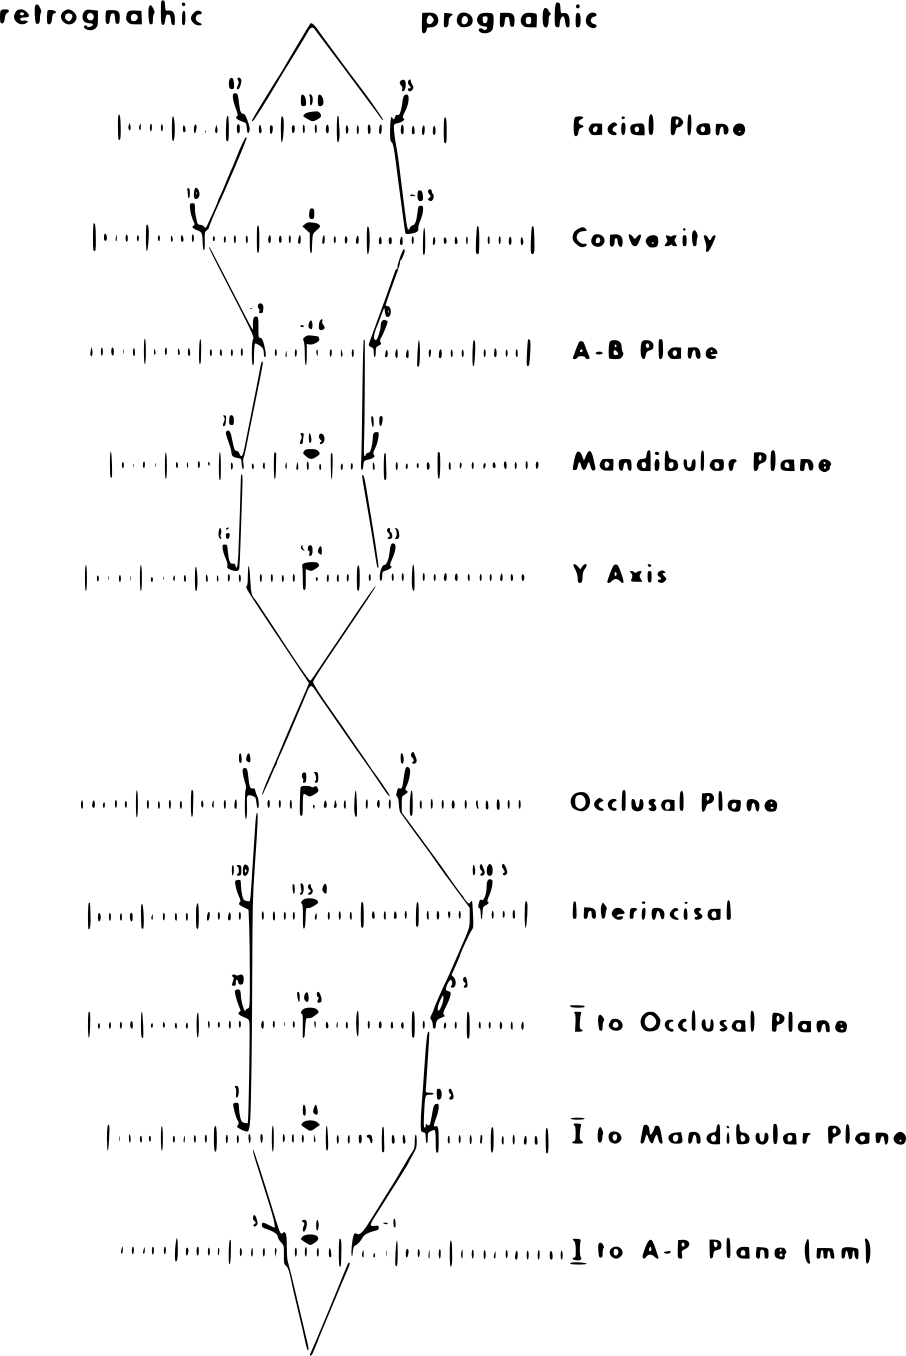
\includegraphics[width=.45\textwidth]{./images/downs.pdf}}
% downs.jpg: 1025x1440 pixel, 72dpi, 36.16x50.80 cm, bb=0 0 1025 1440
\caption{L'analisi di Downs enfatizza le variazioni individuali dal pattern facciale medio. Può servire come una guida all'interpretazione di analisi cefalometriche per realizzare piani di trattamento più conformi alla realtà.}
\label{fig:downs}
\end{figure}

La prima analisi cefalometrica sviluppata negli Stati Uniti d'America fu quella di Downs, che mirava ad illustrare la \textit{diffusione} di tutte le misure di un individuo, disegnando questi valori su un grafico a $\pm1$ e $\pm2$ deviazioni standard da una linea verticale che rappresentava il punto centrale della distribuzione di ogni variabile (fig.~\vref{fig:downs}). Quest'analisi enfatizzò la consistenza delle differenze individuali attorno alla media statistica, e aiutò a sviluppare modelli di studio dello sviluppo individuale della faccia che erano spesso più realistici dei risultati cefalometrici.

Considerato che la correzione dei dismorfismi è basata sulla premessa che, con la normalizzazione della dentatura e della faccia, si migliori la funzionalità generale, la terapia è condizionata dalle caratteristiche individuali del pattern facciale del singolo paziente. In altre parole, è la \textbf{\textit{norma individuale}} a determinare il piano di trattamento, così come enfatizzato da Andresen nel 1931\footcite{Andresen1931,Andresen1944}.

Una volta riconosciuto il concetto di norma individuale, il processo diagnostico diventa un'equazione complessa. Diventa necessario identificare diverse incognite per determinare le indicazioni, e le controindicazioni, di un trattamento, e gli obiettivi dello stesso in termini di necessità e benefici. L'ortodonzista deve quindi valutare:

\begin{itemize}
\item l'impatto psicosociale dei cambiamenti dentofacciali;
\item l'impatto psicologico della malocclusione sulla funzionalità labiale, i movimenti mandibolari, la respirazione, la crescita e lo sviluppo, la masticazione e la salute orale;
\item gli aspetti anatomici del disallineamento dentale, dell'occlusione e delle relazioni dentali, della forma, disarmonia o dell'asimmetria facciale, e della configurazione dei tessuti molli.
\end{itemize}

In breve, la diagnosi deve basarsi sulla valutazione del paziente \textit{in toto}, non escludendo alcun ambito. La pianificazione del trattamento deve basarsi sul conseguimento di un \textit{optimum} estetico e funzionale per ogni singolo paziente, piuttosto che l'aderenza a norme codificate. L'occlusione ideale, e la divina proporzione, possono quindi essere, al più, degli indicatori della giusta direzione da intraprendere.

\section{Scopo della tesi, materiali e metodi}
Questo studio si propone quindi di presentare alcune tecniche di analisi cefalometrica, di seguito definite \textit{proporzionali}, e di valutarne il differente impatto in termini diagnostici rispetto a quelle tecniche che si basano su \textit{valori ideali} comuni per tutti, statisticamente rilevati.

In particolare, verranno prese in esame, a livello teorico, le seguenti tecniche:
\begin{itemize}
\item analisi statistiche
\begin{itemize}
\item Downs
\item Steiner (secondo Giannì)
\item Ricketts
\end{itemize}
\item analisi proporzionali
\begin{itemize}
\item analisi delle controparti di Enlow
\item analisi proporzionale di Coben
\item analisi architetturale di Delaire
\item la rosa dei venti di Sassouni
\end{itemize}
\end{itemize}

\subsection{Disegno sperimentale}
Verranno prese in esame 29 teleradiografie in proiezione latero-laterale con craniostato, e di ognuna verrà effettuata un'analisi di tipo statistico (Giannì), e due di tipo proporzionale (Enlow, Coben). Queste verranno quindi comparate in termini diagnostici secondo diversi parametri. Tra questi verrà considerata la classe scheletrica, per la quale saranno presi in considerazione anche l'indice Wits\footcite{Jacobson1975} e gli appropriati valori dell'analisi di Ricketts. Scopo della tesi è quindi di valutare l'eventuale concordanza o discordanza tra le diverse analisi cefalometriche considerate.

\chapter{Cenni di storia della cefalometria}
Storicamente, la forma umana è stata misurata per diversi motivi: la scultura, il disegno o la pittura; oppure la relazione tra la forma e la salute, il temperamento, o i tratti comportamentali.

Gli ortodontisti e i chirurghi plastici e maxillo-facciali hanno contribuito a questi sforzi con i loro studi sul volto e il profilo umano, alla ricerca di linee guida per la ricostruzione di dismorfismi facciali e la correzione di malocclusioni. I principi base per questi studi sono stati enunciati fin dall'antichità.

Le radici della cefalometria affondano quindi nell'arte antica, grazie agli studi effettuati da artisti-scienziati che andavano alla ricerca della forma perfetta.

\section{Misure e proporzioni}
Ritrarre la forma umana richiede non solo talento artistico e capacità tecniche, ma anche uno stile consistente e disciplinato. Per assicurare queste premesse, gli antichi Egizi svilupparono un sistema quantitativo che definì le proporzioni del corpo umano, da usare quando venivano commissionate immagini regali e divine. Questo sistema divenne noto come \textit{canone}\footcite{Schaefer1963,Mueller1973,Iversen1975}.

La teoria delle proporzioni, secondo Panofsky\footcite{Panofsky1974}, è un:
\begin{quotation}
\textit{sistema per stabilire le relazioni matematiche tra le varie componenti di una creatura vivente, in particolare degli esseri umani, cosicché questi possano diventare soggetti di rappresentazione artistica. Tali relazioni matematiche possono essere espresse dalla divisione di un intero, così come dalla moltiplicazione di un'unità; lo sforzo di determinarle può essere guidato dal desiderio della bellezza, o dall'interesse nella normalità, o infine dalla necessità di stabilire una convenzione.}
\end{quotation}

Il canone veniva disegnato con la testa, i piedi e le gambe di profilo, e il torace in visione frontale. L'unità di misura per determinare l'altezza della figura, così come livelli anatomici intermedi come il ginocchio, il tronco e la spalla, era la lunghezza del piede. I piedi erano separati tra loro di una lunghezza pari a $\frac{2}{5}$ di piede. Venivano quindi disegnate linee orizzontali perpendicolari ad una linea verticale che divideva il corpo a metà. Il canone veniva quindi racchiuso in un sistema a griglia di quadrati con 18 linee orizzontali e 18 linee verticali. Nel tardo canone dell'arte Egizia, il corpo umano veniva racchiuso in una griglia di 22 linee orizzontali, con la linea 21 disegnata passante per la palpebra superiore.

\begin{figure}[h!]
\centering
\includegraphics[width=.35\textwidth]{./images/egizi_canone_piede.pdf}
% egizi_canone_piede.pdf: 421x708 pixel, 72dpi, 14.85x24.98 cm, bb=0 0 421 708
\caption{Uno dei primi canoni egizi.}
\label{fig:egyptian_canon}
\end{figure}

Diverse illustrazioni di arte Egizia mostrano anche come i tre riquadri superiori del canone venissero divisi a loro volta in cinque parti ognuno, per poter disegnare il volto con più dettagli.

Le arti classiche dei Greci rifiutarono il rigido sistema Egizio per creare immagini della figura umana, che non era adatto a rappresentarne i movimenti. I Greci concepivano infatti l'arte come rappresentazione di un essere vivo, in contrasto agli Egizi, che cercavano di cristallizzare la figura umana per l'eternità.

Nell'iconometria Indiana, l'altezza facciale era utilizzata come modulo base dai due sistemi proporzionali, Śāriputra e Ālekhyalakṣaṇa, che riflettevano accuratamente le relazioni naturali delle diverse parti del corpo tra di loro. Il sistema Śāriputra, datato 1200 d.C., è conosciuto per le sculture in onore di Buddha (fig. \vref{fig:sariputra_buddha}).

\begin{SCfigure}[][h!]
\centering
\subfloat[][]
   {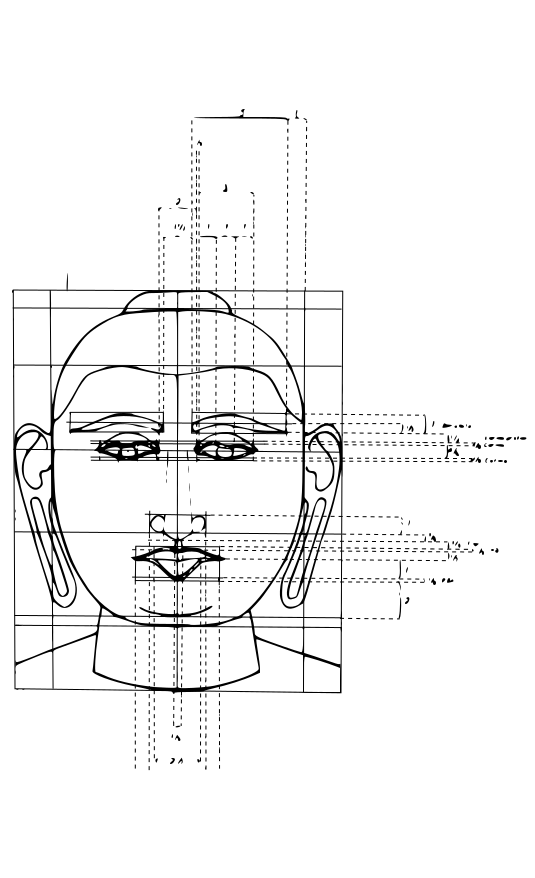
\includegraphics[width=.35\textwidth]{./images/sariputra_buddha_front.pdf}} \quad
\subfloat[][]
   {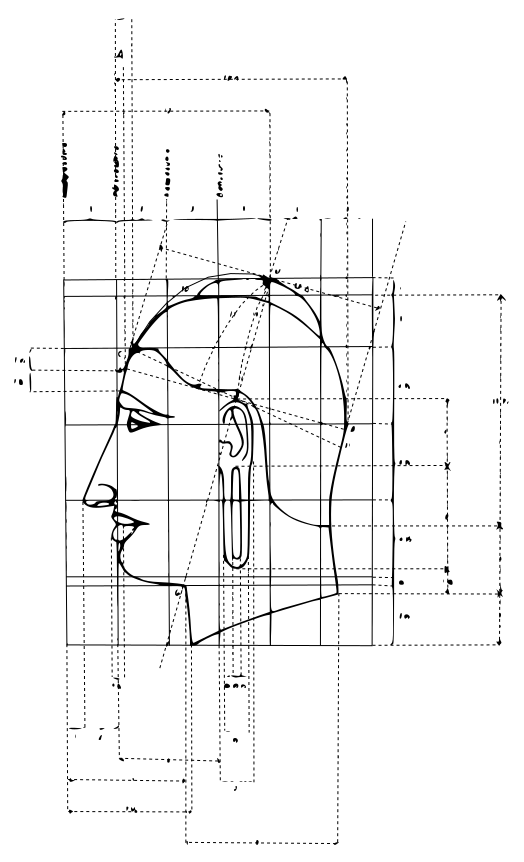
\includegraphics[width=.35\textwidth]{./images/sariputra_buddha_side.pdf}}
\caption{Visione frontale (a) e laterale (b) di una statua del Buddha, secondo il sistema proporzionale Śāriputra.}
\label{fig:sariputra_buddha}
\end{SCfigure}

\begin{wrapfigure}{L}{.4\textwidth}
 \centering
 
\includegraphics[width=.4\textwidth]{./images/byzantin_canon.pdf}
 \caption{Sistema a tre cerchi concentrici nell'arte Bizantina.}
 \label{fig:byzantin_canon}
\end{wrapfigure}

Nell'impero Bizantino, la griglia rettangolare del canone venne sostituita da uno schema di tre cerchi concentrici, con la lunghezza del naso come raggio per disegnare i due cerchi successivi. Il cerchio interno delineava la fronte e gli zigomi; il secondo cerchio, con un raggio pari a due volte il naso, definiva le misure esterne della testa, inclusi i capelli e il limite inferiore del volto. Il cerchio più esterno attraversava il giugulo e formava l'aureola.

\section{Dal Rinascimento al ventesimo secolo}
Lo sconvolgimento che il quindicesimo secolo portò nel pensiero artistico, nei concetti e nella tecnica è esemplificato dalle opere di Leonardo da Vinci (1459--1519) e Albrecht Dürer (1471--1528). Il lascito di Leonardo come esponente del Rinascimento va ben oltre l'Ultima Cena e la Monna Lisa. I suoi disegni includono infatti studi sulle proporzioni facciali, e la proiezione di un sistema di coordinate sul volto di un ``uomo cavallo''. Queste ultime figure mostrano una preferenza per le ``analisi proporzionali'', e si può notare che ogni personaggio posa in ``natural head position'' (XXX).

\begin{figure}[h!]
\centering
\subfloat[][]
   {\includegraphics[width=.4\textwidth]{./images/leonardo1.jpg}} \quad
\subfloat[][]
   {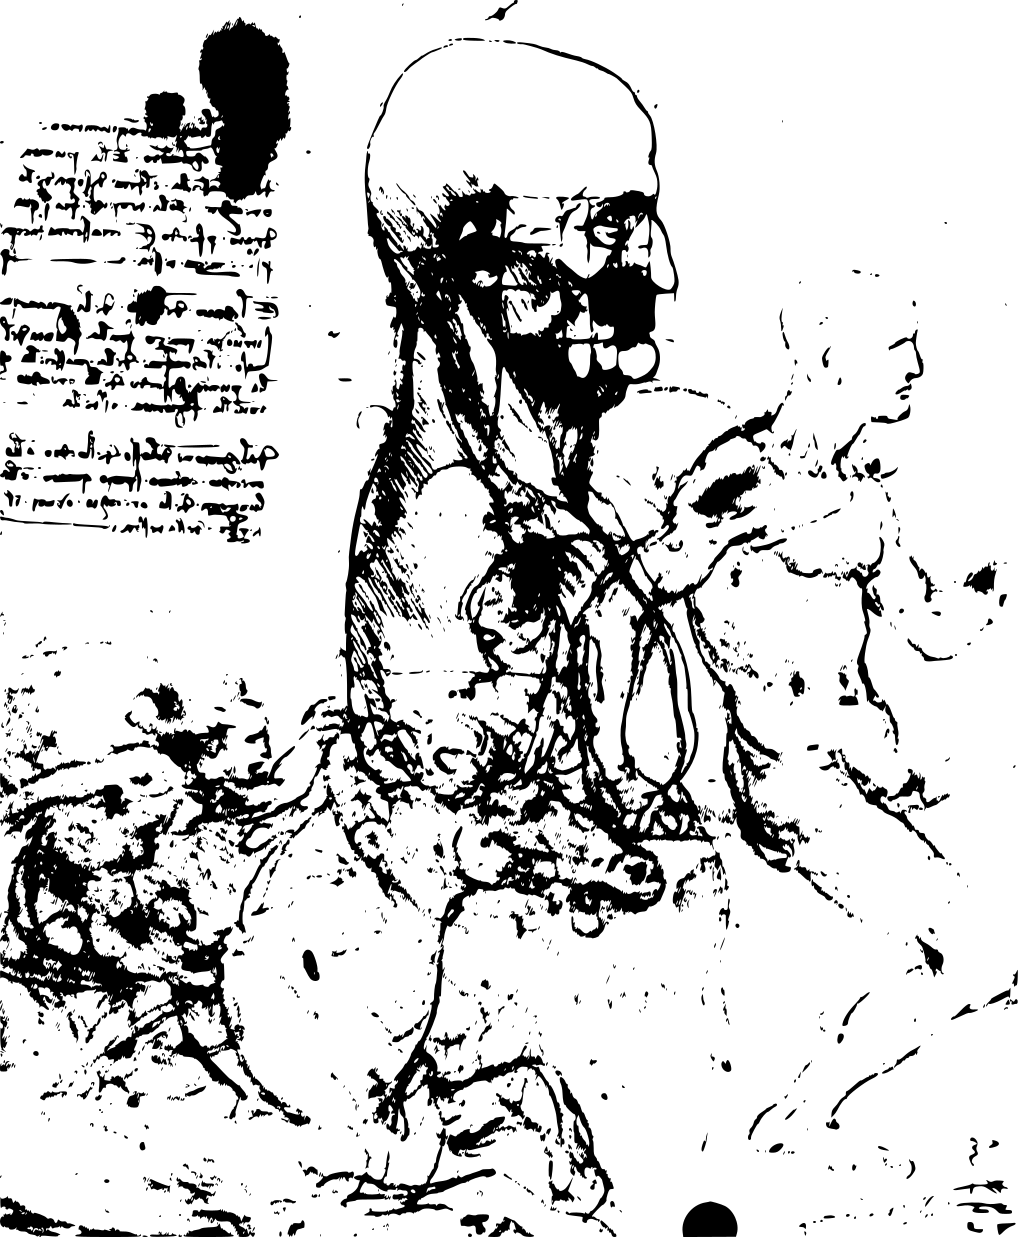
\includegraphics[width=.4\textwidth]{./images/leonardo2.jpg}}
\caption{Studi sul cranio e sul volto effettuati da Leonardo da Vinci.}
\label{fig:leonardo}
\end{figure}

Gli elaborati studi di Albrecht Dürer sulla prospettiva delle proporzioni umane sono ineguagliati ad oggi; infatti, i quattro libri di Dürer sulle proporzioni ``segnano un climax che la teoria delle proporzioni non ha mai raggiunto prima o avrebbe mai potuto raggiungere dopo''.\footcite{Panofsky1974}

\begin{SCfigure}[][h!]
\centering
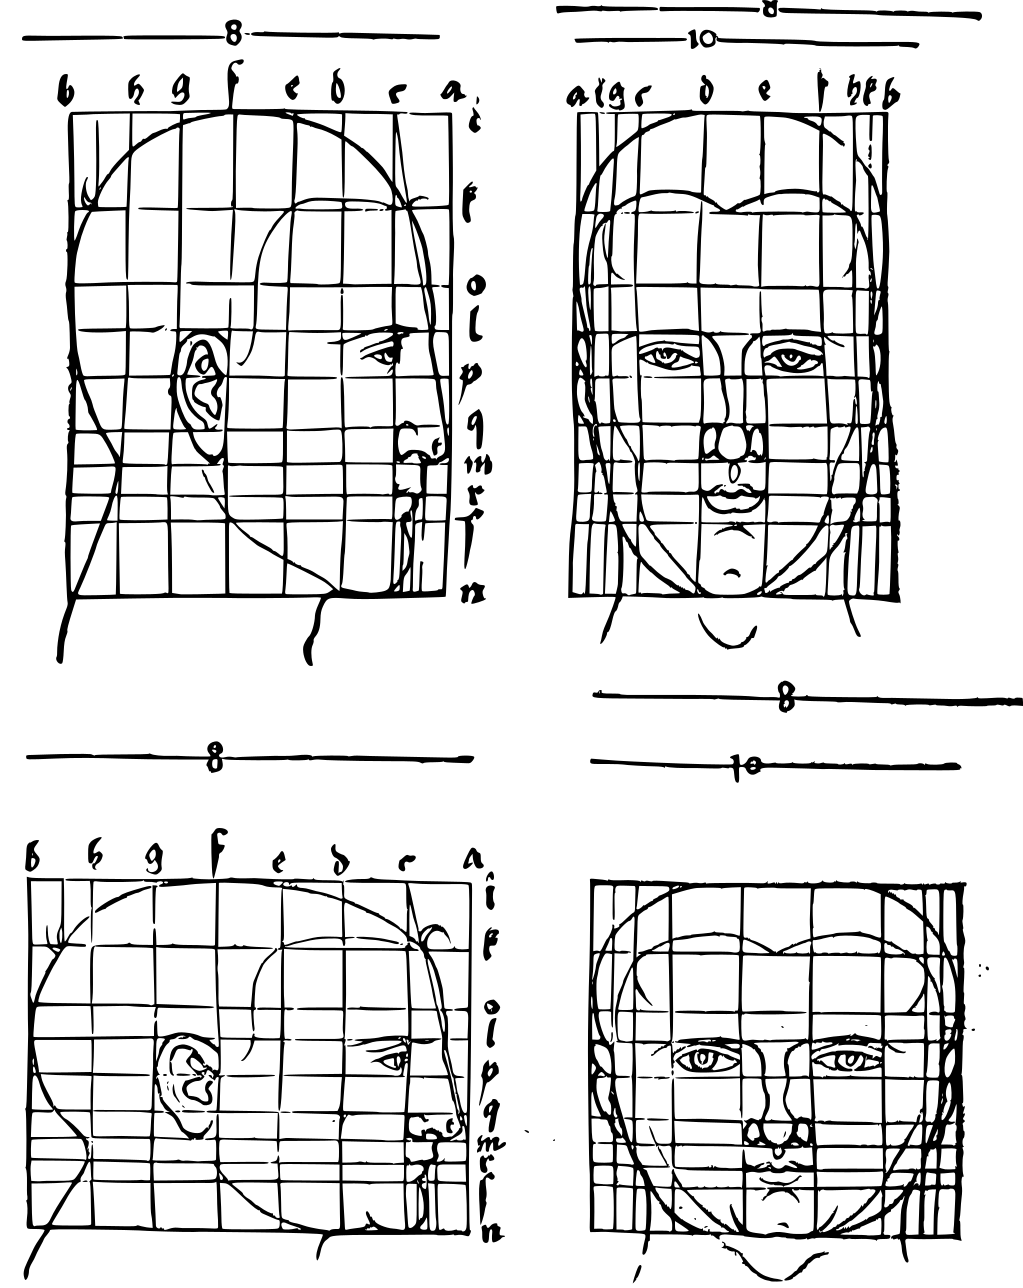
\includegraphics[width=.4\textwidth]{./images/duerer-proportional.jpg}
\caption{Analisi proporzionale di Dürer di un volto leptoprosopico ed uno euriprosopico.}
\label{fig:duerer}
\end{SCfigure}

Usando metodi strettamente geometrici, Dürer fornì un'analisi proporzionale dei volti leptoprosopici (stretti e lunghi) e dei volti euriprosopici (larghi e corti) in un sistema di coordinate in cui le linee orizzontali e verticali erano disegnate passanti per gli stessi punti facciali (fig. \vref{fig:duerer}).

\begin{wrapfigure}{R}{.4\textwidth}
\centering
\fbox{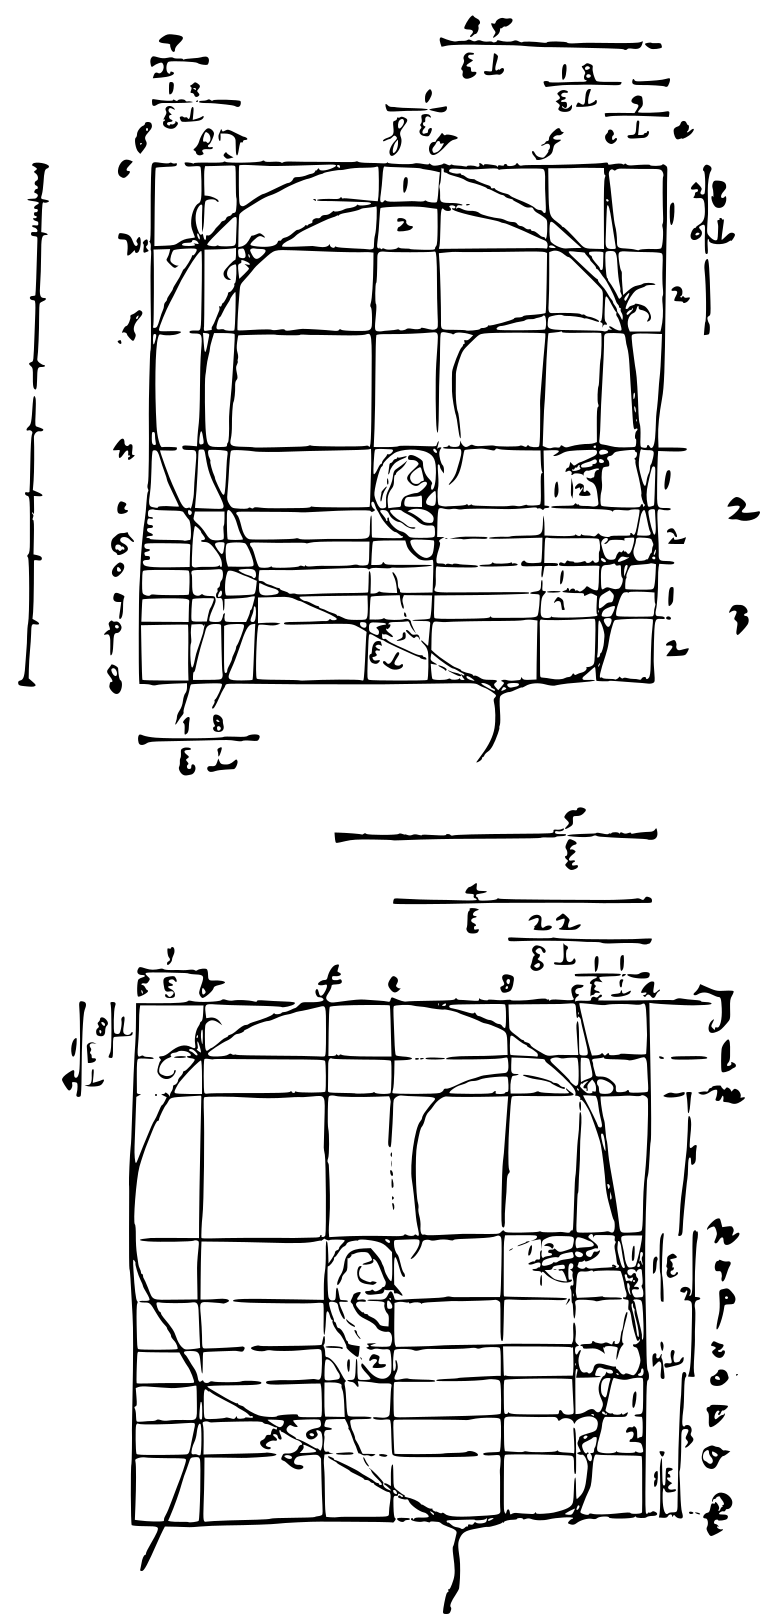
\includegraphics[width=.4\textwidth]{./images/duerer-proportional-2.jpg}}
\caption{Influenza dell'angolo facciale sul profilo secondo Dürer.}
\label{fig:duerer2}
\end{wrapfigure}

In aggiunta al sistema di coordinate, Dürer fece uso di due linee -- una disegnata dalla fronte tangente al naso, l'altra tangente al mento e al labbro superiore -- che insieme creavano un'area triangolare che caratterizzava il profilo facciale attraverso un ``angolo facciale'' (fig. \vref{fig:duerer2}).

I disegni di Dürer attestano i continui sforzi nel definire le variazioni della morfologia facciale. Uno di questi è particolarmente significativo, e rappresenta un punto chiave dell'evoluzione dell'analisi cefalometrica così come è conosciuta oggi. In esso, la differenza tra un profilo facciale retruso e uno protruso è mostrato da un cambiamento dell'angolo tra gli assi verticali e orizzontali di un sistema di coordinate caratterizzante la configurazione facciale di ogni soggetto. Perciò un singolo angolo diventa l'espressione della differenza nella morfologia facciale tra due individui.

%\begin{figure}[ht!]
% \centering
% 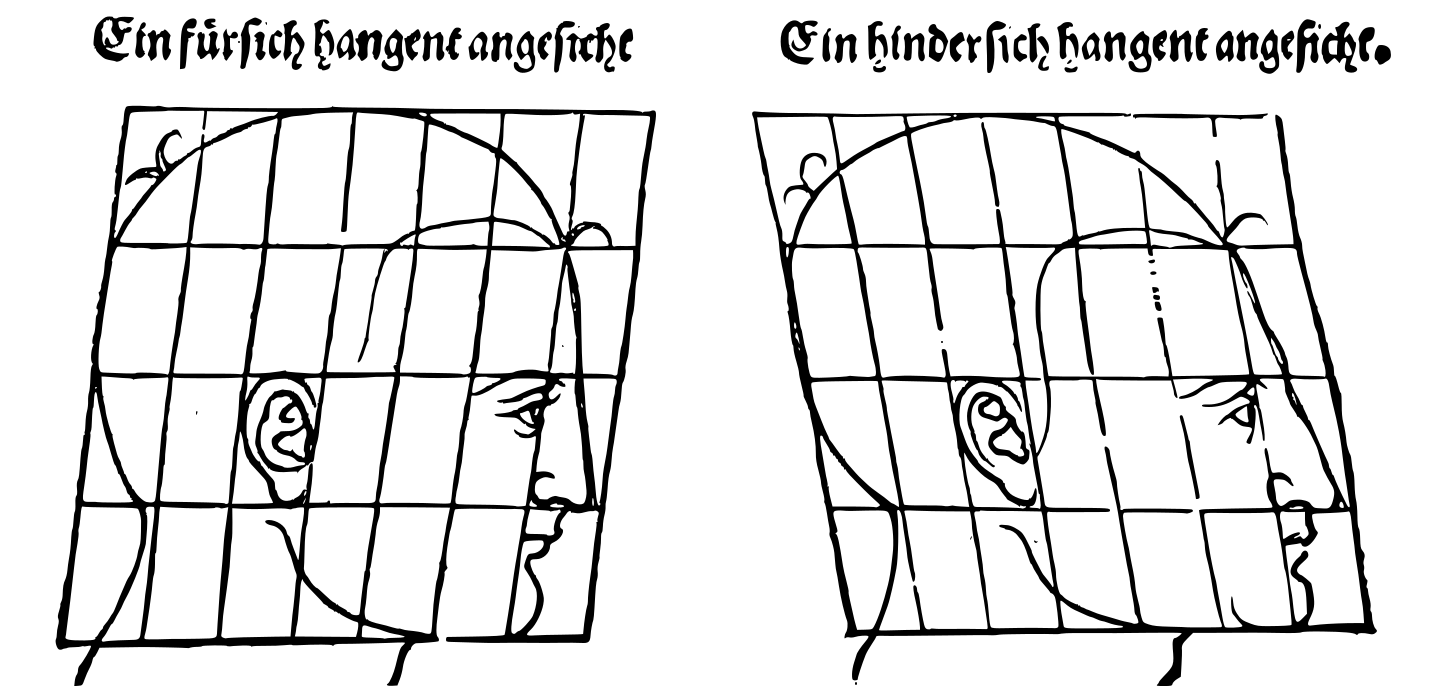
\includegraphics[width=.5\textwidth]{./images/duerer-proportional-3.jpg}
% % duerer-proportional-3.jpg: 1434x686 pixel, 72dpi, 50.59x24.20 cm, bb=0 0 1434 686
% \caption{sdf}
% \label{fig:duerer3}
%\end{figure}

Petrus Camper (1722--1789) fu un medico e scienziato che effettuò ampi studi sui crani. Il successo dei suoi studi si basava sull'orientamento dei crani nello spazio su un piano orizzontale, passante per il meato acustico esterno e un punto al di sotto del naso. Questi punti non erano rigorosamente definiti, ma Camper veniva guidato dalla direzione del processo zigomatico. In molte delle sue illustrazioni, questo piano orizzontale veniva disegnato passante per la spina nasale anteriore.

Il \textit{piano di Camper} divenne un piano di riferimento per le misure angolari utilizzate per caratterizzare gli andamenti evolutivi negli studi di morfologia facciale e sull'invecchiamento. Questo piano viene ancora oggi utilizzato in protesi per stimare l'angolazione del piano occlusale nei pazienti edentuli, poiché è generalmente parallelo.

Egli vide come un singolo angolo descrivesse il profilo caratteristico di una faccia. Questa cambia nella sua totalità, ma l'angolo facciale è l'indice di una deformazione generale.

L'angolo facciale di Camper venne prontamente accettato come una misura standard nello studio del cranio. I termini \textit{prognatico} e \textit{ortognatico} sono legati alle illustrazioni di Camper della forma facciale negli uomini e nei primati. Come risultato, l'angolo tra il piano orizzontale e la linea Nasion-Prosthion divenne il metodo antropologico d'elezione per determinare il tipo facciale. Il termine \textit{prognatismo} si riferisce alla prominenza della mandibola rispetto alla fronte; \textit{ortognatismo} si riferisce invece ad  un profilo facciale piatto.

\begin{SCfigure}[][h!]
 \centering
 \fbox{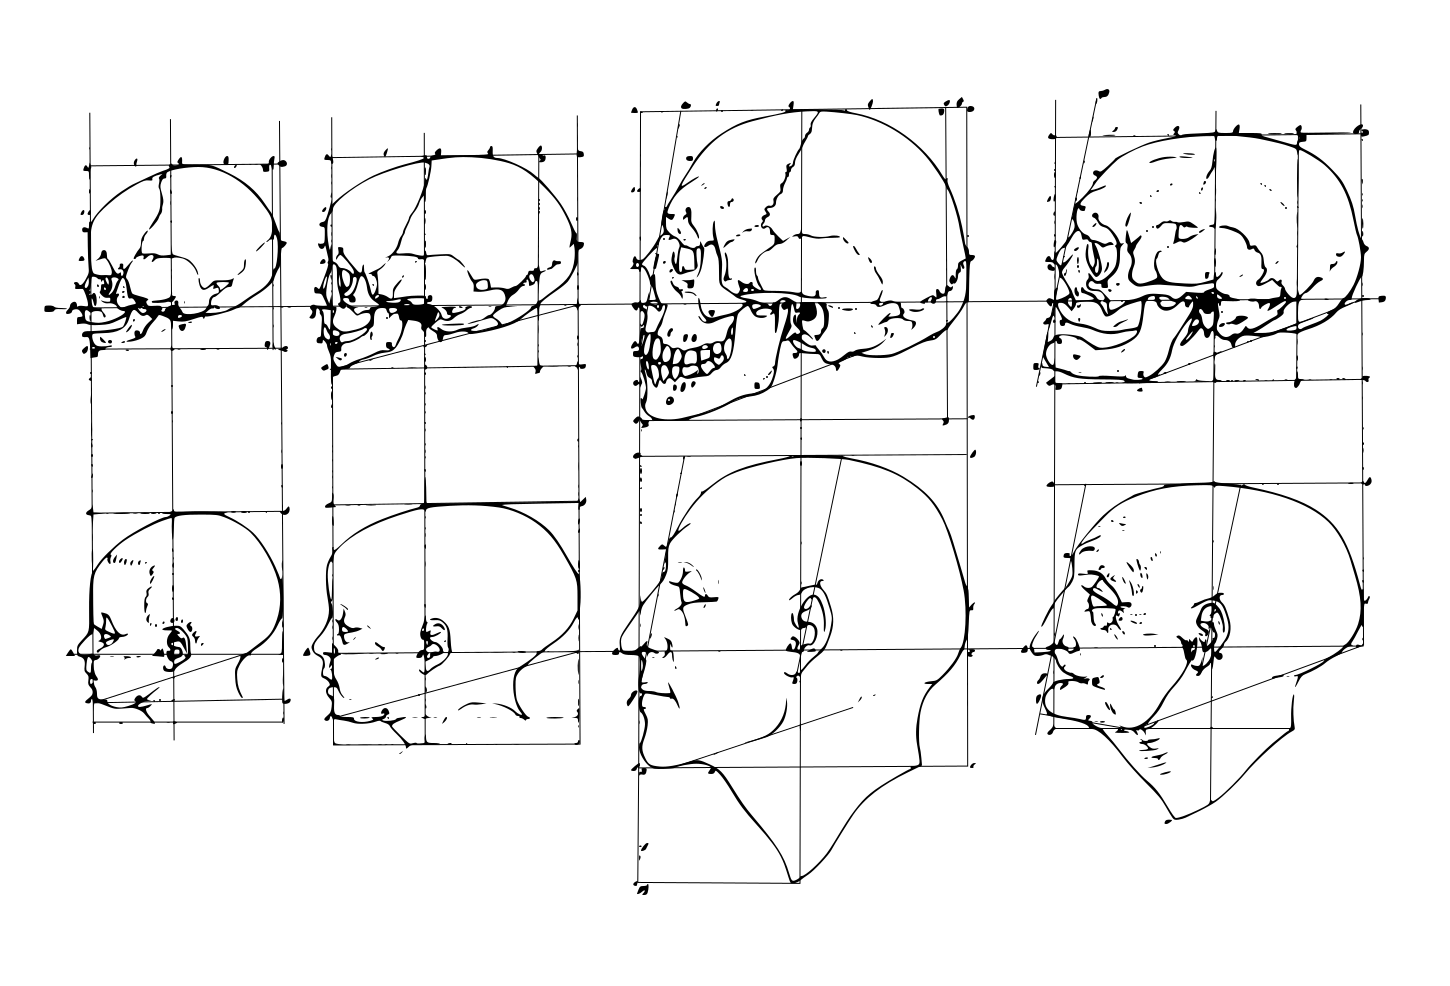
\includegraphics[width=.7\textwidth]{./images/camper-crani.pdf}}
 \caption{Studi di Camper sulle variazioni del cranio durante la crescita}
 \label{fig:camper-crescita}
\end{SCfigure}

Camper studiò anche le differenze nella forma facciale legate al processo di invecchiamento (fig. \vref{fig:camper-crescita}). La prima morfologia esaminata fu quella di un neonato, seguita da quella di un bambino di circa 8 anni, un adulto e un anziano. I cambiamenti vennero analizzati tenendo fisso il piano orizzontale, e consistono in una crescita della parte inferiore del volto fino all'età adulta, e il suo successivo accorciamento con la perdita progressiva di tutti i denti.

\begin{wrapfigure}{R}{.4\textwidth}
 \centering
 \fbox{\includegraphics[width=.4\textwidth]{./images/welcker-growth.pdf}}
 % welcker-growth.pdf: 695x709 pixel, 72dpi, 24.52x25.01 cm, bb=0 0 695 709
 \caption{Analisi dei cambiamenti durante la crescita secondo Welcker.}
 \label{fig:welcker}
\end{wrapfigure}

Gli studi di Welcker (1862) sulla crescita e lo sviluppo del cranio umano, dimostrarono la discesa e rotazione della mandibola durante l'ontogenesi, attraverso una configurazione triangolare dal Basion al Gnathion (fig. \vref{fig:welcker})\footcite{Welcker1866}. Questo schema triangolare fu successivamente modificato in un poligono da Hellman (fig. \vref{fig:hellman})\footcite{Hellman1935} per rappresentare la crescita facciale e per esaminare le differenze tra individui con malocclusioni di Classe II e Classe III. Dopo Hellman, questo poligono fu usato da Korkhaus\footcite{Korkhaus1939} e da Björk (fig. \vref{fig:bjork-profili})\footcite{Bjoerk1947}. Quest'ultimo sviluppò questo poligono in quella che può essere definita l'analisi ``forma-spazio'' dello scheletro facciale; analisi che illustrò chiaramente la configurazione facciale dalla base cranica al piano mandibolare, e dall'articolazione temporomandibolare al profilo facciale.

\begin{SCfigure}[][h!]
\centering
\fbox{\includegraphics[width=.7\textwidth]{./images/hellman-growth.pdf}}
% hellman-growth.pdf: 1070x605 pixel, 72dpi, 37.75x21.34 cm, bb=0 0 1070 605
\caption{Analisi della crescita facciale proposta da Hellman, usando un poligono e la linea da Nasion ad Auricolare come riferimento.}
\label{fig:hellman}
\end{SCfigure}

\begin{figure}[h!]
\centering
\subfloat[][]
   {\fbox{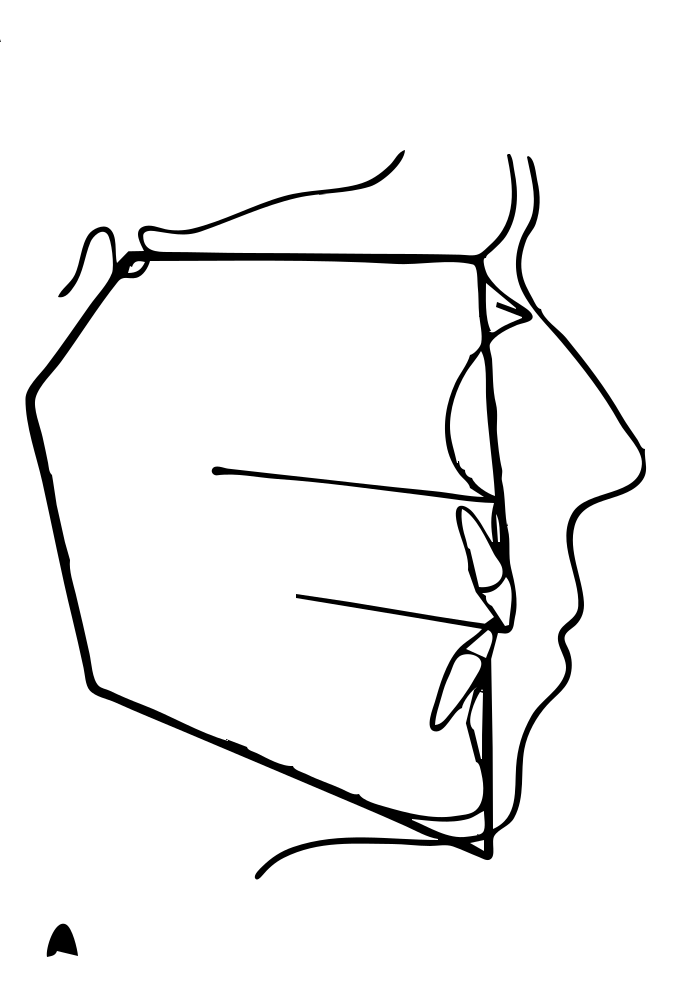
\includegraphics[width=.3\textwidth]{./images/bjork-a.pdf}}} \quad
\subfloat[][]
   {\fbox{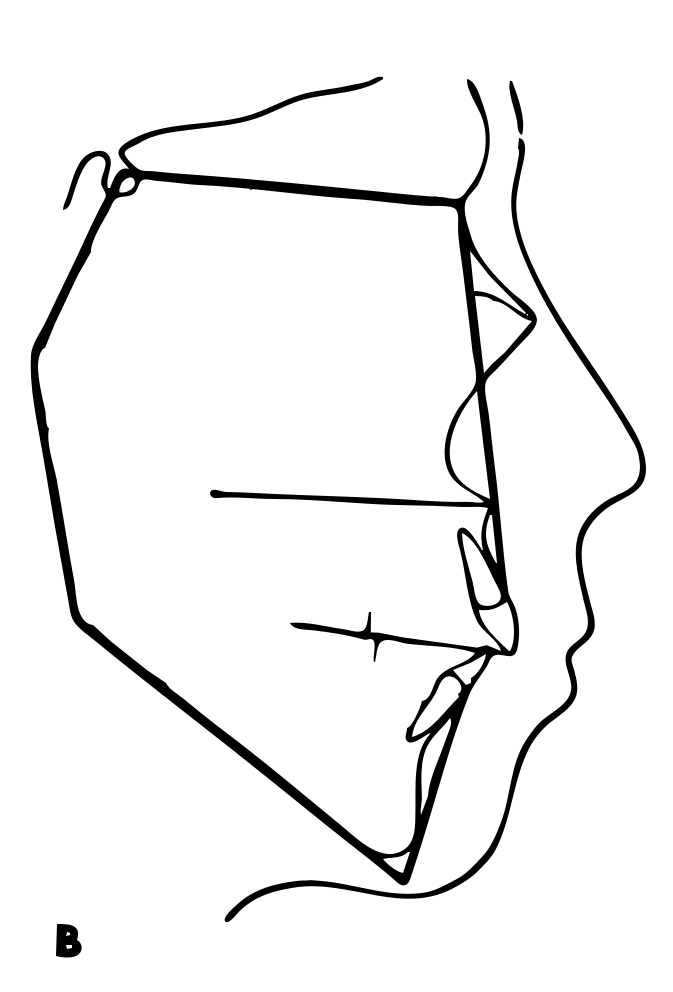
\includegraphics[width=.3\textwidth]{./images/bjork-b.pdf}}} \quad
\subfloat[][]
   {\fbox{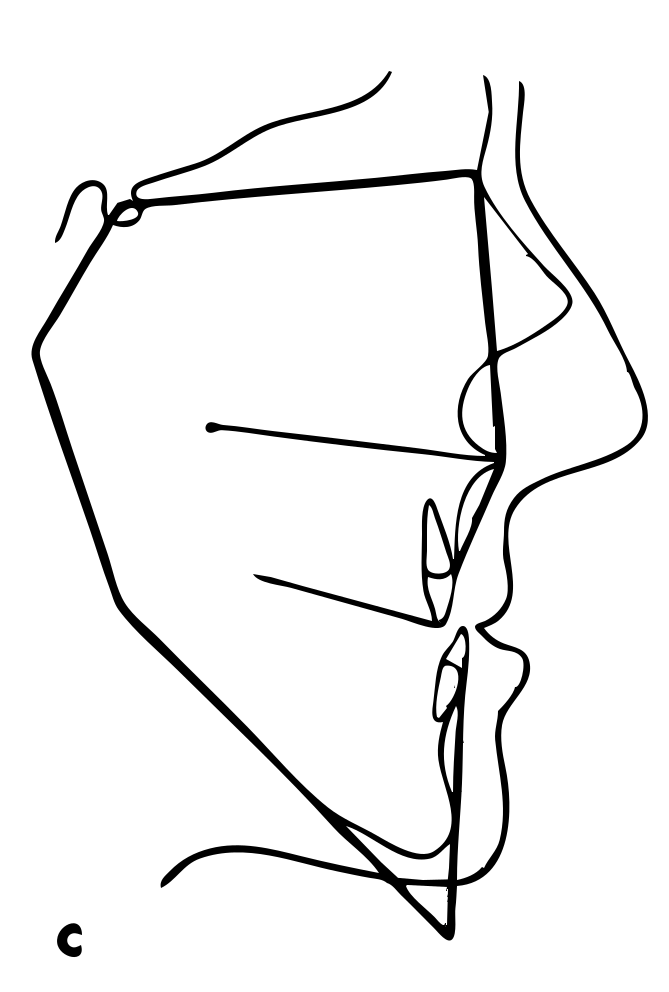
\includegraphics[width=.3\textwidth]{./images/bjork-c.pdf}}}
\caption{Studi di Björk sui profili facciali.}
\label{fig:bjork-profili}
\end{figure}

\subsection{Il ventesimo secolo}
L'evoluzione della cefalometria nel ventesimo secolo è universalmente collegata alla pubblicazione di Edward Angle sulle malocclusioni\footcite{Angle1899}, nel 1899. Angle usava le relazioni tra l'arcata superiore ed inferiore, esemplificata dall'intercuspidazione dei primi molari permanenti, come la base per caratterizzare i tipi di malocclusione.

\begin{SCfigure}[][t!]
\centering
\includegraphics[width=.7\textwidth]{./images/vanloon.jpg}
% vanloon.jpg: 1436x860 pixel, 72dpi, 50.66x30.34 cm, bb=0 0 1436 860
\caption{van Loon costruì un modello tridimensionale del profilo facciale, per poter meglio studiare i rapporti tra quest'ultimo e la dentatura del paziente.}
\label{fig:vanloon}
\end{SCfigure}

Un avanzamento concettuale in senso realistico fu fatto nel 1915 da van Loon, che determinò che per una diagnosi e un piano di trattamento significativi era necessario un sistema tridimensionale che potesse determinare la relazione della dentatura con la faccia. Egli sviluppò quindi un metodo con cui la dentatura e la faccia potessero essere studiati sia separatamente, sia in relazione l'uno con l'altro. Il metodo consisteva nel prendere un'impronta parziale del profilo (fronte, naso, labbra, mento), e delle superfici labiali degli incisivi centrali superiori -- quest'ultimi sarebbero serviti come chiave per il posizionamento del modello delle arcate dentarie. Questa ``maschera facciale'' (fig. \vref{fig:vanloon}) veniva poi posizionata su un supporto all'interno di un ``cubo cranioforo''. Questo era uno strumento utilizzato dagli antropologi per studiare i crani orientati secondo il piano di Francoforte. Sebbene questa procedura fosse complessa, lunga e poco pratica, è da segnalare in quanto rappresenta un passo evolutivo verso il posizionamento dei modelli dentari orientati tridimensionalmente nello spazio.

\begin{wrapfigure}{R}{.5\textwidth}
\centering
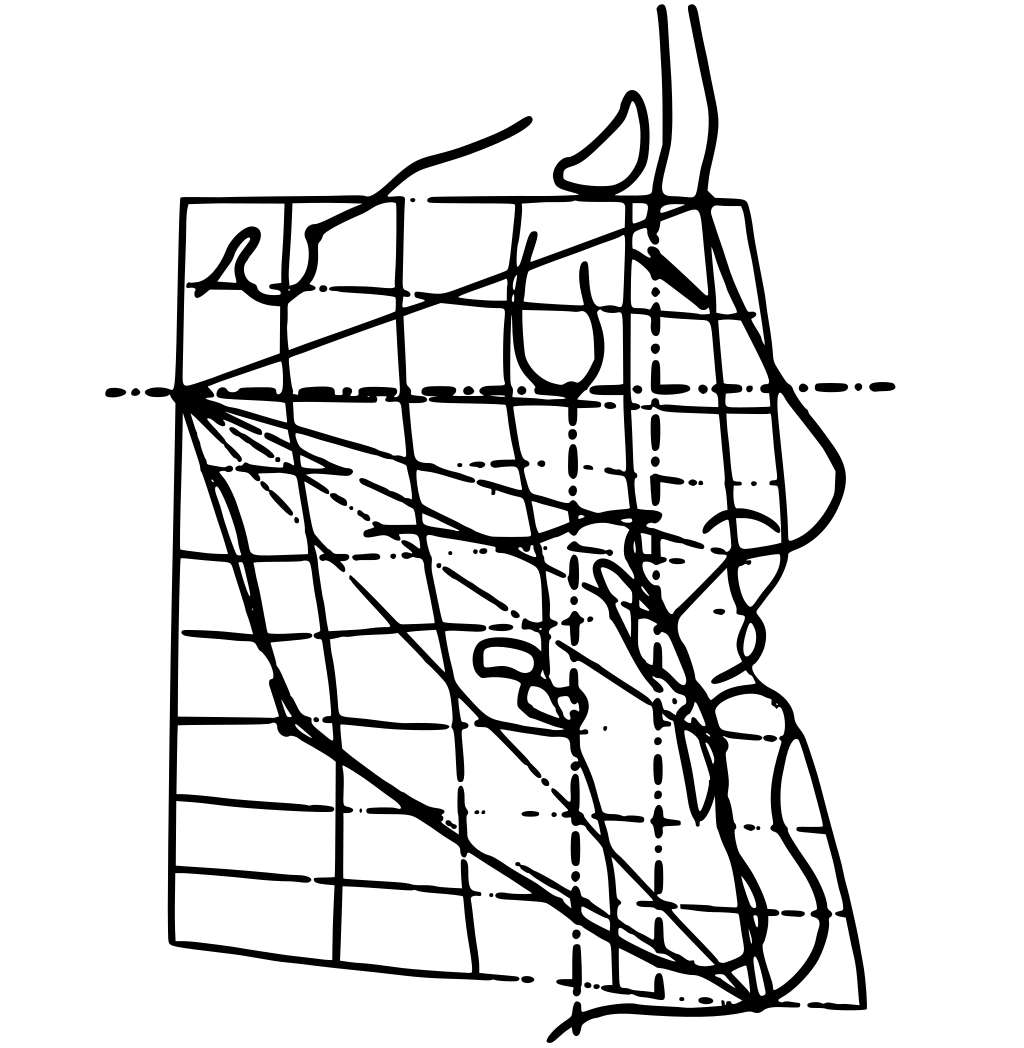
\includegraphics[width=.5\textwidth]{./images/decoster.pdf}
% decoster.pdf: 819x838 pixel, 72dpi, 28.89x29.56 cm, bb=0 0 819 838
\caption{De Coster: analisi di un individuo con marcato prognatismo mandibolare e severa malocclusione di Classe III.}
\label{fig:decoster}
\end{wrapfigure}

In seguito alla standardizzazione della radiografia cefalometrica agli inizi del 1900, Lucien de Coster\footcite{Coster1939} fu il primo a pubblicare un'analisi basata sulle relazioni di proporzionalità usate nell'antichità (fig. \vref{fig:decoster}). De Coster utilizzò le distorsioni di un sistema di coordinate Cartesiano per mostrare le differenze di posizione dei marker in confronto alla norma\footcite{Izard1943}.

\section{La divina proporzione}

Fin dai primi dati disponibili, i ritratti del corpo umano sono stati guidati da sistemi di proporzionalità tra le sue parti. Questa procedura consentiva la riproduzione di relazioni armoniose tra le caratteristiche facciali e il resto del corpo.

\begin{wrapfigure}{R}{.5\textwidth}
\centering
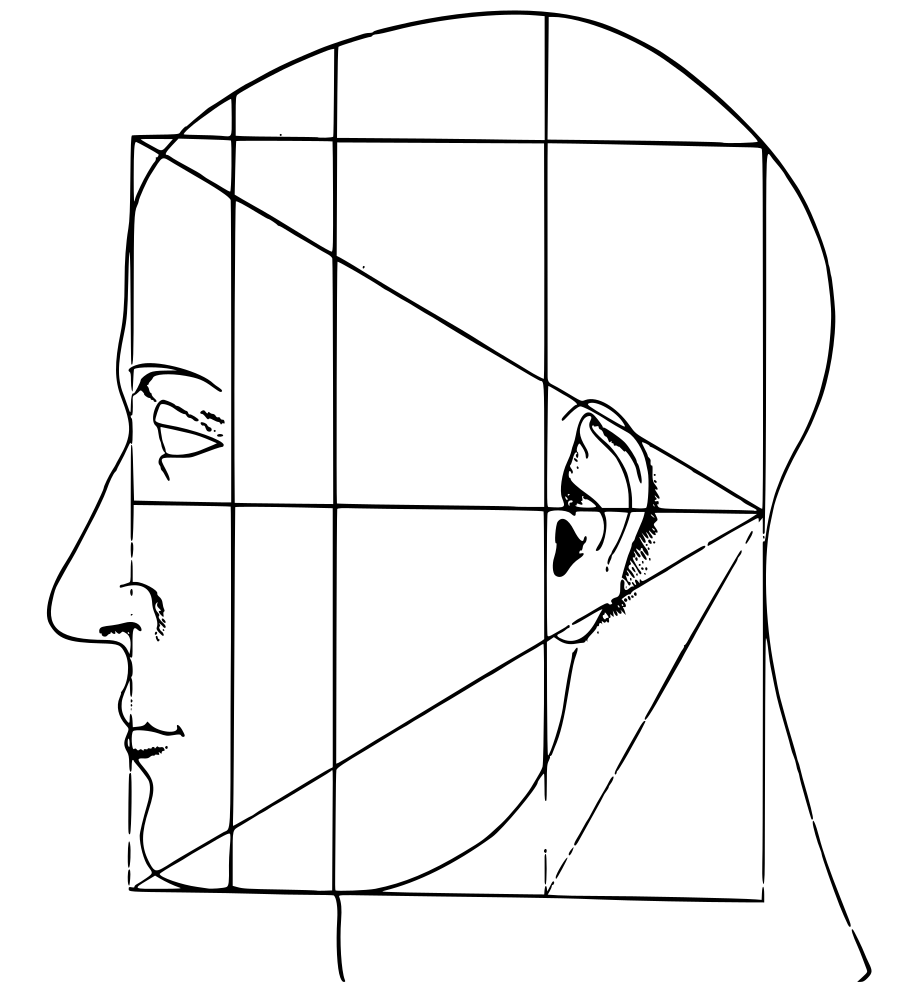
\includegraphics[width=.5\textwidth]{./images/pacioli.pdf}
% pacioli.pdf: 733x794 pixel, 72dpi, 25.86x28.01 cm, bb=0 0 733 794
\caption{Nel 1509, fra' Luca Pacioli, nella sua presentazione sulla divina proporzione, mostrò un'illustrazione di un profilo umano inquadrato in un triangolo ed un rettangolo aureo.}
\label{fig:pacioli}
\end{wrapfigure}

Nella \textit{sezione aurea} (la ``\textit{divina proporzione}''), sviluppata dagli antichi matematici Greci, la lunghezza di una linea è divisa in due parti tali che la parte minore, divisa per la parte maggiore, è uguale alla parte maggiore divisa per la lunghezza totale. Oltre ad avere applicazioni matematiche, la sezione aurea costituisce un ideale per le valutazioni di natura estetica.

Nel 1509, Luca Pacioli\footcite{Pacioli1509}, presentò un'orazione sulla sezione aurea in ambito matematico. La sua pubblicazione conteneva un disegno di un profilo umano, inquadrato in un triangolo ed un rettangolo aureo (fig. \vref{fig:pacioli}).

Nella progettazione del volto umano, la Natura ha evidentemente trasposto la \textit{divina proporzione} in una sequenza di relazioni armoniose tra i tessuti molli e i tessuti duri. %Paradies\footnote{biblio 40} ha dimostrato che la sezione aurea è la chiave per determinare l'altezza facciale inferiore nella riabilitazione di pazienti edentuli.

Ricketts\footcite{Ricketts1982,Ricketts1982a} fu il primo, nella storia recente, ad esporre in dettaglio sulla relazione tra la struttura e la crescita della faccia e la divina proporzione e la serie di Fibonacci.

\chapter{Crescita cranio-facciale}
\nocite{Enlow1986,Cozza2006}

Le teorie di crescita rappresentano le ipotesi postulate nel corso dell'evoluzione scientifica al fine di spiegare e identificare i fattori responsabili dello sviluppo del complesso cranio-facciale.

Per meglio utilizzare le tecniche di analisi cefalometrica più avanti descritte, l'or\-to\-don\-ti\-sta deve conoscere i comuni meccanismi di crescita, per sapere in quale momento è necessario intervenire, e capire le condizioni che possono favorire la stabilità del risultato terapeutico o, al contrario, causarne la recidiva.

L'analisi dell'evoluzione storica sull'argomento ha permesso di dividere le teorie di crescita in tre gruppi principali:
\begin{enumerate}
\item corrente di pensiero genetica (1931-1946)
\item corrente di pensiero funzionalistica (1945-1990)
\item corrente di pensiero sintetica o del consenso (1970)
\end{enumerate}

\section{Corrente di pensiero genetica (1931-1946)}
Le prime teorie sul processo di crescita ritenevano che il meccanismo principale era sotto un costante e rigoroso controllo genico. Tale condizione metteva fortemente in discussione l'efficacia dell'ortopedia dento-facciale in generale, e di quella funzionale in particolare.

La crescita del cranio è predeterminata, e non è soggetta ad alcuna influenza esterna, pertanto anche le dismorfosi dento-maxillo-facciali sono manifestazioni di caratteri ereditari.

\subsection*{Teoria della predeterminazione genetica\protect\footcite{Broadbent1931,Broadbent1937,Brodie1941,Brodie1946}}
La prima teoria postulata nel corso della letteratura affermava che le disgnazie esistono prima della nascita, codificate nei geni, e che durante la crescita post-natale non migliorano e non peggiorano, pertanto quando un neonato nasce con una disgnazia, questa permane tutta la vita, e non può essere trattata in alcun modo.

\subsection*{Ipotesi suturale\protect\footcite{Weinmann1956}}
Le suture, la cartilagine e il periostio sono ``centri autonomi'' di crescita sotto il controllo genico, e non influenzabili da fattori locali né dalla terapia. Ci si sposta quindi da una teoria in cui tutto è sotto il controllo genico, ad una in cui l'attività genica si limita a quei tessuti capaci di generare osso.

\subsection*{Ipotesi del setto nasale\protect\footcite{Scott1967}}
Tale ipotesi si basa sul ruolo svolto dalle strutture cartilaginee del cranio durante lo sviluppo fetale, e sulla possibilità che esse continuino il loro ruolo di guida dello sviluppo anche post-nascita.

Il controllo genico si sposta quindi sulle strutture cartilaginee, che diventano le uniche responsabili del processo di crescita cranio-facciale.

In particolare, la cartilagine del setto nasale è responsabile della crescita del mascellare superiore: con il suo sviluppo, si ha una spinta verso il basso e in avanti della premaxilla e, insieme alla \textit{cartilagine di Meckel}, partecipa in modo preponderante alla formazione della faccia.

La limitazione dell'influenza genica alle sole cartilagini apre quindi la strada ad una possibile influenza esterna sulle suture, sfruttabile in ambito terapeutico.

\section{Corrente di pensiero funzionalistica (1945-1990)}
La corrente funzionalistica mette in evidenza l'importanza della funzione nella realizzazione della crescita cranio-facciale, spostando l'attenzione dal pensiero genetico a quello funzionale.

L'influenza genetica è comunque presente in tutto lo sviluppo biologico; i tessuti hanno però un loro grado di plasticità e quindi sono influenzabili da fattori estrinseci al genoma.

Se la funzione rappresenta il fattore più importante per la crescita, sarà anche quello che alterandosi causerà una disgnazia; pertanto la riabilitazione della corretta funzione determina il recupero dell'equilibrio.

\subsection*{Ipotesi della matrice funzionale\protect\footcite{Moss1960,Moss1969}}
In questa teoria, è la funzione ad avere un'influenza diretta su forma, dimensione e posizione dei tessuti scheletrici; anche se esiste un controllo genico durante la fase iniziale della ossificazione, questo continua poi a livello funzionale. Le strutture ossee e cartilaginee non sono infatti dotate di un proprio schema di crescita, ma si accrescono secondariamente ai tessuti che li circondano (\textit{matrici funzionali}).

Secondo Moss, esistono delle funzioni vitali (tra cui masticazione, fonazione, deglutizione), ed ognuna di queste è svolta grazie a tessuti, organi, spazi e strutture scheletriche e cartilaginee. L'insieme delle entità anatomiche necessarie per eseguire una specifica funzione viene detta \textit{componente cranica funzionale}: ciascuna di queste è costituita da due elementi -- la \textit{matrice funzionale}, che svolge la funzione propria; e l'\textit{unità scheletrica} che svolge la funzione di protezione e di sostegno.

La grandezza, la forma e la posizione di ogni unità scheletrica rappresentano una risposta compensatoria alle richieste della matrice funzionale; l'unità scheletrica non è quindi direttamente regolata dal genoma, ma viene modulata dalla matrice funzionale.

Moss distingue due matrici funzionali:

\begin{enumerate}
\item la \textit{matrice funzionale periostale}, tipicamente associata a muscoli, vasi sanguigni, nervi e ghiandole;
\item la \textit{matrice funzionale capsulare}, costituita da capsule o involucri di tessuti non scheletrici che includono la loro unità scheletrica.
\end{enumerate}

La crescita a livello della matrice funzionale \textit{periostale} è di tipo \textit{trasformativo}, e si realizza attraverso processi di apposizione e riassorbimento osseo, che inducono una modificazione della forma e della dimensione della propria unità scheletrica. Le matrici di questo tipo hanno quindi influenza su \textit{microunità scheletriche} che, prese insieme, formano un intero osso.

Un esempio è la mandibola, che risulta costituita da 5 microunità: condilare, coronoidea, angolare, alveolare e basale. Il muscolo temporale è la matrice dell'unità coronoidea; il massetere e pterigoideo interno di quella angolare; i denti sull'unità alveolare, mentre il fascio vascolonervoso del canale mandibolare agisce sull'unità basale.

Per quanto riguarda le matrici funzionali capsulari, nel distretto cranio-facciale si riconoscono:

\begin{enumerate}
\item \textit{matrice funzionale capsulare neurocranica}, che rappresenta il volume della massa cerebrale;
\item \textit{matrice funzionale capsulare orofacciale}, di nostra pertinenza, che rappresenta il volume degli spazi funzionanti delle cavità oro-naso-faringee, orbitali e uditive.
\end{enumerate}

La crescita a livello delle matrici \textit{capsulari} è di tipo \textit{traslativo}, avviene cioè attraverso un processo di riposizionamento della propria unità scheletrica. La sfera d'influenza è rappresentata dalle \textit{macrounità scheletriche}. Ciascuna matrice funzionale capsulare, e ciascuna capsula, contiene quindi le matrici funzionali periostali e le rispettive microunità scheletriche.

Lo sviluppo di tutte le unità scheletriche cranio-facciali è quindi una combinazione di due tipologie di crescita:

\begin{enumerate}
\item \textit{trasformativa}, dovuta ai cambiamenti in forma e dimensione delle microunità scheletriche, in risposta allo stimolo delle matrici funzionali periostali;
\item \textit{traslativa}, dovuta ad un ricollocamento nello spazio delle macrounità scheletriche, in risposta all'aumento volumetrico degli spazi funzionanti e della massa cerebrale.
\end{enumerate}

L'insieme della crescita trasformativa e della crescita traslativa permette il mantenimento dell'equilibrio tra matrici funzionali e unità scheletriche, tale da realizzare una \textit{crescita armonica}.

\subsection*{Teoria del servosistema o teoria cibernetica\protect\footcite{Petrovic1974,Petrovic1981}}

Allo scopo di comprendere i meccanismi dello sviluppo craniofacciale, Petrovic e coll. hanno sviluppato la \textit{teoria del servosistema}, utilizzando il vocabolario proprio della cibernetica.

La cibernetica è una scienza che ha come obiettivo la comprensione sistematica della realtà, facendo confluire insieme una serie di nozioni e problemi patrimonio comune di più discipline (biologia, ingegneria, psicologia, meccanica). Tale scienza opera attraverso un circuito, il \textit{servosistema}, caratterizzato da un insieme di \textit{segnali di controllo} e \textit{di comando}, che schematizza come la trasmissione di tali segnali porta al verificarsi di un fenomeno.

La crescita delle differenti regioni del cranio diventa quindi la risultante dell'interazione di un insieme di avvenimenti e di meccanismi di feedback, che permettono al sistema di autoregolarsi.

Petrovic ha quindi sintetizzato le sue idee nella teoria cibernetica dei processi di controllo della crescita cranio-facciale, attraverso la costruzione di un \textit{servosistema}.

In generale, all'interno di un servosistema esiste un \textit{comparatore periferico} che opera un confronto tra un \textit{input} (variabile indipendente) e un \textit{output} (variabile controllata), e invia un messaggio al \textit{comparatore centrale}, che regola i fattori di controllo di un determinato fenomeno per mantenere l'equilibrio. Nel servosistema ideato da Petrovic, il comparatore periferico è rappresentato dall'\textit{occlusione}, quello centrale è il \textit{sistema nervoso centrale}, l'input è il \textit{mascellare superiore}, e l'output è la \textit{mandibola}.

L'occlusione, quindi, opera un confronto tra la posizione del mascellare superiore e la posizione della mandibola, e invia un messaggio al sistema nervoso centrale, che regola i fattori di controllo della crescita per mantenere l'equilibrio.

Il mascellare superiore è considerato la variabile indipendente in quanto è controllato solamente da fattori estrinseci generali (ormoni), e non può in alcun modo essere influenzato da fattori locali. La mandibola, invece, oltre a subire il controllo ormonale, è anche sottoposta a fattori estrinseci locali (muscoli, legamenti).

\part*{Analisi convenzionali}
\chapter{Analisi di Downs}
\nocite{Enlow1986,Vorhies1951,Downs1956}

L'analisi di Downs si può definire un'analisi ``\textit{profilo-orientata}''. Il piano di riferimento è quello di Francoforte, e la valutazione verticale è fatta unicamente tramite il piano mandibolare e l'asse Y. Quest'analisi non presenta punti cefalometrici propri, ma si basa su misure utilizzate in numerose altre analisi.

{\Huge FIXME!}

Spesso quest'analisi viene accompagnata da una \textit{tabella di Voorhies e Adams}, che fornisce un quadro grafico delle dieci misurazioni dell'analisi.

In quest'analisi distinguiamo misurazioni ossee da misurazioni dentali (graficamente separate nel poligono di Voorhies e Adams).

\section{Misurazioni ossee}
\begin{table}[h]
%\footnotesize
\caption{Misurazioni ossee nell'analisi di Downs (valori in °)}
\begin{tabularx}{\textwidth}{>{\bfseries}lXcc}
\toprule
 & Punti di riferimento & Val. medio & Range normalità \\
\cmidrule(r){2-4}
Angolo facciale & \piano{Na}{Pog} -- \textit{FH} & 87.8 $\pm$ 3.6 & 82 -- 95 \\
Convessità facciale & \piano{Na}{A} -- \piano{A}{Pog} & 0 & -8.5 -- 10 \\
Piano \piano{A}{B} & \piano{A}{B} -- \piano{Na}{Pog} & -4.6 & -9 -- 0 \\
Piano mandibolare & \textit{MP} -- \textit{FH} & 21.9 & 17 -- 28 \\
Asse Y & \piano{S}{Gn} -- \textit{FH} & 59.4 & 53 -- 66 \\
\bottomrule
\end{tabularx}
\end{table}

\begin{figure}[h!]
\centering
\begin{minipage}{.44\textwidth}
 \centering
 \fbox{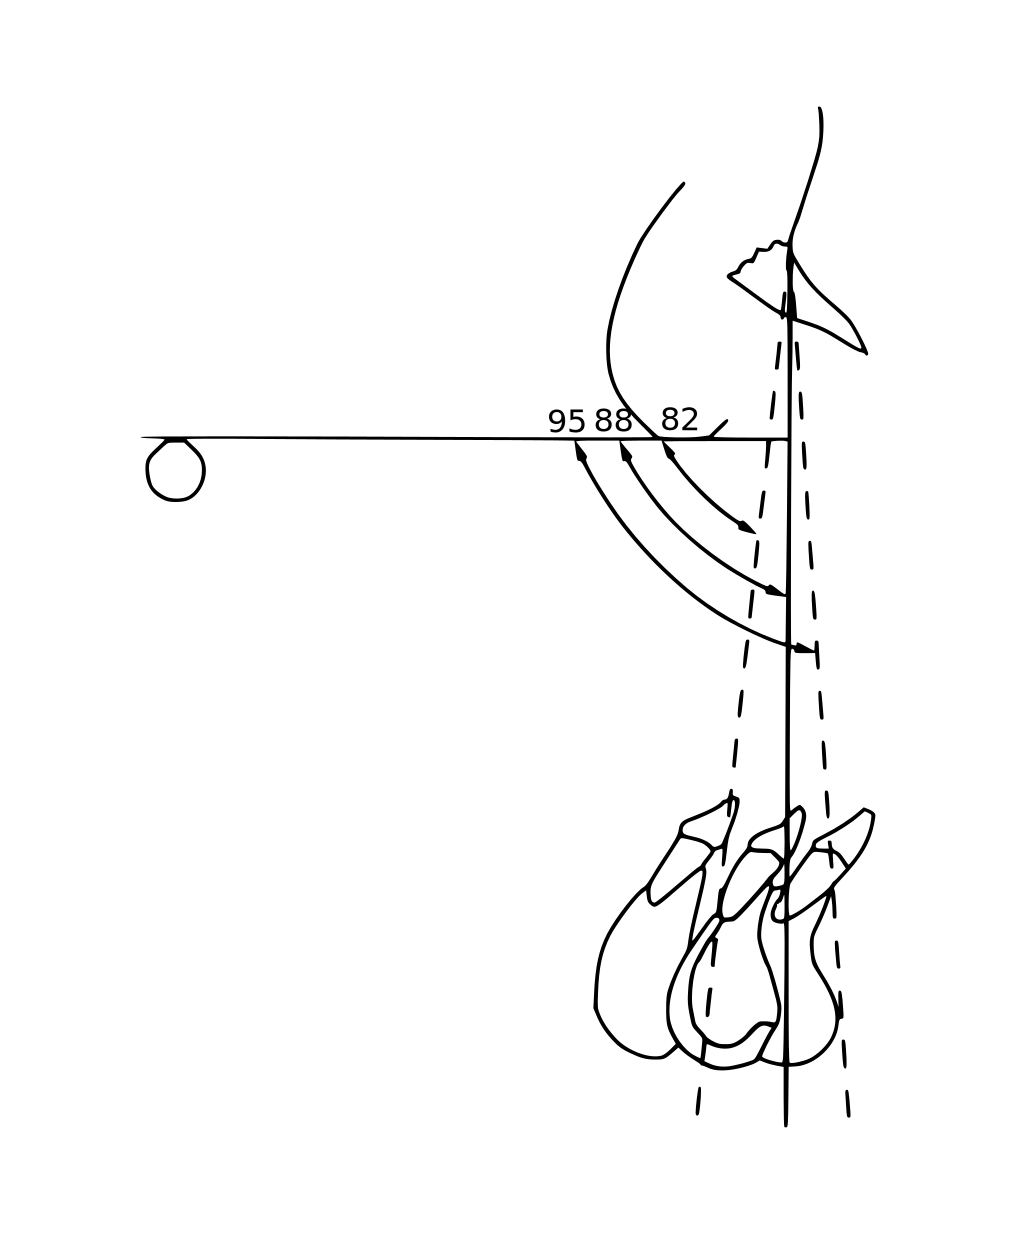
\includegraphics[width=.95\textwidth]{./images/downs_facciale.pdf}}
 \caption{Angolo facciale di Downs.}
 \label{fig:downs_facciale}
\end{minipage}\quad\quad
\begin{minipage}{.44\textwidth}
 \centering
 \fbox{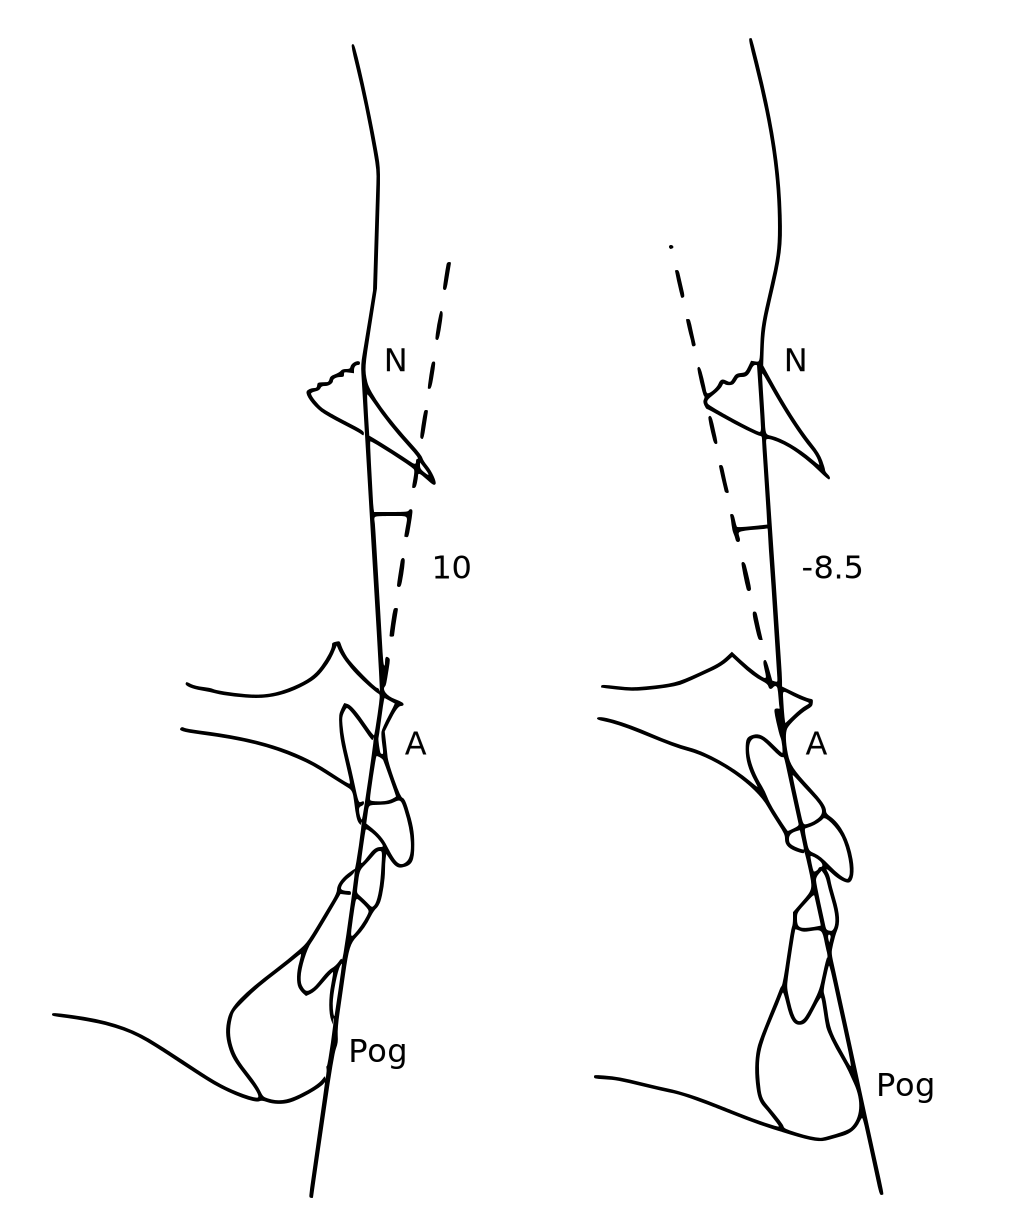
\includegraphics[width=.95\textwidth]{./images/downs_convessita.pdf}}
 \caption{Convessità facciale di Downs.}
 \label{fig:downs_convessita}
\end{minipage}
\end{figure}

\paragraph{Angolo facciale} (fig.~\ref{fig:downs_facciale}) usato per misurare il grado di retrusione o protrusione della mandibola. È l'angolo interno inferiore tra la linea facciale \piano{Na}{Pog} e il piano di Francoforte \textit{FH}. Ha un valore medio di 87.8 $\pm$ 3.6, con un range di normalità tra 82 e 95. Un mento prominente aumenta quest'angolo, un valore inferiore invece suggerisce una posizione retrusa del mento.

\paragraph{Convessità facciale} (fig.~\ref{fig:downs_convessita}) è un angolo formato dall'intersezione tra la linea \piano{Na}{A} e la linea \piano{A}{Pog}. Esso misura la relazione tra l'arco basale mascellare al suo limite anteriore (punto \punto{A}) e il profilo facciale totale (\piano{Na}{Pog}). Se la linea \piano{A}{Pog} tende in alto verso l'esterno, l'angolo è positivo. Un angolo positivo suggerisce una prominenza della base alveolare superiore rispetto alla mandibola. Un angolo negativo invece è associato ad un profilo prognatico. Il valore medio è di 0°, con un range di normalità tra -8.5° e 10°.

\paragraph{Piano \piano{A}{B}} (fig.~\vref{fig:downs_piano_ab}) forma un angolo con la linea \piano{Na}{Pog}, che indica la relazione tra i limiti anteriori dei processi alveolari e la linea facciale. Rappresenta una stima della difficoltà dell'ottenimento di una corretta inclinazione assiale e relazione tra gli incisivi dopo una terapia ortodontica. Poiché il punto \punto{B} è posizionato dietro il punto \punto{A}, quest'angolo è solitamente negativo, tranne che nelle Classi III o nelle Classi I con protrusione mandibolare. Un valore largamente negativo suggerisce una malocclusione di Classe II. Ha un valore medio di -4.6°, con un range di normalità tra -9° e 0°.

\begin{figure}[h!]
\centering
\begin{minipage}{.44\textwidth}
 \centering
 \fbox{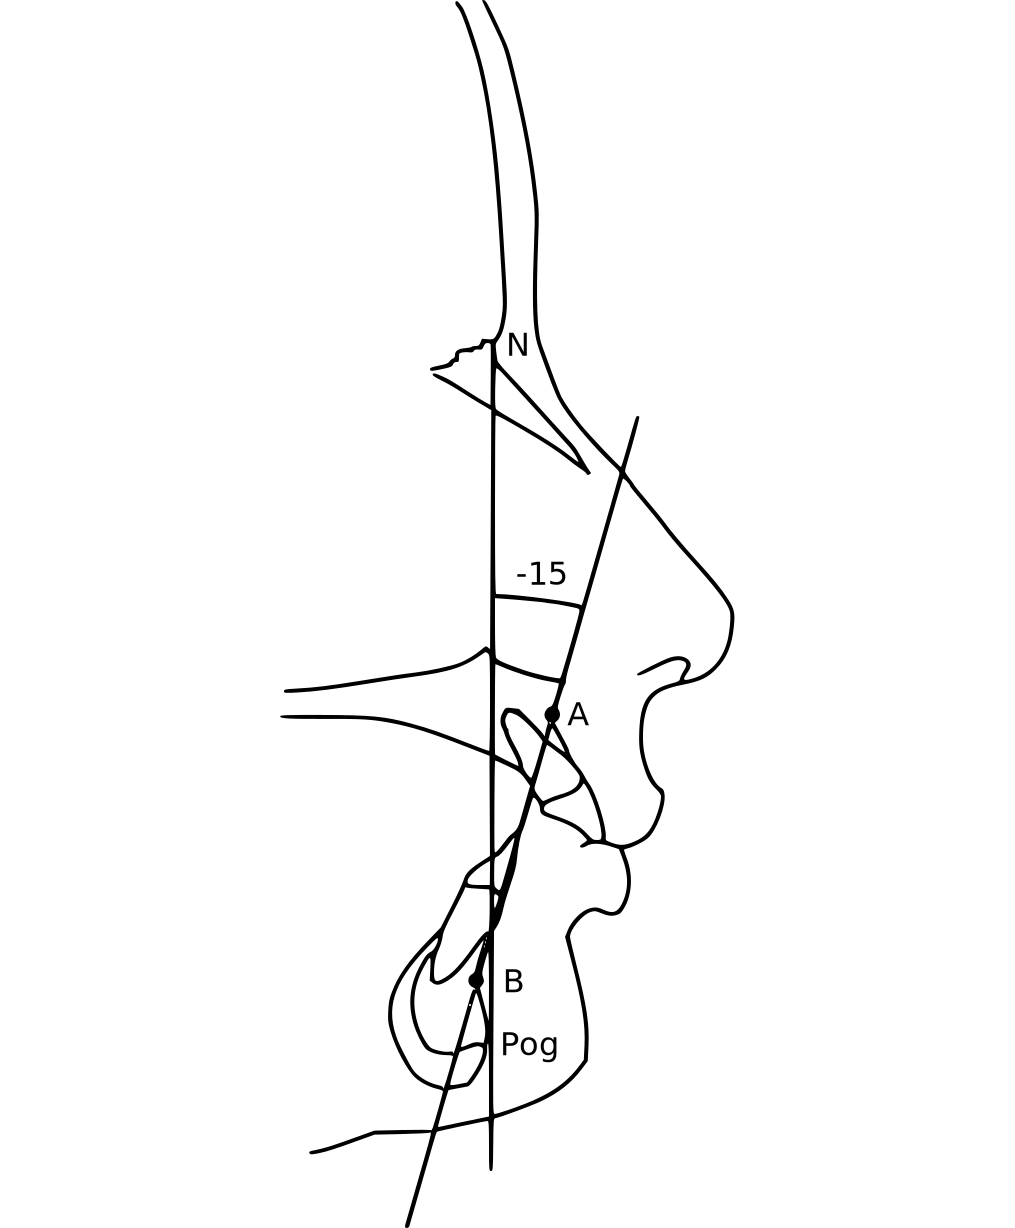
\includegraphics[width=.95\textwidth]{./images/downs_piano_ab.pdf}}
 \caption{Piano \piano{A}{B} di Downs.}
 \label{fig:downs_piano_ab}
\end{minipage}\quad\quad
\begin{minipage}{.44\textwidth}
 \centering
 \fbox{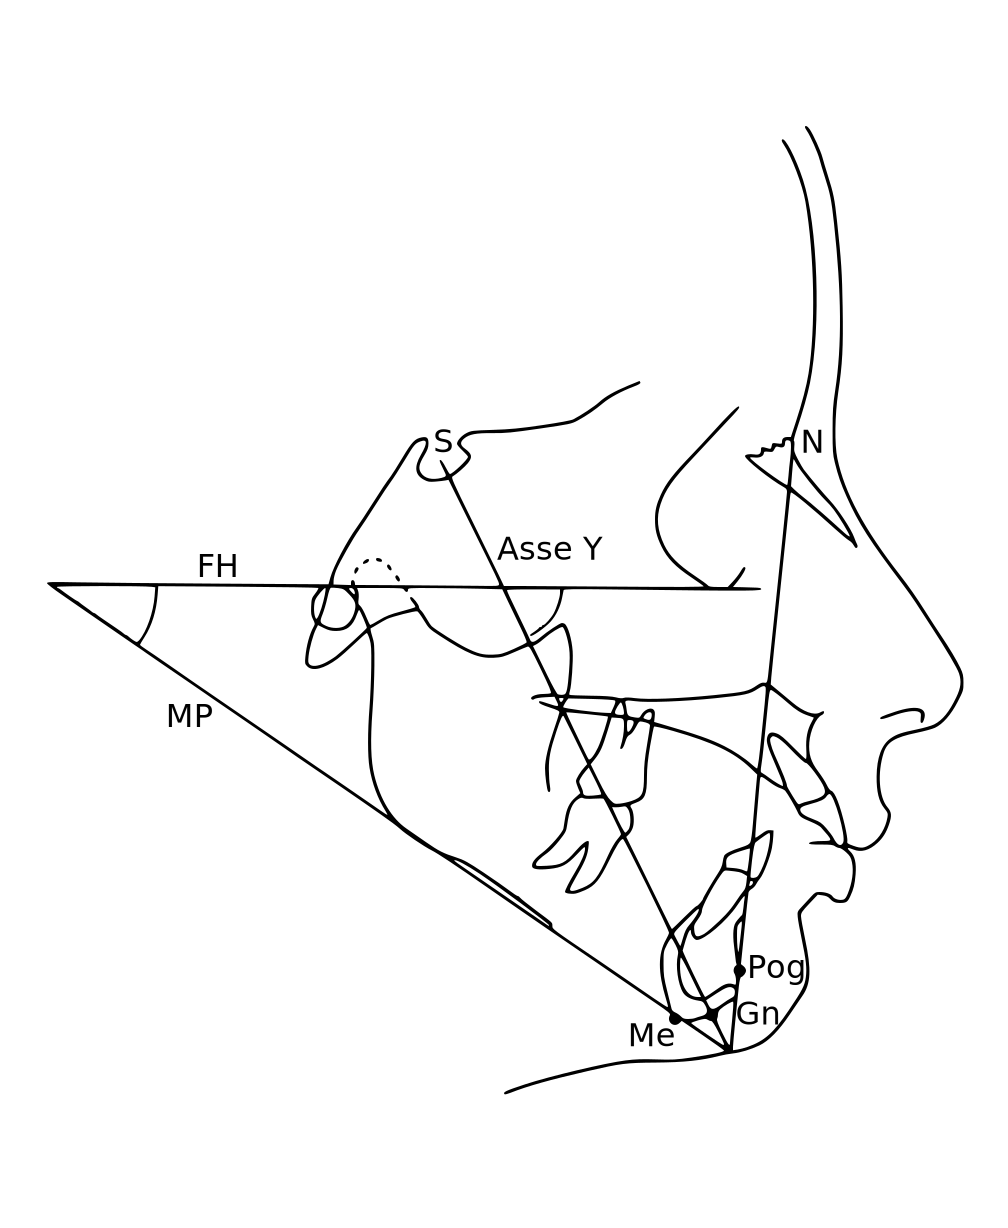
\includegraphics[width=.95\textwidth]{./images/downs_mandibolare_asse_y.pdf}}
 \caption{Piano mandibolare e Asse Y.}
 \label{fig:downs_mandibolare_asse_y}
\end{minipage}
\end{figure}

\paragraph{Piano mandibolare} (fig.~\vref{fig:downs_mandibolare_asse_y}) tangente all'angolo goniaco e al punto più inferiore della sinfisi mentoniera. L'angolo viene misurato dalla relazione tra il piano mandibolare e il piano di Francoforte. Si riscontrano valori elevati sia in soggetti retrusi e protrusi, e suggeriscono pattern facciali iperdivergenti, poco favorevoli al trattamento: essi risultano infatti complicati, con una prognosi incerta. Quest'angolo, però, non è sufficiente a indicare la natura della difficoltà che si potrà riscontrare durante il trattamento. Ha un valore medio di 21.9°, con un range di normalità tra 17° e 28°.

\paragraph{Asse Y} (fig.~\ref{fig:downs_mandibolare_asse_y}) rappresenta l'asse di crescita facciale, e indica la posizione in basso, o indietro, o in avanti del mento in relazione alla faccia superiore. Il relativo angolo è misurato all'intersezione della linea \piano{S}{Gn} e il piano di Francoforte. Quest'angolo è maggiore nelle Classi II rispetto alle Classi tendente-III. Un decremento di questo valore in radiografie seriali può essere interpretato come una crescita orizzontale prevalente su quella verticale. Ha un valore medio di 59.4°, con un range di normalità tra 53° e 66°.

\section{Misurazioni dentali}
\begin{table}[h]
%\footnotesize
\begin{tabularx}{\textwidth}{>{\bfseries}lXcc}
\toprule
 & Punti di riferimento & Val. medio & Range normalità \\
\cmidrule(r){2-4}
Piano occlusale (°) & \textit{PO} -- \textit{FH} & 9.3 & 1.5 -- 14 \\
Angolo interincisale (°) & assi inc. centrali & 135.4 & 130 -- 150.5 \\
Piano inc.-occlusale (°) & \textit{PO} -- asse inc. inf. & 14.5 $\pm$ 3.5 & 3.5 -- 20 \\
Piano inc.-mandibolare (°) & \textit{MP} -- asse inc. inf. & 1.4 & -8.5 -- 7 \\
Protr. inc. sup. (mm) & marg. inc. -- \piano{A}{Pog} & 2.7 & -1 -- 5 \\
\bottomrule
\end{tabularx}
\end{table}

\begin{figure}[h!]
 \centering
 \fbox{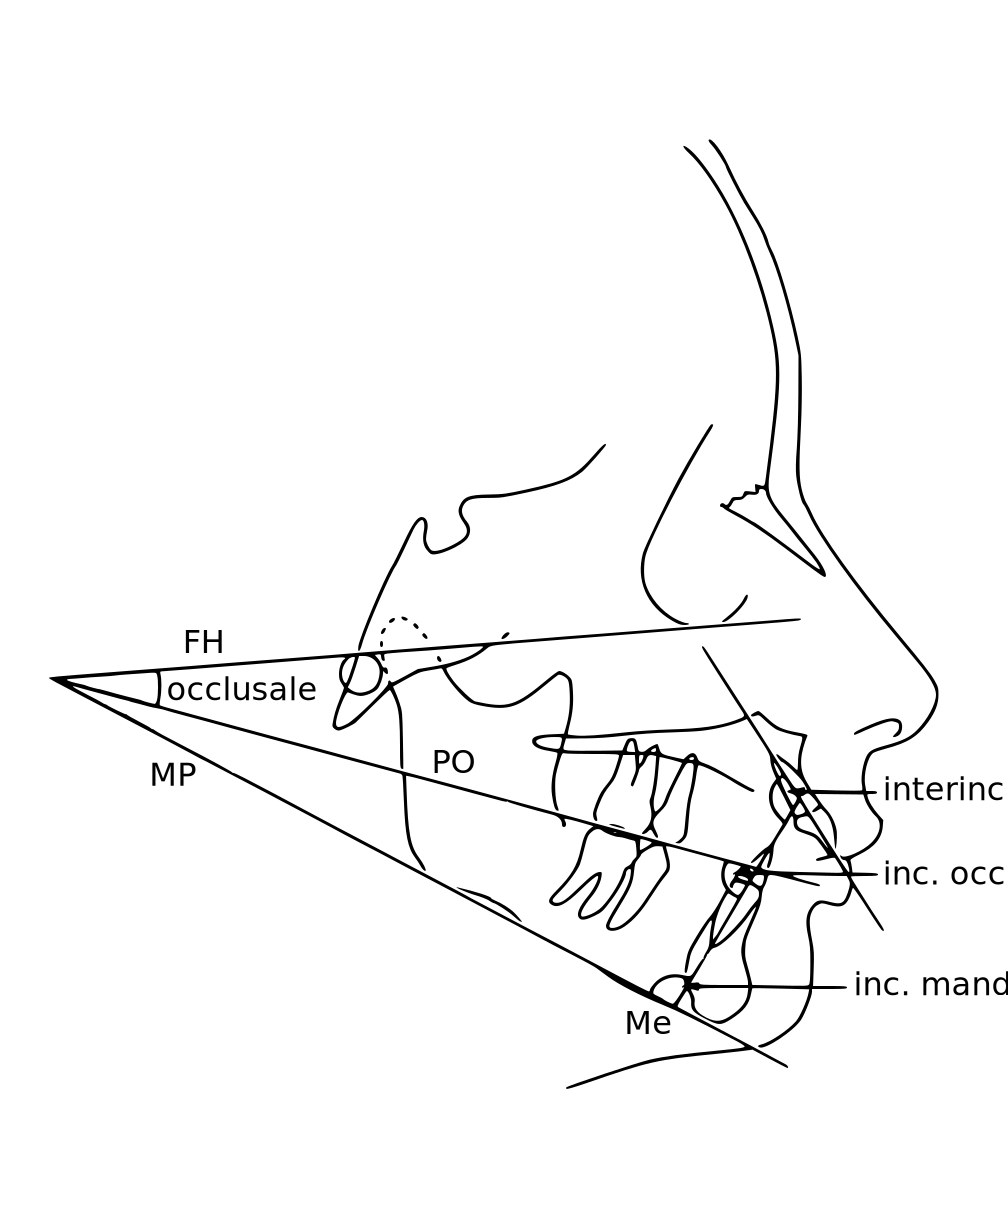
\includegraphics[width=.5\textwidth]{./images/downs_angoli_incisali_occlusale.pdf}}
 % downs_angoli_incisali_occlusale.pdf: 806x982 pixel, 72dpi, 28.43x34.64 cm, bb=0 0 806 982
 \caption{Angoli del piano occlusale, interincisale, incisivo-occlusale e incisivo-mandibolare.}
 \label{fig:downs_angoli_incisali_occlusale}
\end{figure}

\paragraph{Piano occlusale} (fig.~\ref{fig:downs_angoli_incisali_occlusale}) originariamente definito da Downs come la linea secante le cuspidi dei primi molari e l'overbite incisale. Nei casi di grossolana malposizione degli incisivi, Downs suggeriva di disegnare la linea secante le cuspidi dei primi molari e dei primi premolari. Il rispettivo angolo viene misurato tra il piano occlusale e il piano di Francoforte. Quando la parte anteriore del piano è posizionata più in basso rispetto alla parte posteriore, l'angolo è positivo. Angoli grandemente positivi si riscontrano in profili di Classe II, mentre risulta ridotto in casi di lunghi rami mandibolari. Ha un valore medio di 9.3°, con un range di normalità tra 1.5° e 14°.

\paragraph{Angolo interincisale} (fig.~\ref{fig:downs_angoli_incisali_occlusale}) viene stabilito tra gli assi maggiori degli incisivi centrali superiori ed inferiori. Ha un valore medio di 135.4°, con un range di normalità tra 130° e 150.5°.

\paragraph{Angolo piano incisivo-occlusale} (fig.~\ref{fig:downs_angoli_incisali_occlusale}) correla gli incisivi inferiori alla loro superficie lavorante. Viene misurato tra l'asse dell'incisivo inferiore e il piano occlusale, ha un valore medio di 14.5° $\pm$ 3.5°, con un range di normalità tra 3.5° e 20°.

\paragraph{Angolo piano incisivo-mandibolare} (fig.~\ref{fig:downs_angoli_incisali_occlusale}) è formato dall'intersezione del piano mandibolare con l'asse dell'incisivo inferiore. Quest'angolo è positivo quando gli incisivi sono inclinati in avanti rispetto al processo alveolare. Ha un valore medio di 1.4°, on un range di normalità tra -8.5° e 7°.

\begin{wrapfigure}{R}{.4\textwidth}
 \centering
 \fbox{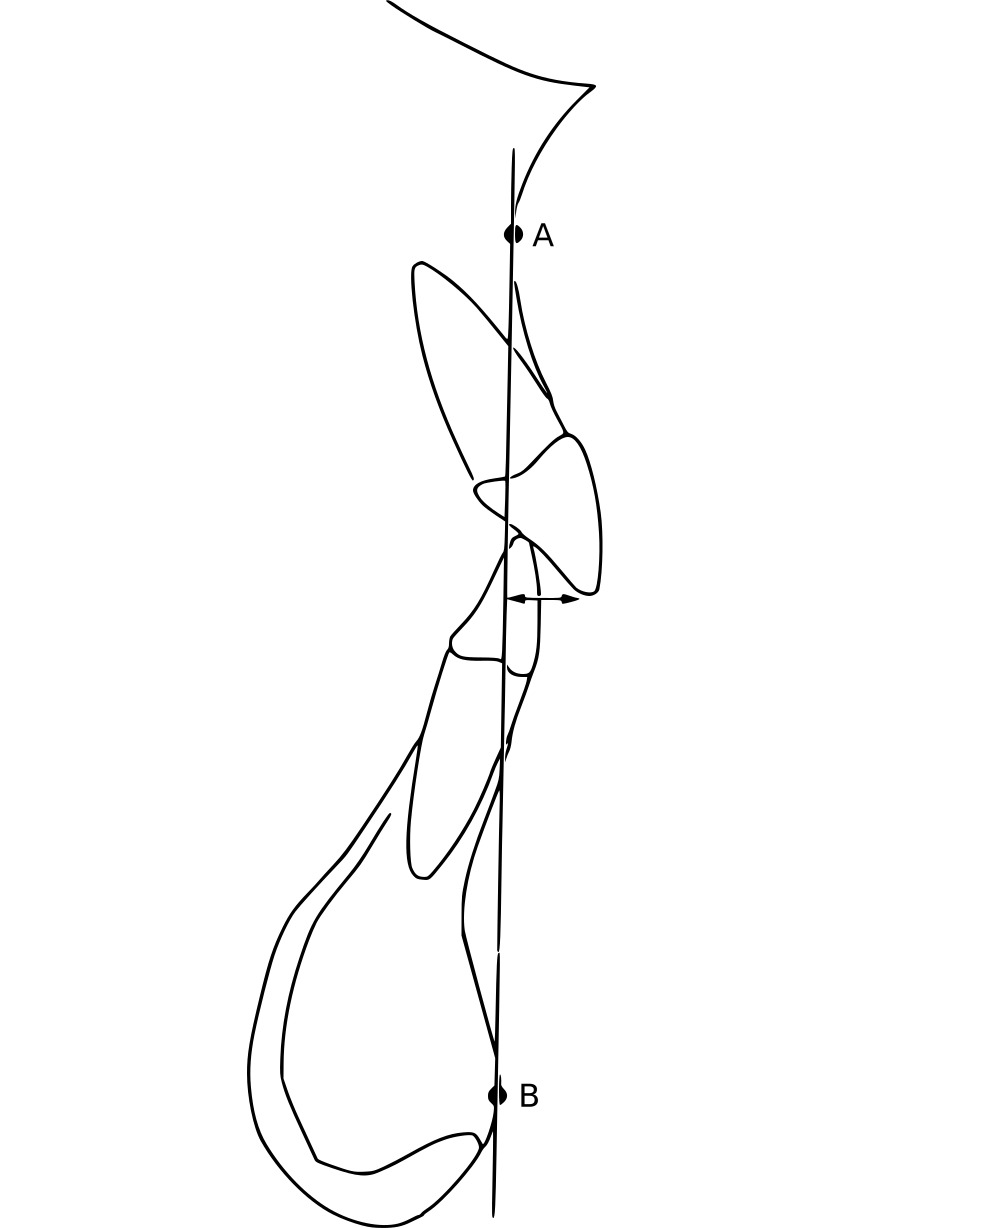
\includegraphics[width=.4\textwidth]{./images/downs_protrusione.pdf}}
 % downs_protrusione.pdf: 806x982 pixel, 72dpi, 28.43x34.64 cm, bb=0 0 806 982
 \caption{Protrusione incisivo superiore}
 \label{fig:downs_protrusione}
\end{wrapfigure}

\paragraph{Protrusione incisivi mascellari} (fig.~\ref{fig:downs_protrusione}) viene misurata in millimetri, come la distanza tra il margine incisale superiore e la linea \piano{A}{Pog}. La distanza è positiva se il margine incisale cade al davanti di tale linea, e indica la quantità di protrusione mascellare. Il valore medio è di 2.7mm, con un range di normalità tra -1mm e 5mm.

\chapter{Analisi di Steiner (secondo Giannì)}
\nocite{Steiner1953}

L'introduzione dell'analisi di Downs stimolò diversi ricercatori e clinici a sviluppare le proprie analisi: quello che ne seguì fu una proliferazione di marker cefalometrici che non fecero altro che confondere i clinici. Cecil C. Steiner selezionò quelli che per lui erano i parametri più significativi, e sviluppò un'analisi che credeva potesse fornire il massimo numero di informazioni cliniche con il minor numero di misurazioni.

Vennero quindi scelte alcune misure, e furono determinate delle medie statistiche su un numero di pazienti normo-occlusi.

Nell'analisi delle teleradiografie latero-laterali, Steiner propose la valutazione separata di varie parti del cranio, nello specifico i tessuti scheletrici, i tessuti dentali e i tessuti molli. L'analisi scheletrica si propone di porre in relazione la mascella e la mandibola tra di loro e con le ossa del cranio. L'analisi dentale mette in relazione gli incisivi superiori e inferiori con le rispettive basi ossee e tra di loro. Infine, l'analisi dei tessuti molli fornisce un mezzo per valutare il bilanciamento e l'armonia del profilo facciale inferiore\footcite{Steiner1953,Steiner1959,Steiner1960}.

A cavallo tra gli anni '70 e '80, Ennio Giannì\footcite{Gianni1980} propose diverse aggiunte all'analisi di Steiner. A tutt'oggi, questa è la tecnica più utilizzata, data la relativa semplicità e velocità d'esecuzione.

\begin{table}[h]
%\footnotesize
\caption{Punti specifici introdotti da Giannì}
\begin{tabularx}{\textwidth}{>{\textit}clX}
\toprule
%\multicolumn{3}{l}{\textbf{Punti di repere}} \\
%\midrule
D & Centro della sinfisi mentoniera & Punto di incontro del massimo diametro orizzontale con il massimo diametro verticale. \\
SOr & Sopraorbitario & Punto di incontro del tetto dell'orbita con il margine esterno dell'orbita stessa.\\
IST & Pavimento della sella & Il punto più basso del contorno della sella turcica. \\
\bottomrule
\end{tabularx}
\end{table}

\section{Analisi scheletrica}
\begin{table}[h]
%\footnotesize
\begin{tabularx}{\textwidth}{>{\bfseries}lXc}
\toprule
 & Punti di riferimento & Valore medio\\
\cmidrule(r){2-3}
Angolo \angolo{SNA} &  & 82° $\pm$ 2° \\
Angolo \angolo{SNB} &  & 80° $\pm$ 2° \\
Angolo \angolo{ANB} &  & 2° $\pm$ 2° \\
Angolo cranio-spinale & piano \piano{S}{N} -- piano bispinale & 10° $\pm$ 3° \\
Angolo cranio-occlusale & piano occlusale -- \piano{S}{N} & 14° $\pm$ 3° \\
Angolo cranio-mandibolare & piano mandibolare -- \piano{S}{N} & 32° $\pm$ 5° \\
Angolo intermascellare & piano bispinale -- piano mandib. & 20° $\pm$ 5° \\
Angolo occluso-spinale & piano occlusale -- piano bispinale & 8° $\pm$ 2° \\
Angolo occluso-mandibolare & piano occlusale -- piano occlusale & 12° $\pm$ 3° \\
Base cranica posteriore & piano \piano{S}{N} -- piano \piano{S}{Ba} & 129° $\pm$ 5° \\
Angolo cranio-sinfisario & piano \piano{S}{N} -- piano \piano{N}{D} & 76° $\pm$ 3° \\
\bottomrule
\end{tabularx}
\end{table}

Nelle analisi antropologiche tradizionali, così come nell'analisi di Downs, il piano di riferimento era il \textit{piano di Francoforte}. Sulle teleradiografie latero-laterali è però spesso difficile identificare i punti Porion e Orbitale, per la determinazione di tale piano. Steiner scelse quindi la \textbf{base cranica anteriore} (Sella-Nasion) come piano di riferimento della sua analisi. Il vantaggio di utilizzare due punti ``mediani'' è che si muovono minimamente quando la testa devia dalla posizione di profilo, o quando la testa ruota nel cefalostato.

\begin{figure}[p!]
\subfloat[][]
   {\label{fig:steiner_sna}\fbox{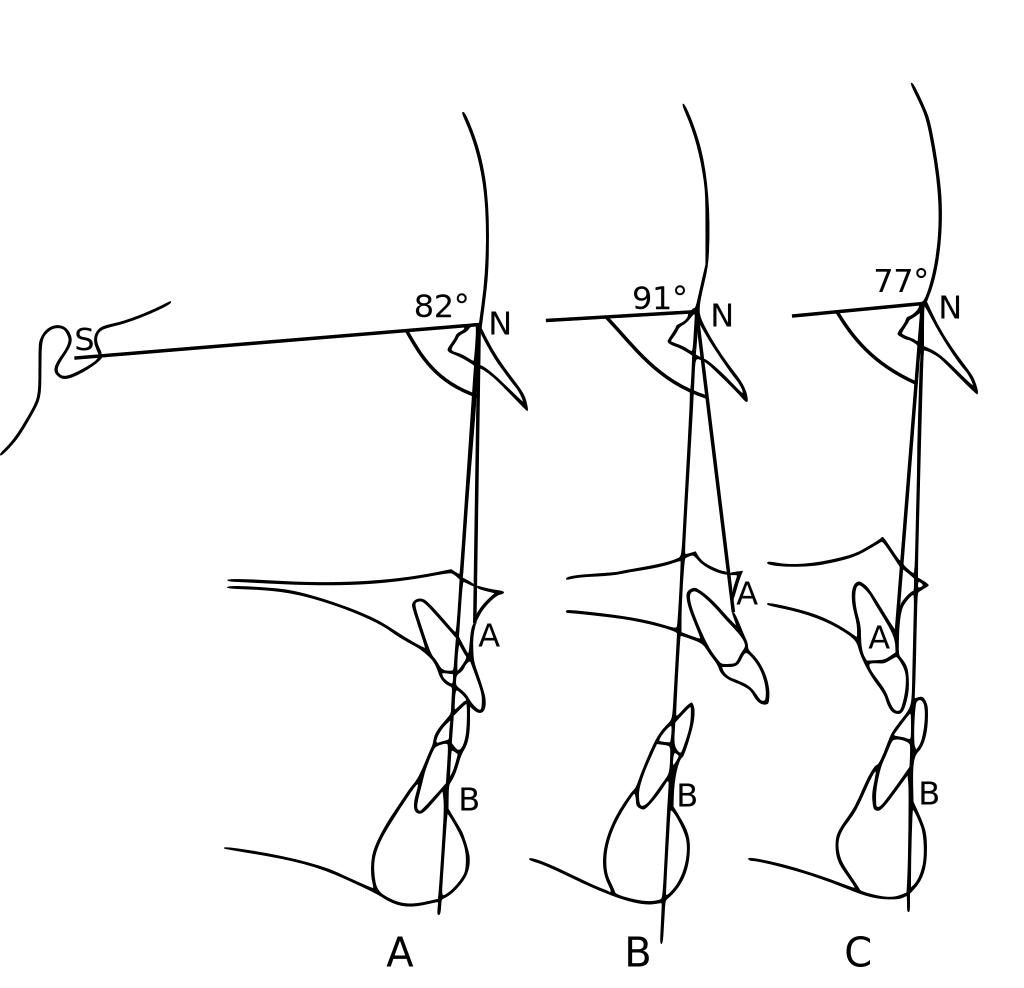
\includegraphics[width=.45\textwidth]{./images/steiner_sna.pdf}}} \quad
\subfloat[][]
   {\label{fig:steiner_snb}\fbox{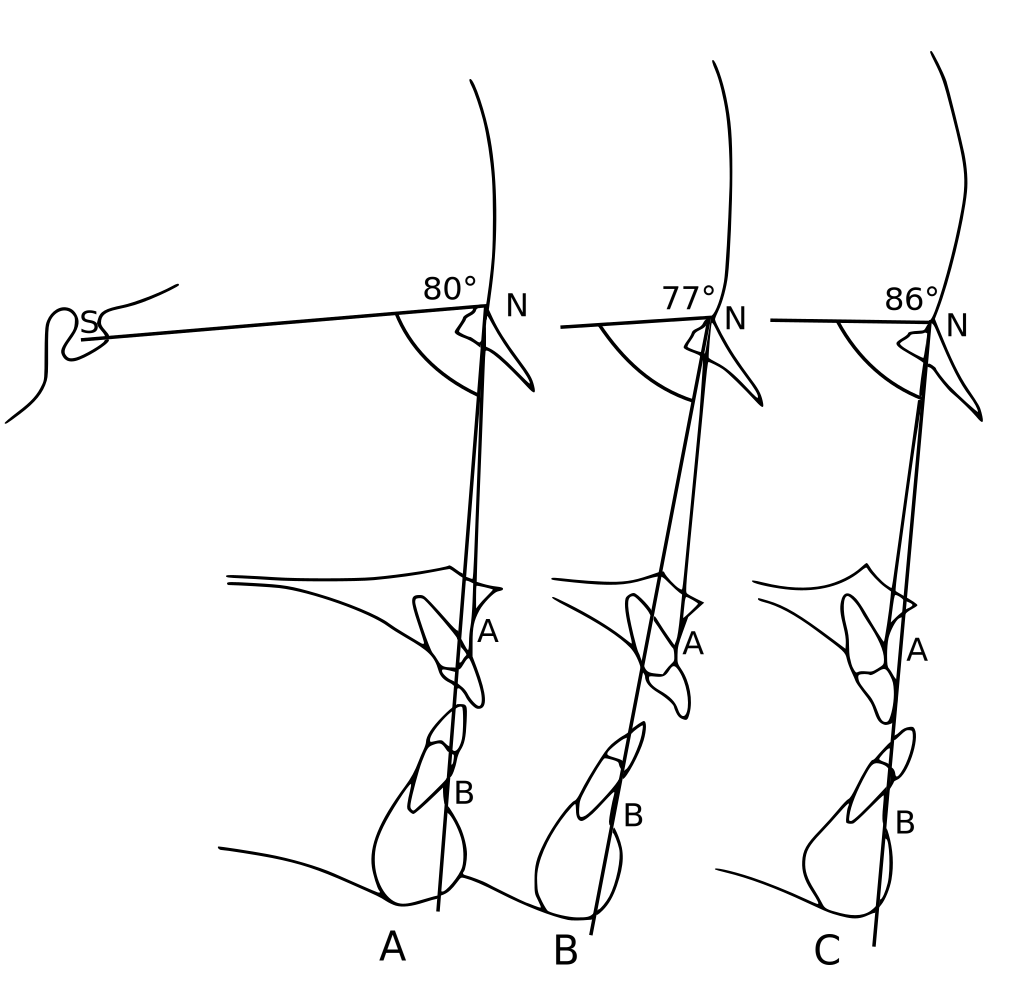
\includegraphics[width=.45\textwidth]{./images/steiner_snb.pdf}}}
 \centering
 % steiner_sna.jpg: 1024x988 pixel, 72dpi, 36.12x34.85 cm, bb=0 0 1024 988
 \caption{\subref{fig:steiner_sna} \angolo{SNA}: profilo normale, profilo retruso, profilo protruso. \subref{fig:steiner_snb} \angolo{SNB}: profilo normale, profilo retruso, profilo protruso.}
 \label{fig:steiner_sna_snb}
\end{figure}
\begin{figure}[p!]
 \centering
 \fbox{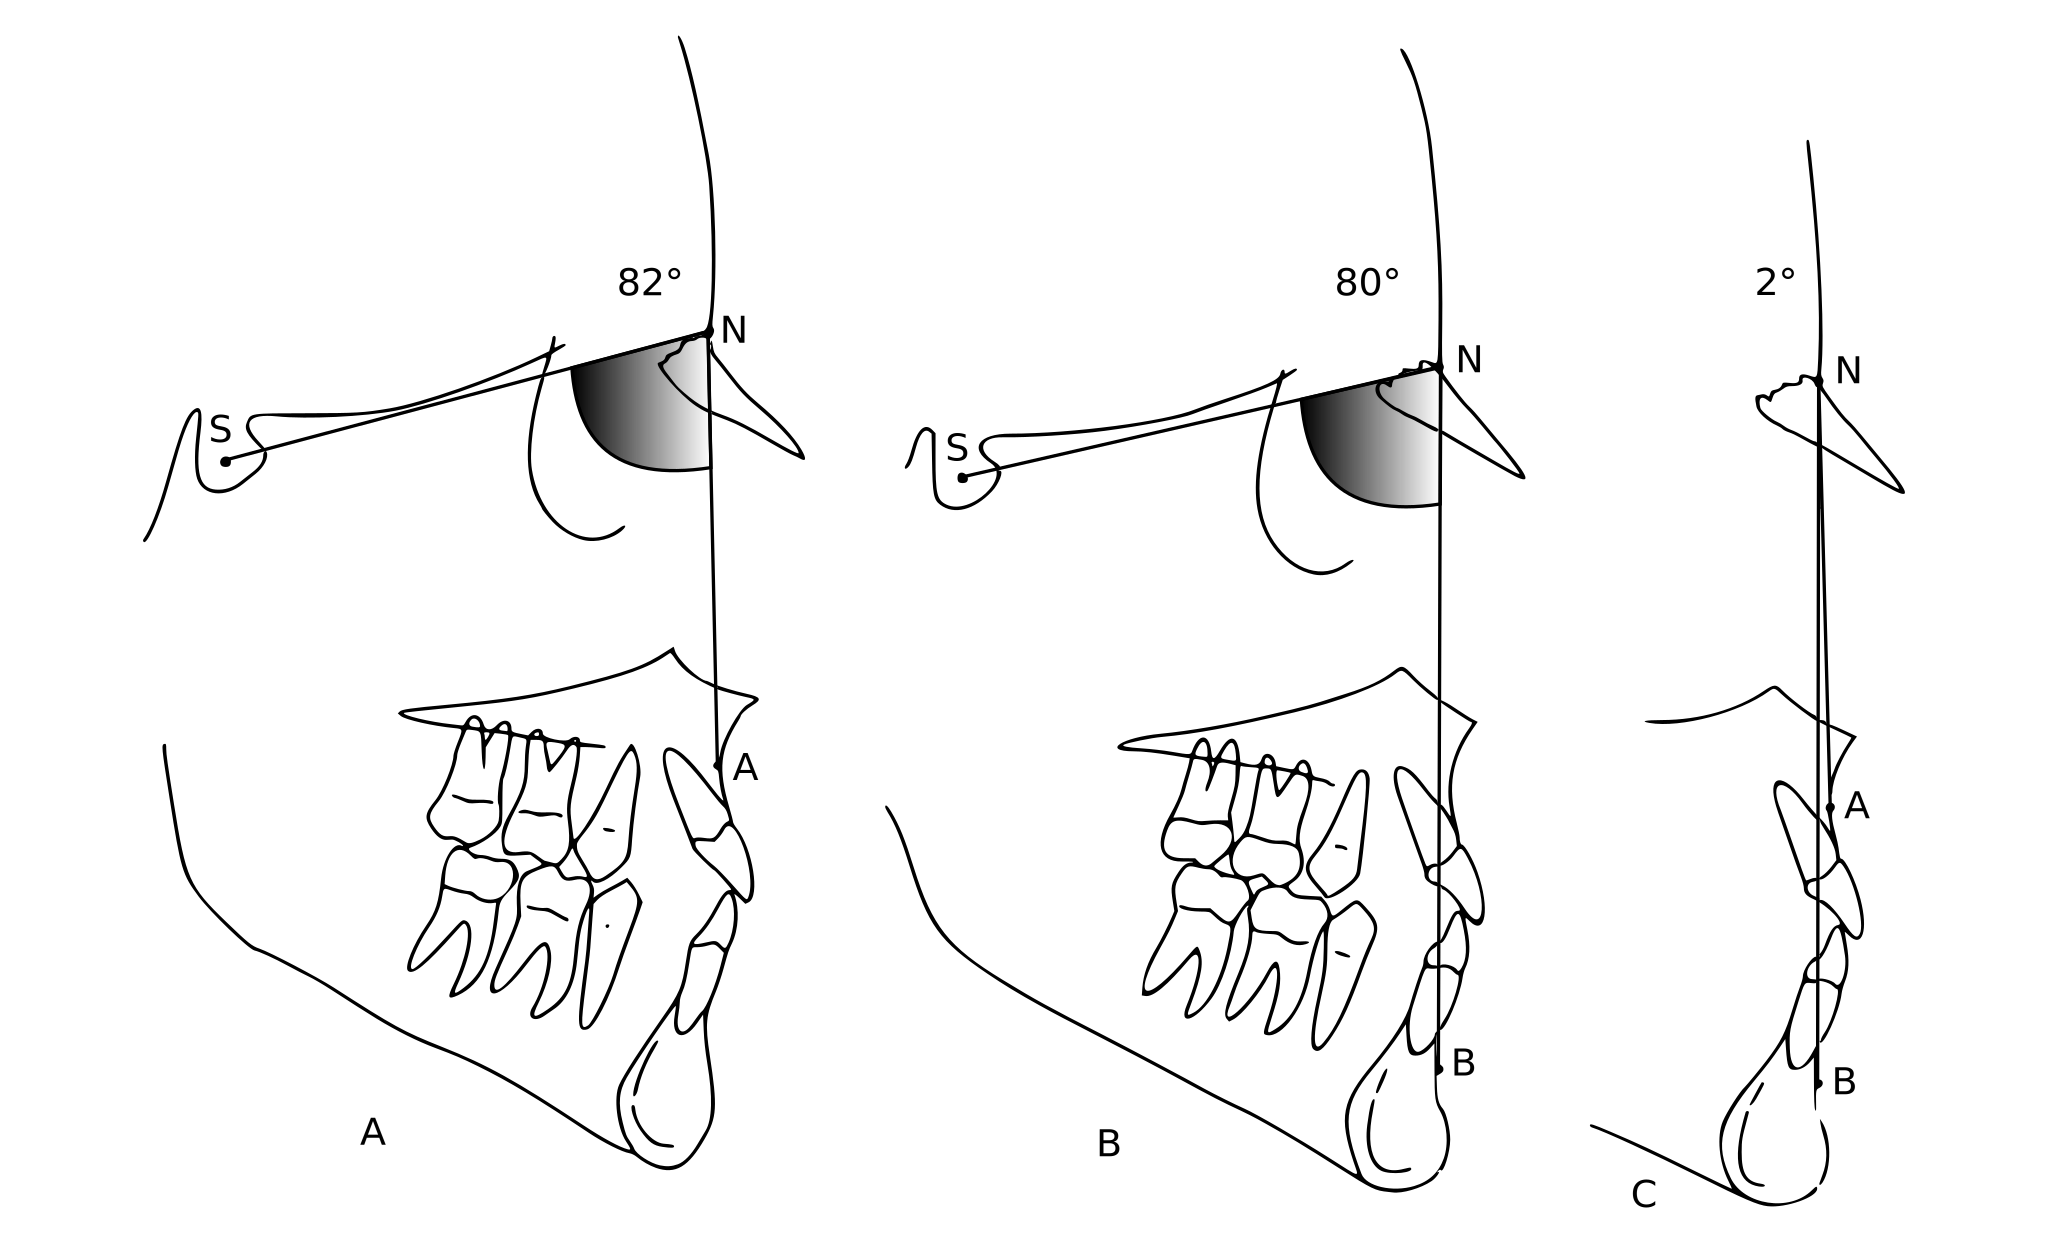
\includegraphics[width=.9\textwidth]{./images/steiner_anb.pdf}}
 % steiner_anb.jpg: 2152x1306 pixel, 72dpi, 75.92x46.07 cm, bb=0 0 2152 1306
 \caption{l'angolo interincisale \angolo{ANB} è dato dalla differenza tra \angolo{SNA} e \angolo{SNB}.}
 \label{fig:steiner_anb}
\end{figure}

\paragraph{Mascella (angolo \angolo{SNA})}
I punti A e B vengono considerati come i limiti anteriori delle basi apicali di, rispettivamente, mascella e mandibola. Perciò, per determinare la posizione della mascella rispetto alla base cranica, viene calcolato l'angolo \angolo{SNA}, il cui valore medio è 82° $\pm$ 2° (fig.~\vref{fig:steiner_sna}). Se il valore angolare è maggiore, la mascella si trova in posizione anteriore rispetto alla base cranica. Di contro, se il valore inferiore, la mascella si troverà posizionata posteriormente.

\paragraph{Mandibola (angolo \angolo{SNB})}
Per valutare la posizione della mandibola, viene calcolato l'angolo \angolo{SNB} (valore medio 80° $\pm$ 2°, fig.~\ref{fig:steiner_snb}). Un angolo minore indica una mandibola retrusa, un angolo maggiore indica una mandibola protrusa.

\paragraph{Relazione tra mascella e mandibola (\angolo{ANB})}
Valutando i valori \angolo{SNA} e \angolo{SNB}, solitamente è possibile riconoscere il segmento osseo malposizionato. Il valore più significativo è, comunque, l'angolo \angolo{ANB}, che fornisce informazioni sulla posizione dei due segmenti ossei uno relativo all'altro (fig.~\vref{fig:steiner_anb}).

Steiner sosteneva come \angolo{SNA} non fosse importante quanto \angolo{SNB} e \angolo{ANB}, in quanto indica solamente una retrusione o protrusione rispetto alla base del cranio. Piuttosto, è più importante la discrepanza tra mascella e mandibola. Il valore medio dell'angolo \angolo{ANB} è di 2° $\pm$ 2°: un valore maggiore indica una \textit{tendenza} alla \textit{Classe II scheletrica}, e più è grande questo valore, più difficile sarà correggere la malocclusione. Valori minori dell'angolo, e valori sotto lo zero, indicano che la mandibola è protrusa rispetto alla mascella, suggerendo una \textit{Classe III scheletrica}.

\paragraph{Angolo cranio-spinale} considerato da Giannì, rappresenta l'inclinazione del mascellare superiore nei confronti della base del cranio. È l'angolo compreso tra il piano \piano{S}{Na} e il piano bispinale \piano{SNA}{SNP}. Ha un valore medio di 10° $\pm$ 3°. Valori minori depongono per un'antero-rotazione del piano bispinale: il punto \punto{A} tende a portarsi verso l'alto e in avanti. Viceversa, valori maggiori segnalano una post-rotazione del piano bispinale, con uno spostamento in basso e indietro del punto \punto{A}. La rotazione del piano bispinale, se considerata in relazione al piano mandibolare, influenza la divergenza intermascellare, con una variazione dell'angolo \angolo{ANB}.

\paragraph{Angolo cranio-occlusale} compreso tra il piano \piano{S}{Na} e il piano occlusale. Ha un valore medio di 14° $\pm$ 3°; una minore o maggiore apertura indica, rispettivamente, una antero- e una post-rotazione del piano occlusale. Tale angolo ha importanza in corso di terapia intercettiva: un'antero-rotazione occlusale, infatti, favorisce il trattamento di una Classe II scheletrica da retrusione mandibolare, ma è sfavorevole al ripristino di una Classe III da protrusione mandibolare. Viceversa per la post-rotazione, in quanto rappresenta un ostacolo all'avanzamento della mandibola.

\paragraph{Angolo cranio-mandibolare} rappresenta l'in\-cli\-na\-zio\-ne della mandibola rispetto alla base del cranio. È l'angolo compreso tra il piano \piano{S}{Na} e il piano mandibolare \piano{Go}{Gn}. Ha un valore medio di 32° $\pm$ 5°; valori minori o maggiori indicano, rispettivamente, un'antero- o una post-rotazione del piano mandibolare, con tendenze rispettivamente ipo- e iper-divergenti.

\paragraph{Angolo intermascellare} considerato anche questo da Giannì, e quindi non presente nell'analisi proposta originariamente da Steiner, evidenzia l'inclinazione, sul piano sagittale, delle basi mascellari tra di loro. È dato dall'incontro del piano bispinale \piano{SNA}{SNP} con il piano mandibolare \piano{Go}{Gn}. Ha un valore medio di 20° $\pm$ 5°: soggetti rientranti entro questo valore vengono definiti \textit{mesodivergenti}; valori superiori definiscono gli \textit{iperdivergenti}, valori inferiori i soggetti \textit{ipodivergenti}. Tali squilibri possono derivare da rotazioni varie del piano bispinale o dal piano mandibolare: si ha iperdivergenza in caso di post-rotazione del piano mandibolare, oppure antero-rotazione del piano bispinale, oppure una combinazione di entrambi. Lo stesso avviene nel caso dell'ipodivergenza: antero-rotazione mandibolare, post-rotazione del piano bispinale, o una combinazione di essi.

\paragraph{Angolo occluso-spinale e occluso-mandibolare} proposti da Giannì, sono formati dal piano occlusale con, rispettivamente, il piano bispinale e il piano occlusale. Il valore medio per il primo è di 8° $\pm$ 2°, per il secondo 12° $\pm$ 3°.

\paragraph{Angolo della base cranica posteriore} anche questo proposto da Giannì, è formato dal piano \piano{S}{Na} e il piano sfeno-occipitale \piano{S}{Ba}. Esso ci informa sulla direzione di crescita dell'articolazione temporo-mandibolare\nocite{Ricketts1960}. Ha un valore medio di 129° $\pm$ 5°, e aumenta di un grado all'anno fino alla fine della fase dinamica di crescita. Valori maggiori indicano che la cavità glenoidea è in posizione alta ed arrestrata, che a sua volta indica una impostazione distale della mandibola: questo è un elemento sfavorevole alla correzione delle seconde classi scheletriche mandibolari.

\paragraph{Angolo cranio-sinfisario} introdotto da Giannì, è formato dal piano craniale \piano{S}{N} con il piano \piano{N}{D}. Il punto \punto{D} è definito da Giannì come il \textit{centro geometrico della sinfisi mentoniera}, ossia il punto d'incontro del massimo diametro verticale con il massimo diametro orizzontale -- similarmente al punto \punto{S} per la sella turcica. Quest'angolo evidenzia, analogamente all'angolo \angolo{SNB}, la situazione della mandibola nei confronti della base cranica. Ha un valore medio di 76° $\pm$ 3°.

\paragraph{Dimensioni sagittali della mandibola} analizzate da Giannì ai fini dell'evidenziazione di una normo-, iper- o ipo-mandibolia, Giannì considera il rapporto dimensionale tra la lunghezza del corpo mandibolare (\piano{Go}{Me}) e la lunghezza della base del cranio (\piano{S}{N}). Da 6 a 12 anni la lunghezza della base cranica aumenta di 1mm l'anno, la mandibola invece da 1,5mm a 2mm l'anno. A 12 anni, indipendentemente dal sesso, il rapporto lineare tra \piano{S}{N} e \piano{Go}{Me} è di 1:1. Superata questa età, il rapporto si mantiene costante nella donna, mentre nell'uomo si modifica a vantaggio della mandibola.

\paragraph{Dimensioni sagittali della mascella} secondo Giannì, è la distanza lineare tra \punto{SNP} e \punto{A}. All'età di 4 anni, nella crescita ortognatica, tale distanza è di 41mm, con una crescita di 0,5mm per anno fino ad un massimo di 46mm a crescita terminata. Un aumento o una diminuzione di tale valore depone per la presenza di una iper- o ipo-maxillia.

\paragraph{Rapporto tra base cranica posteriore e ramo mandibolare} (Giannì) A 12 anni di età, nella crescita ortognatica, il rapporto tra la base cranica posteriore, definita come \piano{S}{Ar}, e il ramo mandibolare, definito come \piano{Ar}{Go}, è di 2:3. Una variazione del rapporto verso valori più bassi depone per una ipoplasia della branca montante della mandibola, che aggrava la crescita in post-rotazione. Al contrario, un rapporto aumentato depone per un ramo mandibolare lungo, che può compensare una crescita in post-rotazione.

\paragraph{Dimensioni verticali scheletriche anteriori} (Giannì) viene preso in considerazione il triangolo \punto{SOr}-\punto{SNA}-\punto{Me}. La distanza \piano{SOr}{SNA}, la distanza \piano{SNA}{Me} e la distanza \piano{SOr}{Me} rappresentano, rispettivamente, la dimensione verticale scheletrica anteriore superiore, inferiore e totale.

Tra la misura superiore e quella inferiore esiste un rapporto definito di crescita in armonia con l'età e con il sesso. A 4 anni di età, la dimensione scheletrica anteriore superiore è uguale a quella inferiore. Successivamente, fino a 12 anni, tale rapporto si modifica a favore del tratto inferiore (crescita differenziale di 0,7mm annui). A 12 anni, quindi, la misura scheletrica antero-superiore è uguale a quella antero-inferiore + 5,6mm. Dopo i 12 anni, la crescita subisce variazioni in base al sesso: nella donna, la differenza tra le due misure rimane costante (5,6mm); nell'uomo, invece, la crescita differenziale continua, pertanto a 20 anni la differenza tra le due misure sarà di 11,2mm. Secondo queste misurazioni, Giannì individua tre classi scheletriche sul piano verticale:

\begin{itemize}
\item \textbf{normoverti-bite scheletrico} (I classe scheletrica verticale), quando i rapporti tra la misura antero-superiore e antero-inferiore collimano con i valori sopra esposti;
\item \textbf{open-bite scheletrico} (II classe scheletrica verticale), quando la dimensione scheletrica antero-inferiore aumenta eccessivamente rispetto alla dimensione antero-superiore;
\item \textbf{deep-bite scheletrico} (III classe scheletrica verticale), quando la dimensione scheletrica antero-inferiore diminuisce eccessivamente, al di là dei valori nella media.
\end{itemize}

Queste classi non devono essere confuse con il normoverti-bite, l'open-bite e il deep-bite dentario. Da un punto di vista clinico, infatti, non sempre esiste armonia tra la classe scheletrica verticale e la classe dentaria verticale.

\paragraph{Dimensioni verticali scheletriche posteriori} (Giannì) viene preso in considerazione il triangolo \punto{IST}-\punto{SNP}-\punto{Go}. Similarmente alle dimensioni verticali scheletriche anteriori, anche qui si considerano le varie misure \piano{IST}{SNP}, \piano{SNP}{Go}, \piano{IST}{Go} (rispettivamente, dimensione postero-superiore, postero-inferiore, posteriore totale).

Nella crescita ortognatica, la crescita delle dimensioni verticali scheletriche posteriori prevale su quella delle parti anteriori: tale dinamica è alla base del movimento di antero-rotazione. Il rapporto tra le due misure è del 62\% (secondo Jarabak e Fizzel): tale rapporto aumenta nella crescita orizzontale, e diminuisce nella crescita in post-rotazione.

\begin{wrapfigure}{R}{.4\textwidth}
 \centering
 \fbox{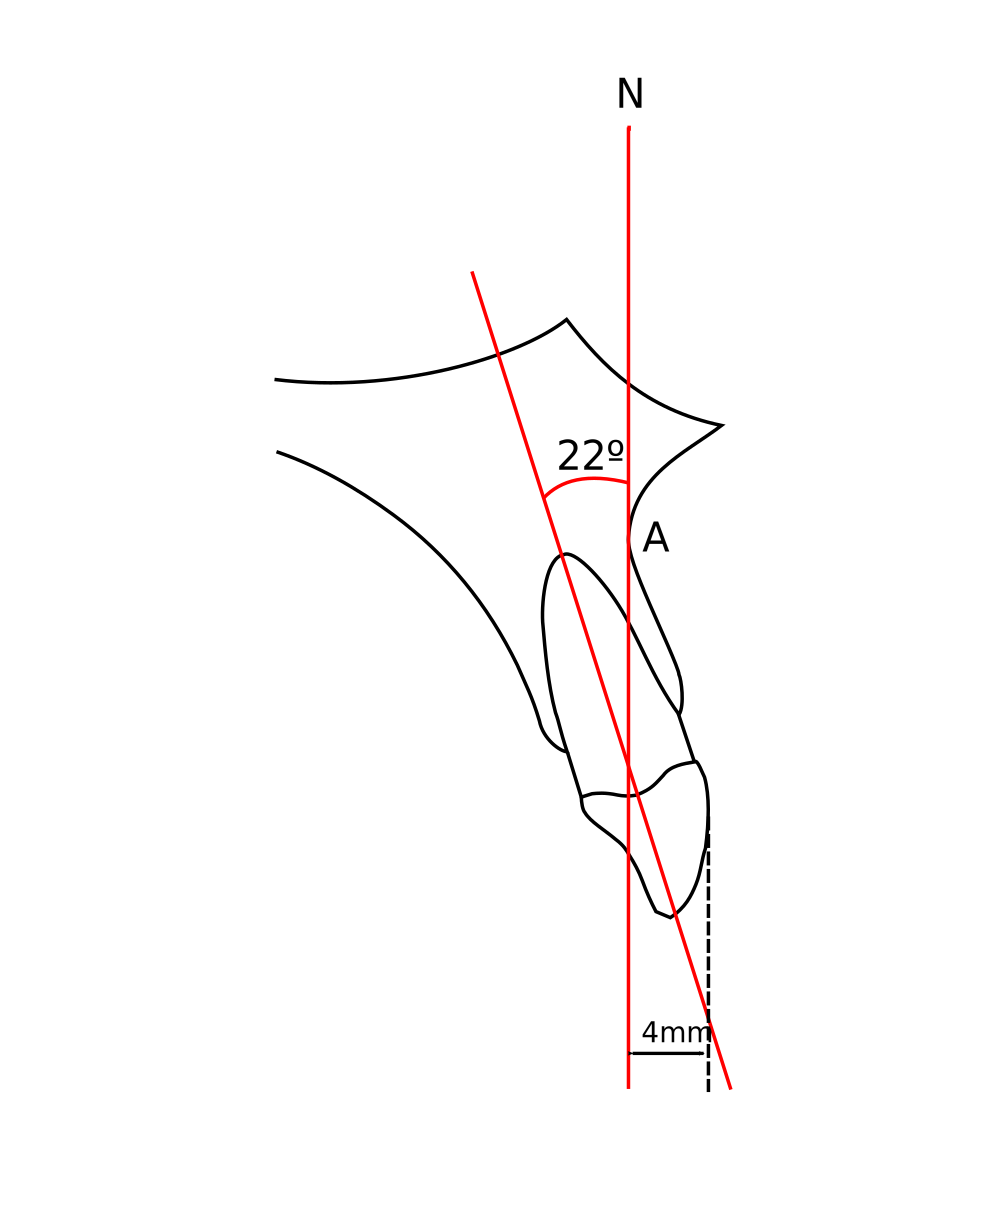
\includegraphics[width=.4\textwidth]{./images/steiner_incisale.pdf}}
 % steiner_incisale.jpg: 1006x1227 pixel, 72dpi, 35.49x43.29 cm, bb=0 0 1006 1227
 \caption{Posizione e angolazione ``ideale'' dell'incisivo superiore secondo Steiner}
 \label{fig:steiner_incisivo_superiore}
\end{wrapfigure}

\section{Analisi dentale}
\begin{table}[h]
%\footnotesize
\begin{tabularx}{\textwidth}{>{\bfseries}lXc}
\toprule
 & Punti di riferimento & Valore medio \\
\cmidrule(r){2-3}
Ang. occl.-inc. sup. & piano occlusale -- asse maggiore inc. sup. & 60° $\pm$ 2° \\
Inclinaz. inc. sup. & \piano{N}{A} -- asse maggiore inc. sup. & 22° \\
Posiz. inc. sup. & \piano{N}{A} -- superficie labiale inc. sup. & 4mm \\
Ang. occl.-inc. inf. & piano occlusale -- asse maggiore inc. inf. & 70° $\pm$ 3° \\
Inclinaz. inc. inf. & \piano{N}{B} -- asse maggiore inc. inf. & 25° \\
Posiz. inc. inf. & \piano{N}{B} -- superficie labiale inc. inf. & 4mm \\
Angolo interincis. & assi maggiori incisivi & 130° $\pm$ 5° \\
Angolo occl.-mol. sup. & piano occlusale -- asse maggiore sesto sup. & 90° $\pm$ 3° \\
%Angolo bimolare inf. & assi maggiori settimo e ottavo inf. & < 10° \\
\bottomrule
\end{tabularx}
\end{table}

Solitamente l'analisi dentale serve a confermare le valutazioni cliniche già compiute. D'altro canto, esistono numerosi casi in cui le valutazioni radiografiche differiscono notevolmente da quelle cliniche.

\paragraph{Posizione incisivo superiore}
La posizione degli incisivi superiori viene determinata correlando i denti alla linea \punto{N}-\punto{A}. È possibile considerare due valori: il primo riguarda l'angolazione dell'asse del dente e viene calcolato misurando il valore in gradi dell'angolo tra \punto{N}-\punto{A} e l'asse del dente. Il secondo valuta il posizionamento relativo, misurato in millimetri tra \punto{N}-\punto{A} e la superficie più labiale.

Usando questo metodo, gli incisivi centrali superiori dovrebbero essere posizionati in modo tale da avere la superficie più labiale ad una distanza di 4mm dalla linea, e un'inclinazione di 22°.

La sola valutazione dell'angolazione dell'incisivo superiore non è infatti sufficiente a dare un giudizio sulla posizione dei denti: potrebbe infatti capitare che l'angolazione sia corretta, ma che il dente sia traslato in avanti o indietro rispetto alla linea \punto{N}-\punto{A} (fig.~\ref{fig:steiner_traslazione}).

Allo stesso modo, la sola rilevazione della distanza millimetrica della superficie più labiale non è sufficiente. Non è difficile immaginare un incisivo a 4mm di distanza, ma inclinato diversamente (fig.~\ref{fig:steiner_rotazione}).

Giannì introdusse un ulteriore angolo, in rapporto al piano occlusale, con un valore medio di 60° $\pm$ 2°.

\begin{figure}[p!]
\subfloat[][]
   {\label{fig:steiner_traslazione}\fbox{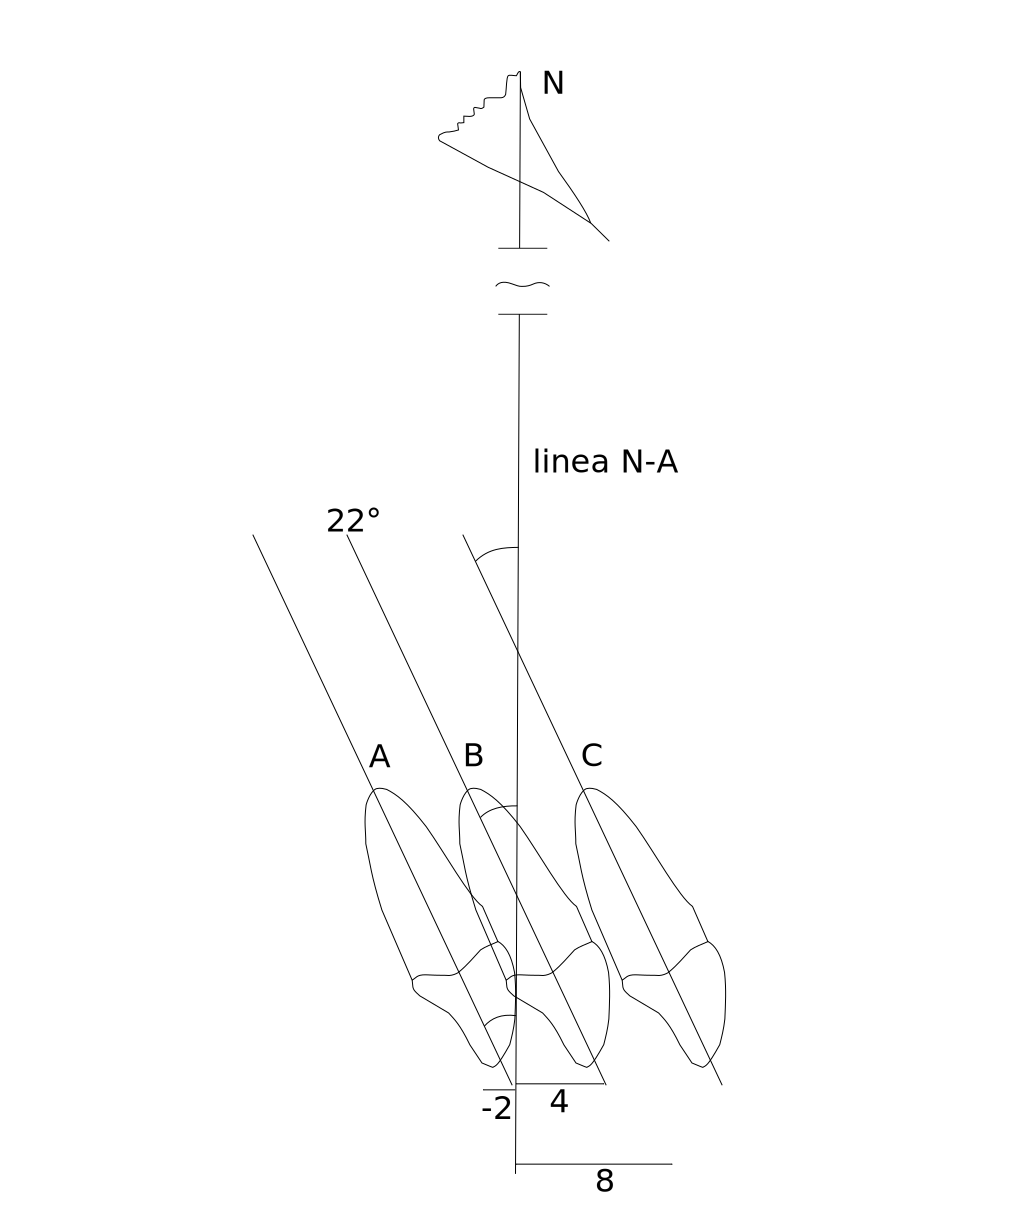
\includegraphics[width=.45\textwidth]{./images/steiner_incisivo_traslazione.pdf}}} \quad
\subfloat[][]
   {\label{fig:steiner_rotazione}\fbox{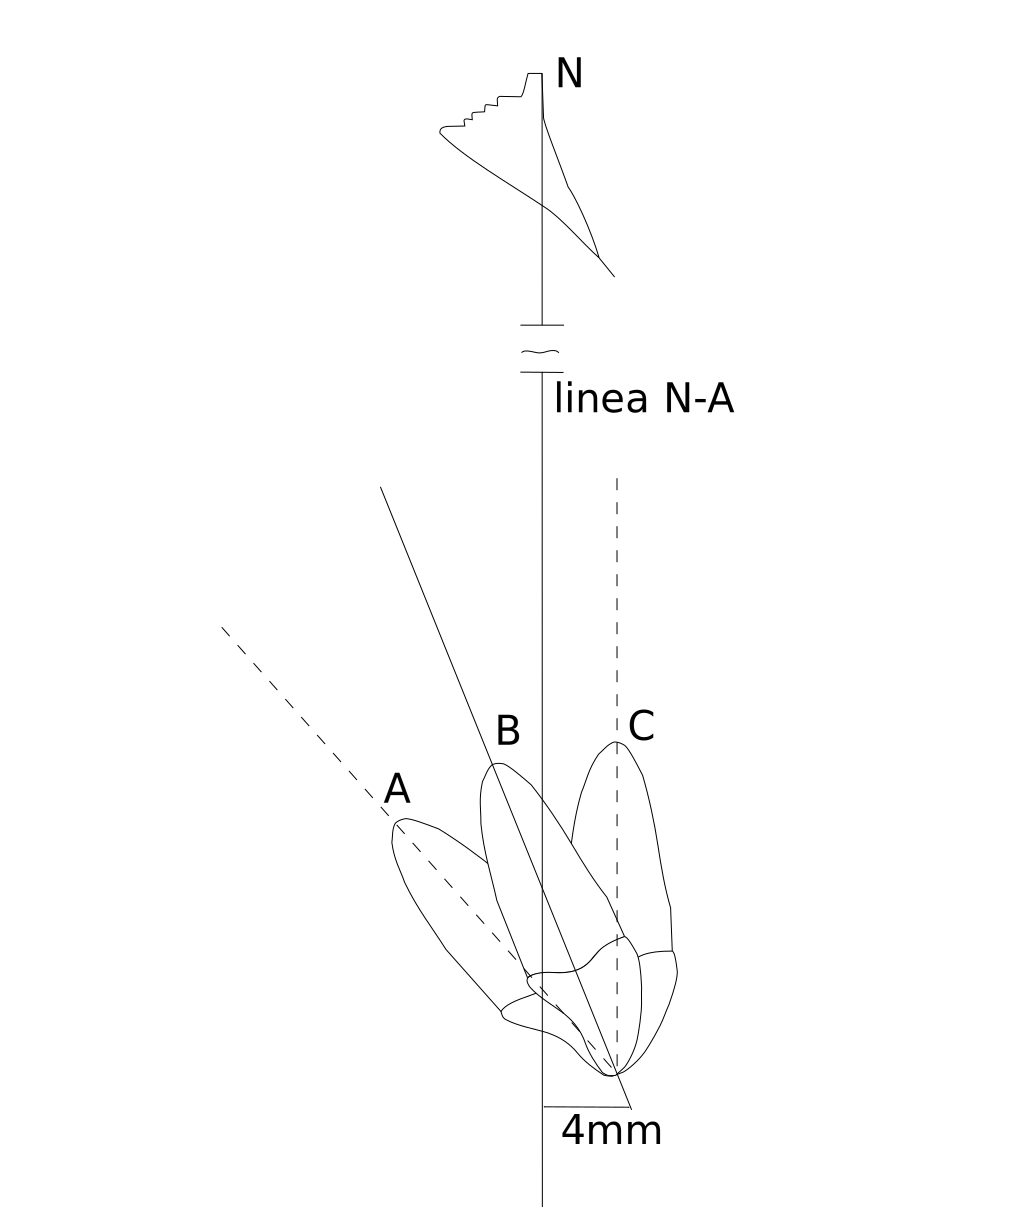
\includegraphics[width=.45\textwidth]{./images/steiner_incisivo_rotazione.pdf}}}
 \centering
 % steiner_sna.jpg: 1024x988 pixel, 72dpi, 36.12x34.85 cm, bb=0 0 1024 988
 \caption{Inclinazione e posizione dell'incisivo superiore, in relazione alla linea \punto{N}-\punto{A}: \subref{fig:steiner_traslazione} inclinazione corretta, ma posizione variabile; \subref{fig:steiner_rotazione} posizione corretta, ma inclinazione variabile.}
 \label{fig:steiner_incisivo_rototraslazione}
\end{figure}

\paragraph{Posizione incisivo inferiore}
Allo stesso modo che per l'incisivo superiore, per valutare la posizione dell'incisivo inferiore si misurano la distanza millimetrica tra superficie più labiale e linea \punto{N}-\punto{B}, e valore angolare tra questa e l'asse maggiore del dente. Anche in questo caso, Giannì propose la valutazione angolare rispetto al piano occlusale.

\begin{figure}[p!]
\centering
\begin{minipage}{.44\textwidth}
 \centering
 \fbox{
\includegraphics[width=.95\textwidth]{./images/steiner_interincisale.pdf}}
 \caption{Angolo interincisale}
 \label{fig:steiner_interincisale}
\end{minipage}\quad\quad
\begin{minipage}{.44\textwidth}
 \centering
 \fbox{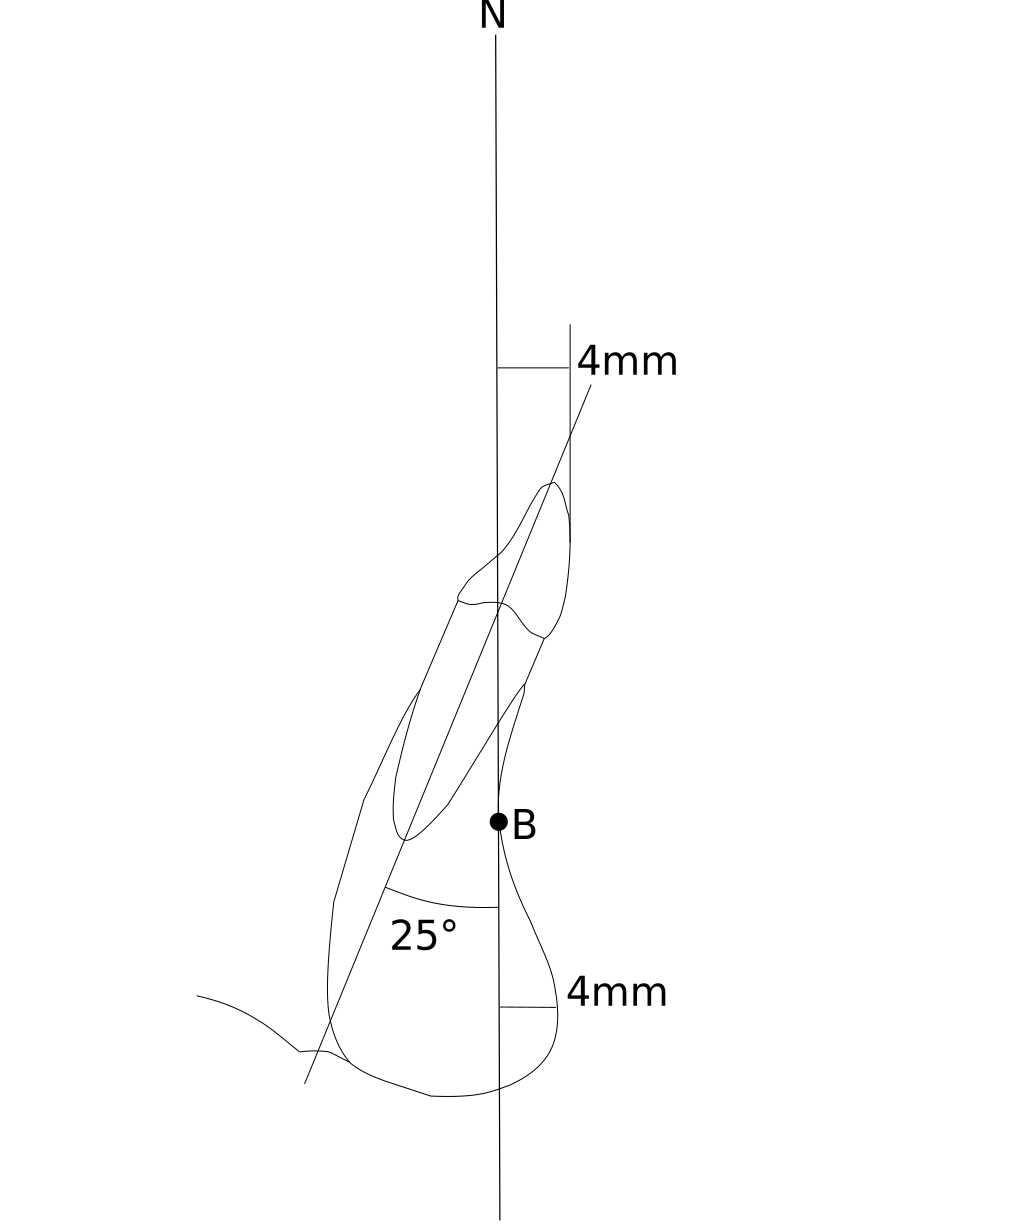
\includegraphics[width=.95\textwidth]{./images/steiner_incisivo_inferiore.pdf}}
 \caption{Rapporto tra incisivo inferiore, linea \punto{N}-\punto{B} e mento.}
 \label{fig:steiner_incisivo_inferiore}
\end{minipage}
\end{figure}

\paragraph{Angolo interincisale}
L'angolo interincisale (fig.~\vref{fig:steiner_interincisale}) mette in relazione la posizione degli incisivi centrali superiore e inferiore. Il valore medio è 130° $\pm$ 5°: valori minori o maggiori indicano una necessità di variazione dell'inclinazione di uno o entrambi gli incisivi. Nell'ipertono muscolare il valore angolare tende ad aumentare, e gli incisivi tendono alla palatinizzazione; viceversa nell'ipotono muscolare il valore angolare tende a diminuire, e gli incisivi tendono a vestibolarizzarsi.

\paragraph{Angolo occluso-molare superiore} introdotto da Giannì, obiettiva l'inclinazione del primo molare superiore rispetto al piano occlusale. Ha un valore medio di 90° $\pm$ 3°.

\paragraph{Posizione sagittale primo molare superiore} secondo Giannì. Viene valutata al fine di evidenziare la presenza di una mesializzazione dell'arcata dentaria superiore. Tale valutazione è basata sui rapporti tra il primo molare superiore e la retta \piano{S}{Gn}. Nella Classe I scheletrica, tale retta passa per il centro della cuspide mesio-vestibolare del primo molare superiore. La posizione del molare, però, dev'essere considerata in rapporto alla posizione delle basi ossee: è necessario quindi considerare anche l'angolo \angolo{ANB}. Per esempio, per un \angolo{ANB} di 5° (Classe II), è normale una mesializzazione del primo molare di 3mm: con la riduzione in Classe I (\angolo{ANB} di 2°), si avrà un avanzamento mandibolare di 3mm, per cui il molare sarà ben posizionato.

%\paragraph{Angolo bimolare inferiore} anch'esso introdotto da Giannì, è l'angolo formato tra l'asse maggiore del secondo molare inferiore e l'asse maggiore del terzo molare inferiore. La sua valutazione orienta sul tipo di eruzione del terzo molare inferiore. Un valore inferiore a 10° è indice favorevole all'eruzione e all'allineamento in arcata del terzo molare; con un valore superiore a 20° si ha, nella maggioranza dei casi, la disodontiasi del terzo molare.

\paragraph{Distanza tra \punto{N}-\punto{B} e il mento}
Visto il generoso contributo del mento al profilo facciale, è necessario tenerlo in considerazione nella valutazione cefalometrica. Il grado di prominenza del mento contribuisce al posizionamento dei denti in arcata. Idealmente, secondo Holdaway\footcite{Holdaway1956}, la distanza tra la linea \punto{N}-\punto{B} e il mento dovrebbe essere uguale alla distanza tra la stessa linea e la superficie più labiale dell'incisivo inferiore (fig.~\ref{fig:steiner_incisivo_inferiore}). Una discrepanza di 2mm tra questi valori è accettabile, 3mm è meno desiderabile, ma ancora tollerabile. Una discrepanza superiore ai 4mm, invece, richiede generalmente un intervento.

\section{Analisi dei tessuti molli}
L'analisi dei tessuti molli consiste in una registrazione grafica delle osservazioni cliniche effettuate durante l'esame del paziente. Essa include una valutazione dell'adattamento dei tessuti al profilo osseo sottostante, tenendo in considerazione dimensioni, forma e postura delle labbra. Viene inoltre analizzato lo spessore dei tessuti molli sulla sinfisi mentoniera e sulla struttura nasale, e al loro rapporto con la parte inferiore della faccia.

\begin{figure}[h!]
 \centering
 \fbox{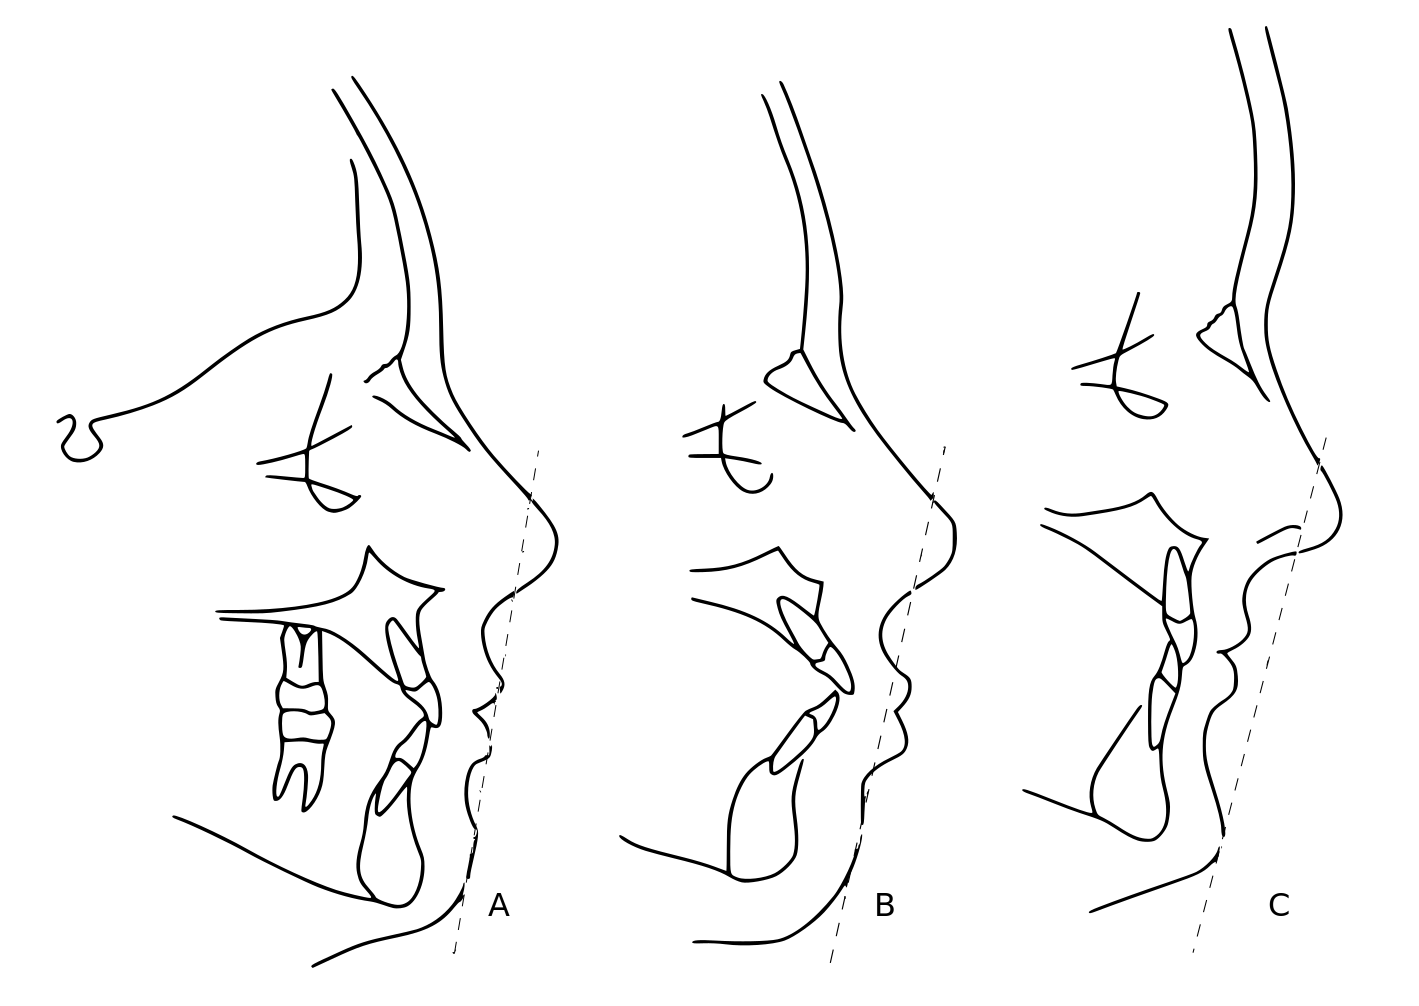
\includegraphics[width=.75\textwidth]{./images/steiner_linea_s.pdf}}
 % steiner_linea_s.jpg: 1419x1006 pixel, 72dpi, 50.06x35.49 cm, bb=0 0 1419 1006
 \caption{Linea S di Steiner: (a) labbra in equilibrio, (b) labbra protruse, (c) profilo retruso}
 \label{fig:steiner_linea_s}
\end{figure}

Steiner, Ricketts, Holdaway e Meddifield hanno sviluppato criteri e linee di riferimento per l'armonia del profilo facciale. Sebbene non possa esistere un concetto uniforme di cosa costituisca un profilo ideale, la \textit{linea S} di Steiner (fig.~\ref{fig:steiner_linea_s}) è molto usata nell'ortodonzia odierna per determinare l'equilibrio dei tessuti molli facciali. Le labbra, secondo Steiner, dovrebbero toccare una linea passante dal contorno del mento al punto mediano di una S formata dal bordo inferiore del naso. Questa linea viene chiamata \textit{linea S}.

Labbra posizionate oltre questa linea tendono alla protrusione, e il trattamento richiesto solitamente prevede un retroposizionamento dentale o scheletrico. Se invece le labbra sono posizionate posteriormente, il paziente ha un profilo generalmente interpretato come ``concavo'', la cui correzione ortodontica prevede un avanzamento dei denti, causando un avanzamento delle labbra.

Giannì effettua una modifica alla linea estetica di Steiner, tale da renderla attendibile nei casi di eccessivo o tardivo accrescimento della piramide nasale, secondo le critiche di Müller\footcite{Mueller1969}. Egli, infatti, considera come punto di mezzo del sotto-setto nasale (il ``centro'' della S secondo Steiner) il punto di mezzo di una linea perpendicolare alla retta \piano{N}{AN} (\punto{AN} è l'apice dell'osso nasale) passante per \punto{PS} (piede del sotto-setto nasale).

Nel caso in cui esistano le indicazioni clinica all'estrazione di premolari, la linea estetica è un'importante guida nella scelta dei premolari da estrarre. Se, infatti, il labbro dell'arcata coinvolta oltrepassa la linea estetica, allora è giustificata l'estrazione dei due primi premolari; è giustificata invece l'estrazione dei secondi premolari nel caso in cui il labbro coincida con la linea estetica. La spiegazione di questo ragionamento va ricercata nella stretta correlazione tra la zona delle estrazioni e il collasso del labbro: più le estrazioni sono posteriori, meno il labbro collassa e, pertanto, meno il profilo si modifica.

\chapter{Analisi di Ricketts}

Tutte le analisi cefalometriche prevedono l'identificazione di diversi punti craniofacciali. Molti di questi punti sono tradizionali; altri, invece, possono essere specifici di un'analisi in particolare. In questo capitolo si discuterà dell'analisi ideata da Robert M. Ricketts\footcite{Lucchese1988}.

\section{Punti cefalometrici}

\paragraph{Condilo (DC)} punto al centro del collo del condilo sul piano \piano{Na}{Ba}.

\paragraph{Centro del cranio (CC)} punto di intersezione del piano \piano{Na}{Ba} con l'asse facciale di Ricketts, che unisce \piano{PT}{Gn}.

\paragraph{CF} punto di intersezione del piano di Francoforte (\piano{Or}{Por}) con la verticale pterigoidea \punto{PTV}, retta perpendicolare al piano di Francoforte passante per il punto \punto{PT} e tangente il bordo posteriore della fessura pterigoidea.

\paragraph{Xi} punto geometrico del centro del ramo mandibolare. Per identificarlo, bisogna far riferimento al piano di Francoforte e al PTV, che sono tra loro perpendicolari. Localizzando la parte più interna della concavità anteriore del ramo della mandibola come R$_1$, si traccia da questo una retta parallela al piano di Francoforte, fino al bordo posteriore del ramo della mandibola R$_2$. Si definisce quindi R$_3$ come il punto più basso dell'incisura sigmoidea; facendo partire da questo una retta parallela a PTV, si ricava in basso il punto R$_4$. A questo punto si costruisce un rettangolo, tracciando parallele a PTV e al piano di Francoforte passanti per R$_1$, R$_2$, R$_3$ ed R$_4$. A questo punto si tracciano le diagonali del rettangolo, e il loro punto d'intersezione sarà il punto Xi.

\paragraph{Incision superiore (Is)} è il punto di contatto più basso degli angoli mesiali degli incisivi superiori, corrispondente alla parte più bassa del profilo del bordo incisivo superiore.

\paragraph{Incision inferiore (Ii)} è il punto di contatto più alto degli angoli mesiali degli incisivi inferiori, corrispondente alla parte più alta del profilo del bordo incisivo inferiore.

\paragraph{Pronasale cutaneo (Pn)} è il punto più sporgente della prominenza nasale.

\paragraph{Pogonion cutaneo (Po$_c$)} è il punto più sporgente dell'eminenza mentale.

\section{Analisi craniofacciale}

\begin{figure}[h!]
 \centering
 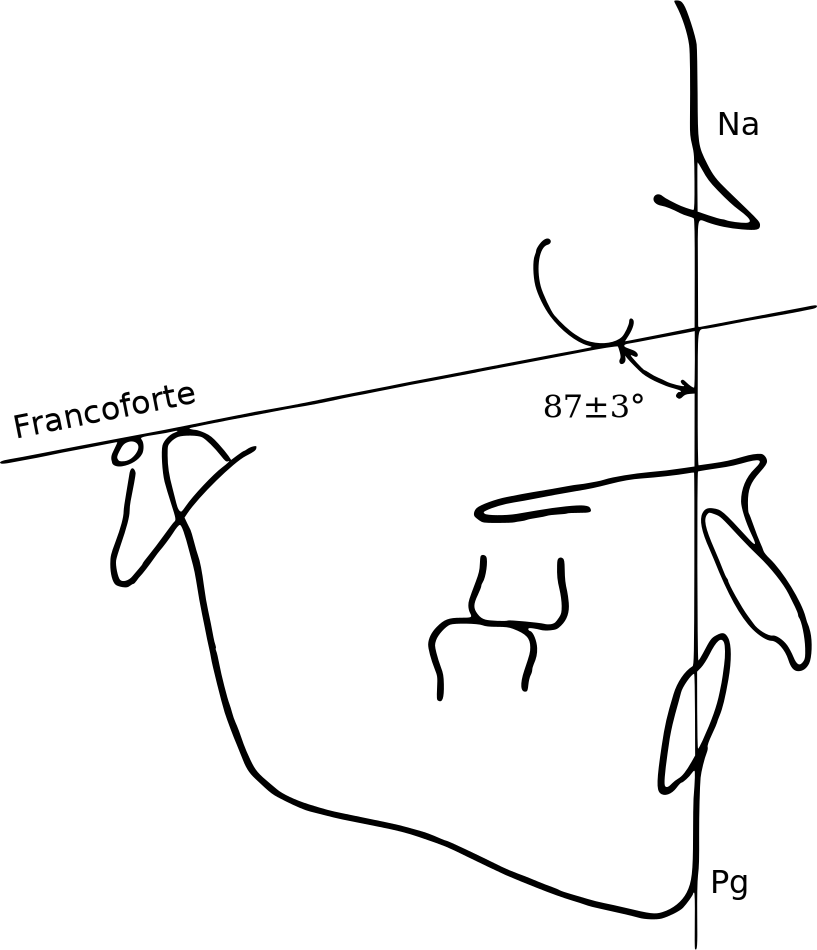
\includegraphics[width=.5\textwidth]{./images/ricketts_facciale_downs.pdf}
 % ricketts_facciale_downs.pdf: 654x760 pixel, 72dpi, 23.07x26.81 cm, bb=0 0 654 760
 \caption{Angolo facciale di Downs}
 \label{fig:ricketts_facciale_downs}
\end{figure}

\paragraph{Angolo facciale di Downs} (fig. \ref{fig:ricketts_facciale_downs}) dato dal piano facciale (\piano{Na}{Po}) col piano di Francoforte, indica la posizione più o meno avanzata della mandibola sul piano sagittale. Il valore medio è 87° a 9 anni, aumenta di 1° ogni 3 anni. La deviazione standard è $\pm$ 3°.

\paragraph{Asse facciale di Ricketts} linea che congiunge il punto \punto{PT} con lo Gnathion. Questa linea forma un angolo con il piano della base del cranio (\piano{Na}{Ba}) nella parte postero-inferiore il cui valore medio normale è di 90°, con una deviazione standard di $\pm$ 3°. Indica la traiettoria di crescita della mandibola: in avanti crescita orizzontale antioraria, in dietro e in basso crescita oraria, in avanti e in basso crescita neutrale; esprime la posizione della mandibola sul piano verticale.

\paragraph{Angolo della conicità facciale} o angolo piano facciale-piano mandibolare: indicativo dello sviluppo in altezza della parte posteriore della faccia. Ha un valore medio di 68°, con una deviazione standard di $\pm$ 4°. Un angolo superiore indica un soggetto ortognatico (brachi-facciale), un angolo inferiore un soggetto prognatico (dolico-facciale).

\paragraph{Angolo piano di Francoforte-piano mandibolare} esprime il grado di inclinazione mandibolare, e la posizione verticale della mandibola. Ha un valore medio di 26°, che diminuisce con l'età, con una deviazione standard di $\pm$ 4°. Un angolo superiore indica un soggetto prognatico (dolico-facciale), un valore inferiore un soggetto ortognatico (brachi-facciale).

\paragraph{Angolo piano di Francoforte-piano \piano{Na}{A}} è la profondità mascellare, indica la posizione più o meno avanzata del mascellare superiore sul piano sagittale. Ha un valore medio di 90° $\pm$ 3°.

\paragraph{Angolo piano \piano{Na}{CF} con il piano \piano{CF}{A}} è l'altezza mascellare superiore, indica la posizione del mascellare superiore sul piano verticale. Ha un valore medio di 54°, che aumenta di 1° ogni 3 anni. La deviazione standard è $\pm$ 3°.

\paragraph{Angolo piano di Francoforte con il piano bispinale} è indicativo dell'orientamento del mascellare superiore verso l'alto o verso il basso. Ha un valore medio di 1° $\pm$ 3°.

\paragraph{Angolo \piano{Na}{Ba} con il piano di Francoforte} angolo supero-anteriore, esprime il grado di inclinazione della base cranica. Ha un valore medio di 26° $\pm$ 2°. Valori superiori indicano una crescita verso il basso del Basion (crescita antioraria); valori inferiori indicano una crescita in dietro del Basion (crescita oraria).

\paragraph{Lunghezza base cranica anteriore} misurata tra il punto \punto{CC} e il punto \punto{Na}. Ha un valore medio di 56 $\pm$ 3mm a 10 anni, e aumenta di $0,8$ mm ogni anno. Valori superiori indicano che il soggetto è di tipo prognatico (dolico-facciale), valori inferiori che il soggetto è ortognatico (brachi-facciale).

\paragraph{Altezza facciale posteriore} distanza \punto{CF}-\punto{Go}, ha un valore medio di 56 $\pm$ 4mm. Valori superiore indicano un aumento in altezza del ramo mandibolare, valori inferiori ne indicano un accorciamento.

\paragraph{Posizione del Porion} distanza tra il Porion e il piano pterigoideo verticale. Valore medio di 39 $\pm$ 2mm, aumenta di $0,5$mm per anno.\footnote{FIXME: a che età è la media?}

\paragraph{Angolo piano \piano{CF}{Xi} con la linea verticale pterigoidea} dà la posizione del ramo mandibolare, ha un valore medio di 15 $\pm$ 3°. Valori superiori indicano una crescita posteriore della mandibola, valori inferiori una crescita anteriore.

\paragraph{Angolo dell'arco mandibolare} formato dal prolungamento dell'asse del corpo mandibolare con l'asse condilare. Il valore medio è di 27 $\pm$ 5° a 9 anni; valori superiori indicano che la mandibola è orientata orizzontalmente, mentre valori inferiori indicano che la mandibola è orientata in basso e indietro, cioè il corpo mandibolare è molto inclinato.

\paragraph{Lunghezza del corpo mandibolare} è data dalla distanza \punto{Pm}-\punto{Xi}. Il valore medio è di 66mm a 9 anni, con un range di variazione dai 64 ai 70mm. Indica il grado di sviluppo mandibolare: valori inferiori indicano che la mandibola è corta, valori superiori indicano una mandibola lunga.

\section{Analisi del sistema scheletrico}
\paragraph{Convessità} è data dalla distanza del punto \punto{A} dal piano facciale. Valori medi normali sono da 3 a 5mm, con una deviazione standard di $\pm$ 2mm. La convessità è indicativa della posizione del mascellare superiore in rapporto alla mandibola. Essa è positiva quando il punto \punto{A} è anteriore al piano facciale, e indica un modello scheletrico di Classe II. È invece negativa quando il punto \punto{A} è posteriore al suddetto piano, e indica un modello scheletrico di Classe III. La convessità diminuisce con l'età, soprattutto in pazienti con un buon potenziale di crescita orizzontale.

\paragraph{Altezza facciale inferiore} è data dal valore dell'angolo \punto{SNA}-\punto{Xi}-\punto{Pm}, il cui valore medio normale è di 47 $\pm$ 4°. Quest'angolo non si modifica con la crescita.

\section{Analisi dentale}

\paragraph{Relazione dei molari sul piano sagittale} viene calcolata la distanza tra le superfici distali dei primi molari superiori ed inferiori, misurati sul piano occlusale. Valori medi sono:
\begin{itemize}
\item Classe I: -3mm;
\item Classe II: 0mm o maggiore;
\item Classe III: -6mm.
\end{itemize}

Valori negativi sono indicativi di una posizione distale dei molari superiori rispetto agli inferiori.

\paragraph{Relazione dei canini sul piano sagittale} è data dalla distanza tra le cuspidi dei canini misurata sul piano occlusale.
\begin{itemize}
\item Classe I: -2 $\pm$ $0,7$mm;
\item Classe II: +1mm;
\item Classe III: -5 $\pm$ 3mm.
\end{itemize}

\paragraph{Rapporto tra incisivi superiori ed inferiori sul piano antero-posteriore (\textit{overjet})} distanza sagittale dei margini incisivi misurata sul piano occlusale. Valore medio $2,5$ $\pm$ $2,5$mm.

\paragraph{Rapporto verticale tra incisivi superiori ed inferiori (\textit{overbite})} distanza verticale tra i margini incisivi, misurata perpendicolarmente al piano occlusale. Valore medio $2,5$ $\pm$ 2mm.

\paragraph{Angolo interincisivo}, formato dagli assi degli incisivi. Valore medio 130 $\pm$ 6°. Per i soggetti prognatici il valore normale varia da 115° a 125°, per i soggetti ortognatici da 135° a 145°.

\section{Rapporti dento-scheletrici}

\paragraph{Posizione del primo molare superiore} data dalla distanza tra la superficie distale del sesto superiore e il piano pterigoideo verticale. Il valore medio normale è uguale all'età del paziente $+$ 3 $\pm$ 3mm.

\paragraph{Posizione dell'incisivo inferiore in relazione ai mascellari} data dalla distanza del margine incisale inferiore dalla linea \piano{A}{Po}, con un valore medio di $2,4$ $\pm$ 2mm. La misura è positiva quando l'incisivo è davanti alla linea \piano{A}{Po}, negativa quando è indietro.

\paragraph{Inclinazione dell'incisivo inferiore} misurata dall'angolo che l'asse incisivo inferiore forma con la linea \piano{A}{Po}. Ha un valore medio di 22 $\pm$ 4°; valori superiori indicano un tipo scheletrico prognatico (dolico-facciale), valori inferiori un tipo ortognatico (brachi-facciale).

\paragraph{Inclinazione dell'incisivo superiore} misurata dall'angolo che l'asse incisivo superiore forma con la linea \piano{A}{Po}. Ha un valore medio di 28 $\pm$ 4°, e dev'essere parallelo all'asse facciale.

\paragraph{Inclinazione del piano occlusale} è data dall'angolo che il piano occlusale forma con l'asse del corpo mandibolare. Ha un valore medio di 22° a 8 anni e 20° a 12 anni, e diminuisce di $0,5$° ogni anno. Ha una deviazione standard di $\pm$ 2°.

\section{Analisi estetica}

\paragraph{Rapporto del labbro inferiore con la linea estetica E di Ricketts} il cui valore medio è $-$2 $\pm$ 2mm. Con il labbro in posizione normale va da $-$2 a 0mm. Il labbro si dice retruso se è oltre i $-$3mm, altrimenti è protruso oltre i 3mm.

\part*{Analisi proporzionali}
\chapter{Analisi delle controparti di Enlow}
Quest'analisi rappresenta il metodo cefalometrico secondo Donald Enlow, in cui le varie parti facciali e craniche vengono paragonate le une alle altre: il soggetto in esame viene confrontato con sé stesso, e non con la media della popolazione.\\

Prima di descrivere il metodo dettagliatamente è necessario soffermarsi su due termini: \emph{dimensione} (orizzontale e verticale) e \emph{allineamento} (tipo di rotazione) dell'osso.

La \emph{dimensione} rappresenta la misura assoluta di una lunghezza; una determinata zona può essere lunga o corta rispetto al suo combaciamento con le altre parti vicine.

L'\emph{allineamento} rappresenta la misura relativa di una lunghezza che, proiettata su un piano di riferimento, ha subito una rotazione; qualsiasi movimento di rotazione infatti può aumentare o diminuire la misura della proiezione di una dimensione.

Pertanto, per poter analizzare tra loro due controparti non è sufficiente conoscerne la dimensione, ma è necessario anche valutarne l'allineamento e comprendere quanto questo influisca sulle loro effettive dimensioni.

Il principio razionale di questa analisi è il confronto tra la dimensione verticale e/o la dimensione orizzontale di una parte con la sua controparte specifica. Se esse corrispondono, esiste un equilibrio dimensionale; al contrario se divergono, lo squilibrio che ne risulta pu causare un effetto di retrusione o di protrusione della parte coinvolta.\\

Nell'analisi delle controparti di Enlow sono previste due fasi:
\begin{enumerate}
\item una \emph{statica}, in cui ogni parte è paragonata alla sua controparte senza considerare le medie della popolazione (tracciato funzionale);
\item una \emph{dinamica}, in cui il soggetto viene confrontato con un tracciato ideale.
\end{enumerate}

\section{Punti di repere}
\section{Linee, piani ed angoli della base cranica}
\section{Linee, piani ed angoli della base cranica nel tracciato neutro}
\section{Analisi statica del tracciato cefalometrico}
\subsection{Analisi dell'equilibrio verticale}
\subsection{Analisi dell'equilibrio orizzontale}
\section{Analisi dinamica del tracciato cefalometrico}
\section{Casi clinici}
\chapter{Analisi proporzionale di Coben}
\section{Casi clinici}

\chapter{Analisi architetturale di Delaire}
\nocite{Delaire1981,Cudia1991}

L'analisi cefalometrica proposta da Delaire è un'analisi architettonica e strutturale che considera linee verticali e orizontali tracciate a partire da punti di repere anatomici non convenzionali.\\
Per poter utilizzare tale analisi sarà necessario avere una buona teleradiografia, perché il tracciato prende in esame le strutture cranio-maxillo-rachidee.\\

Si distinguono le strutture craniche da quelle mascellari, le prime individuate dalle sigle da C1 a C4, le seconde da CF1 a CF8, rispettivamente \emph{linee craniche} e \emph{linee cranio-facciali}.\\

\section{Linee craniche}
\paragraph{C1} suddivide la parte cranica da quella maxillo-rachidea, e ne indica la sua lunghezza. Viene tracciata fino ad un punto \punto{OI} (occipitale inferiore), dal quale si traccia la tangente alla parte prominente dell'occipite.\\
C1 si traccia a partire dal punto \punto{M}, punto di unione delle ossa naso-fronto-mascellare sulla parte inferiore della sutura stessa e passante per il punto di incontro tra il condilo zigomatico e quello temporale, punto \punto{CT}.

\paragraph{C2} indica la lunghezza della volta cranica nella proporzione 80-85\% della lunghezza di \punto{C1}. Si traccia perpendicolarmente a partire dal punto di mezzo di C1; nella norma dovrebbe cadere dietro il condilo, punto \punto{CP}, cioè separare la parte rachidea dalla parte maxillo-mandibolare.\\
La parte mandibolare è a sua volta il 40\% e la mascellare il 60\% del tratto \piano{M}{CP}, sempre considerando la norma. Se C2 non è tangente al bordo posteriore del condilo si può fare subito una considerazione sul mancato equilibrio della parte rachidea e maxillo-mandibolare a favore della parte rachidea, per esempio nelle terze classi a crescita verticale o di quella mascellare nei casi di terza classe a crescita orizzontale, nelle retrognazie e nei deep-bite. Così pure la proporzione 40-60\% tra i mascellari può variare ed esprimere squilibri tra le due parti, per esempio una proporzione maggiore a favore del mascellare nelle prognazie superiori.

\paragraph{C3} tracciata dal punto \punto{M}, passa per i processi clinoidei posteriori fino all'occipite. È la linea della base cranica, piano di riferimento delle strutture sottostanti.

\paragraph{C4} o \emph{linea del clivus}, va dalla metà dei processi clinoidei posteriori al bordo postero-superiore del dente dell'epistrofeo. C4 definisce insieme a C3 l'angolo posteriore della base cranica. Il valore si aggira intorno a 114° nelle femmine e 112° nei maschi per l'angolo posteriore, mentre l'angolo anteriore definito tra C3 a C1 è di circa 22°.

\section{Strutture mascellari}
\paragraph{Pilastro anteriore} è la struttura più importante da individuare, tracciare e considerare in tutto il tracciato. Esso corrisponde ad una struttura anatomica ben definita dall'addensamento trabecolare di rinforzo in corrispondenza della branca anteriore del mascellare. Si tratta di una struttura paramediana ma unica nelle teleradiografie latero-laterali.\\

Il pilastro anteriore è espresso dalla linea \punto{CF1} tracciata da \punto{Fm}, cioè un millimetro e mezzo dietro \punto{M} in corrispondenza della perpendicolare a \punto{C3}, tracciata dalla cresta di rinforzo sul fondo del seno frontale (talvolta sono individuabili due creste e la perpendicolare a C3 si traccia a partire dal punto di mezzo tra queste).\\

Lungo il suo percorso, la linea CF1 incontra il punto orbitale inferiore e il canale palatino anteriore, corrispondente quasi sempre all'apice del canino permanente o all'hipomoclion del canino in formazione. XXX FIXME XXX

Questi tre punti, soprattutto nelle terze classi, non sono ben allineati e il pilastro anteriore si fa passare per il punto \punto{Fm} e \punto{orbitale inferiore}. Il pilastro anteriore è quello che subisce maggiori alterazioni nelle varie patologie seguendo le alterazioni del mascellare superiore, che può avere un aggetto verso l'esterno normale, aumentato o diminuito. Esistono dunque due pilastri anteriori: quello \emph{reale}, dato dalle strutture che si considerano sulla teleradiografia, e quello \emph{ideale}, che considera lo sviluppo che il mascellare dovrebbe avere se tutte le strutture fossero nella norma. Dal confronto si ha la conoscenza della deviazione nella patologia considerata.\\

Il calcolo dell'aggetto del pilastro anteriore ideale prende in considerazione il fatto che la sua crescita in avanti aumenta con l'età e il suo valore angolare, calcolato tra \punto{C1} e \punto{CF1}, va da 80° nei bambini più piccoli a 90° negli adulti, con valori leggermente inferiori nelle donne. L'angolo ideale sarà tracciato considerando l'età del paziente, o anche aggiungendo al valore dell'angolo della base anteriore del cranio il valore di 65. Inoltre il pilastro ideale è tangente all'apice dell'incisivo inferiore, e taglia la sinfisi tra il terzo medio e quello posteriore.\\

Il primo dato diagnostico ci è riferito dal \emph{confronto tra pilastro reale e ideale}; il secondo, più importante, è dato dal \emph{punto di tangenza del pilastro ideale e la sinfisi}. Se cade sul bordo posteriore della sinfisi si può dire che la mandibola è grande; se cade davanti, che è piccola. Questi valori non devono però essere solo correlati tra loro, ma devono essere valutati altri dati -- per esempio, la rotazione della mandibola -- perché in caso di rotazione posteriore, una mandibola più grande della norma può esere tagliata da CF1 tra terzo medio e terzo posteriore della sinfisi o nella sua parte anteriore.\\

Altra situazione da considerare, sempre in relazione a CF1, è una mandibola piccola ma mesializzata, che si troverà in posizione di normalità rispetto a CF1. Questo dato sarà controllato dalla posizione del bordo posteriore della mandibola rispetto al bordo anteriore del tratto cervicale.

\paragraph{Pilastro medio} o \punto{CF2}, è il segmento che congiunge il \punto{bregma} al punto \punto{Pts}. Pts è il punto di mezzo del tratto postero-superiore della fessura pterigo-mascellare che si ottiene tracciando la bisettrice dell'angolo formato da \punto{C1} e la retta tangente al processo pterigoideo dello sfenoide.\\
La parte terminale di \punto{CF2} divide la mandibola in due parti uguali. Se le due parti non sono uguali ci si può trovare in presenza di una mandibola piccola o distalizzata (parte anteriore diminuita o postruotata). Se la parte posteriore è più piccola, la mandibola può essere in protrusione oppure aumentata di volume.\\

\paragraph{Pilastro posteriore} o \punto{CF3}, si traccia parallelamente a \punto{CF2} perché così è orientato nelle strutture normali, partendo dal punto di tangenza di \punto{C1} con il condilo, cioè il punto \punto{Cp}.

Anche in questo caso si tracciano due pilastri posteriori, uno ideale, parallelo, e uno reale, tangente al bordo posteriore della mandibola, sempre partendo dal punto \punto{Cp}. Nei casi di normalità di posizione mandibolare i due coincidono, nel caso contrario possono indicare una mandibola retrusa o protrusa, eccessi di sviluppo della zona dell'angolo mandibolare o un'eccessiva inclinazione della branca montante con apertura dell'angolo.

\paragraph{Piano bispinale} o \punto{CF4}. Nella norma, la spina nasale posteriore e quella anteriore sono allineate con l'articolazione occipito-rachidea, il dente dell'epistrofeo e l'arco dell'atlante.\\

In un'età vicina alla pubertà il dente dell'epistrofeo e l'arco dell'atlante sono tagliati nella loro parte superiore, ma in un bambino di giovane età si trovano al di sotto della congiungente i condili occipitali e la linea bispinale. La ragione risiede nel fatto che nel processo di crescita le vertebre cervicali si sviluppano più verso l'alto che il basso. Questi punti possono quindi coincidere o meno. Quando nessun punto coincide con l'articolazione occipito-rachidea si devono tracciare diverse linee passanti per i diversi punti, cioè si costituisce una \emph{banda} e la linea di mezzo sarà quella alla quale ci si riferisce.\\
\\
Da CF4 risulta evidente la posizione della spina nasale anteriore, che può trovarsi verso l'alto, come nei morsi aperti, o verso il basso, nei morsi chiusi. La stessa sorte può subire la spina nasale posteriore che, a seconda dei movimenti della lingua, può orientarsi verso l'alto o verso il basso.

\paragraph{Altezza facciale} espressa da \punto{CF5}, è tracciata a partire dal punto SNA, reale se si colloca sul piano bispinale, oppure ideale se si trova sul CF4 ricavato dalla banda di linee di cui sopra. Da questo punto si traccia una perpendicolare fino al punto \punto{N}, o meglio \punto{Na'}, perché la retta giace al di fuori del cranio e, nei casi di ipomaxillia grave, talvolta all'interno.\\

\punto{CF5}, misurato come \piano{Na'}{Met'}, viene calcolato raddoppiando la distanza \piano{SNA}{Na'} e aggiungendo un nono della misura trovata. Il punto trovato è \punto{Met'}, e viene riportato sul pilastro ideale, tracciando una perpendicolare da \punto{Met'} al pilastro stesso, e viene indicato con \punto{Met}.\\

\paragraph{Piano mandibolare} \punto{CF6}, indica il piano mandibolare tracciato da \punto{Met} e tangente alla squama dell'occipitale. Incontra \punto{CF4} in un punto \punto{OM}. Questa linea indica lo sviluppo del bordo inferiore della mandibola, il grado dello sviluppo del ramo perlopiù diminuito nelle iperdivergenze, lungo per esempio in certe sindromi come l'acromegalia e in certi casi di \emph{long face} a ramo lungo. Evidenzierà anche il grado di post-rotazione mandibolare, il cui bordo eccederà dal piano mandibolare stesso.

\paragraph{Piano occlusale} espresso da \punto{CF7}, si presenta anch'esso in due modalità, una reale e una ideale. Il piano occlusale reale corrisponde al piano occlusale di Ricketts, mentre quello ideale corrisponde alla metà della distanza tra \piano{SNA}{Met'}, che si congiunge indietro nel punto \punto{OM}.\\

\paragraph{CF8} è l'ultimo piano da considerare, tracciato parallelo a \punto{C3} a partire da \punto{SNA}, reale o ideale, fino a raggiungere la zona dell'angolo che potrà coincidere o no col vertice dell'angolo. Dà utili indicazioni sull'angolo e sulla lunghezza del ramo della mandibola e la lunghezza di questo in relazione a quella della branca montante del mascellare. Nella norma, il ramo mandibolare è più lungo del mascellare.

%La ricchezza degli elementi considerati, e soprattutto il fatto che gli elementi scheletrici siano cranio-maxillo-rachidei, permette una grande elaborazione di dati: correlando gli uni agli altri si può, per via induttiva e deduttiva, porre le basi per una buona diagnosi.

\chapter{Analisi di Sassouni}
L'analisi di Sassouni (1955, 1969) è una \textit{analisi archiale}, una delle prime a considerare il complesso dentofacciale come un'unica unità all'interno del pattern individuale\footnote{figura?}.

L'analisi di Sassouni, detta da alcuni autori la \textit{rosa dei venti}, si basa sul disegno di quattro archi, con centro O (definito come il punto di convergenza della parallalela alla linea sopraorbitale, del piano palatale, del piano occlusale e del piano mandibolare):

\begin{description}
\item[arco anteriore] passante per N;
\item[arco basale] passante per A;
\item[arco mediofacciale] passante per Te;
\item[arco posteriore] passante per Sp.
\end{description}

Quest'analisi prevede una \textit{valutazione visiva} delle tendenze indicative di una faccia ben proporzionata:

\begin{enumerate}
\item convergenza delle linee parallele al margine sopraorbitale;
\item convergenza dei piani palatale, occlusale e mandibolare verso il punto O;
\item l'arco anteriore dovrebbe passare per SNA, il margine incisale dell'incisivo superiore e Pog;
\item l'arco basale dovrebbe passare per il punto B;
\item l'arco mediofacciale, indicativo della posizione dei primi molari, dovrebbe passare tangente alla superficie mesiale del primo molare superiore, quando l'arco anteriore passa per SNA;
\item l'arco posteriore, indicativo della posizione posteriore della mandibola, dovrebbe passare da Go.
\end{enumerate}

Verticalmente, l'altezza facciale superiore e quella inferiore dovrebbero coincidere, sia anteriormente che posteriormente. La lunghezza Go-Pog dovrebbe essere pari alla base cranica (Sp-N, lungo il raggio), estendendosi tra l'arco anteriore e quello posteriore. L'angolo tra il piano della base cranica e il piano palatale dovrebbe essere uguale all'angolo palatomandibolare.

Quest'analisi fornisce un metodo analitico rapido, semplice e conveniente, sebbene localizzare il punto O possa essere talvolta difficile.

\begin{table}[h]
\footnotesize
\caption{Punti e piani specifici dell'analisi di Sassouni}
\begin{tabularx}{\textwidth}{>{\textit}clX}
\toprule
\multicolumn{3}{l}{\textbf{Punti di repere}} \\
\midrule
O & Punto O & L'intersezione o il punto di convergenza della parallela al piano sopraorbitale, il piano palatale, il piano occlusale e il piano mandibolare.\\
Si & Pavimento della sella & Il punto più basso del contorno della sella turcica. \\
Sp & Dorso della sella & Il punto più posteriore sul profilo della sella turcica. \\
Te & Temporale & L'intersezione della lamina cribrosa dell'etmoide e la parete anteriore della fossa infratemporale con il punto superiore del tetto dell'orbita. \\
\midrule
\multicolumn{3}{l}{\textbf{Piani}} \\
\midrule
Me-Go & Mention-Gonion & Rappresenta l'estensione della base mandibolare. \\
Ar-Go & Piano del ramo & Rappresenta la lunghezza del ramo mandibolare. \\
Te-ClinAnt & Piano sopraorbitale & Linea tangente a Te e al processo clinoideo anteriore dello sfenoide. \\
 & Parallela al piano sopraorbitale & Linea tangente a Si parallela al piano sopraorbitale. \\
Or-ClinAnt & Piano infraorbitale & Linea tangente ad Or e al processo clinoideo anteriore dello sfenoide. \\
 & Piano ottico & Costruito disegnando la bisettrice dell'angolo formato dai piani sopra e infraorbitale. \\
 & Lunghezza mascellare & Distanza lineare (\textit{mm}) da SNA a SNP. \\
 & Lunghezza mandibolare & Distanza lineare (\textit{mm}) da Go a Pog. \\
\bottomrule
\end{tabularx}
\end{table}

\section{Casi clinici}

\chapter{Discussione}
Questo studio prevede la valutazione di alcuni parametri utilizzando diverse tecniche cefalometriche, e analizzati in senso statistico.
%Verranno di seguito analizzati i risultati delle misurazioni effettuate su due piani:  antero-posteriore (classe scheletrica) e verticale (rotazione del piano occlusale).

\section{Classe scheletrica}
Per valutare il rapporto antero-posteriore tra il mascellare superiore e la mandibola (\emph{classe scheletrica}) sono state prese in considerazione cinque analisi cefalometriche: tre riferite a valori statistici (Giannì, Wits, Ricketts), e due riferite a valori proporzionali (Enlow, Coben).

Per quanto riguarda l'analisi di Giannì, è stato valutato l'angolo \angolo{ANB}; l'indice di Wits è notoriamente la distanza millimetrica \piano{$A_0$}{$B_0$} sul piano occlusale; in Ricketts viene valutato l'angolo facciale (\piano{N}{Pog} su \punto{FH}) e la convessità facciale (distanza ortogonale di \punto{A} da \piano{N}{Pog}). Nell'analisi delle controparti di Enlow è stata valutata la discrepanza tra le controparti mascellare basale (\piano{A}{PM}) e mandibolare basale (\piano{B$\perp$REF}{ARA}). In Coben sono state fatte due valutazioni, differenti tra loro nel riferimento mandibolare: \piano{Ba}{Pog} per una, e \piano{Ba}{B} per l'altra, entrambe rapportate a \piano{Ba}{A}. Queste verranno in seguito denominate ``Coben \punto{Pog}'' e ``Coben \punto{B}'', rispettivamente.

Dato che non esiste un \emph{gold standard} per il rilevamento della classe scheletrica, sono stati eseguiti tre \emph{test $\chi^2$ di Pearson}, considerando \emph{standard} di volta in volta le tre analisi riferite a valori statistici. L'ipotesi nulla ($H_0$) è, in tutti e tre i casi, che \emph{non esiste alcuna differenza tra le analisi considerate}.

La tabella delle frequenze delle classi scheletriche (\ref{tab:classe_scheletrica_frequenze}) mostra già un'evidente discordanza numerica nel rilevamento delle III classi tra Giannì e le altre analisi.

\begin{table}
\centering
\caption{Frequenza delle classi scheletriche}
\label{tab:classe_scheletrica_frequenze}
\begin{tabular}{>{\bfseries}c*{6}{c}}
\toprule
Classe & Enlow & Giannì & Wits & Ricketts & Coben \punto{Pog} & Coben \punto{B} \\
\midrule
I & 11 & 16 & 13 & 18 & 11 & 9 \\
II & 11 & 12 & 8 & 8 & 12 & 13 \\
III & 7 & 1 & 8 & 3 & 6 & 7 \\
\bottomrule
\end{tabular}
\end{table}

Calcolando il $\chi^2$ con grado di libertà 2, e il valore $p$ (vedi paragrafo \ref{sec:chi-square} a pagina \pageref{sec:chi-square}) si ottengono le tabelle \ref{tab:classe_scheletrica_chi-quadro} e \ref{tab:classe_scheletrica_p-value} (in evidenza i valori di $p$ statisticamente significativi).

\begin{table}
\centering
\caption{Test del $\chi^2$ sulle classi scheletriche}
\label{tab:classe_scheletrica_chi-quadro}
\begin{tabular}{>{\bfseries}c*{6}{D{,}{,}{2.2}}}
\toprule
 & \multicolumn{1}{c}{Enlow} & \multicolumn{1}{c}{Giannì} & \multicolumn{1}{c}{Wits} & \multicolumn{1}{c}{Ricketts} & \multicolumn{1}{c}{Coben \punto{Pog}} & \multicolumn{1}{c}{Coben \punto{B}} \\
\midrule
Giannì & 37,65 & 0 & 50,90 & 5,58 & 26,56 & 39,15 \\
Wits & 1,56 & 8,82 & 0 & 5,05 & 2,81 & 4,48 \\
Ricketts & 9,18 & 3,56 & 9,72 & 0 & 7,72 & 12,96 \\
\bottomrule
\end{tabular}
\end{table}

\begin{table}
\centering
\caption{Valori $p$ nei test del $\chi^2$ sulle classi scheletriche}
\label{tab:classe_scheletrica_p-value}
\begin{tabular}{>{\bfseries}c*{6}{c}}
\toprule
 & \multicolumn{1}{c}{Enlow} & \multicolumn{1}{c}{Giannì} & \multicolumn{1}{c}{Wits} & \multicolumn{1}{c}{Ricketts} & \multicolumn{1}{c}{Coben \punto{Pog}} & \multicolumn{1}{c}{Coben \punto{B}} \\
\midrule
Giannì & \cellcolor[gray]{.8} $< 0,0001$ & $1$ & \cellcolor[gray]{.8} $< 0,0001$ & $0,0613$ & \cellcolor[gray]{.8} $< 0,0001$ & \cellcolor[gray]{.8} $< 0,0001$ \\
Wits & $0,4589$ & \cellcolor[gray]{.8} $0,0122$ & $1$ & $0,0801$ & $0,2457$ & $0,1064$ \\
Ricketts & \cellcolor[gray]{.8} $0,0101$ & $0,1690$ & \cellcolor[gray]{.8} $0,0077$ & $1$ & \cellcolor[gray]{.8} $0,0210$ & \cellcolor[gray]{.8} $0,0015$ \\
\bottomrule
\end{tabular}
\end{table}

Questi dati mettono in evidenza come, considerando \emph{standard} le analisi di Giannì e Ricketts, si ottengano valori $p$ statisticamente significativi quando paragonate con le analisi di Enlow, Wits e Coben. Questo significa che l'\emph{ipotesi nulla} è rigettata per queste tre analisi, ossia le differenze tra le diagnosi effettuate sono \emph{statisticamente significative}. Sembrerebbe che, invece, considerando come standard l'indice di Wits, le differenze siano meno significative, eccezion fatta per l'analisi di Giannì.


\section{Altezza facciale inferiore}

\section{Rotazione del piano occlusale}
Per poter valutare la rotazione del piano occlusale è necessario considerare che l'analisi delle controparti di Enlow non fornisce dei valori di riferimento, per cui bisogna valutare il rapporto delle controparti verticali tra di loro. Per far questo, verrà utilizzato lo \emph{scostamento medio} descritto nel paragrafo \vref{scostamento_medio}. Oltre a questo però, bisogna prendere in considerazione il rapporto tra la componente verticale anteriore e le altre due controparti: se essa è maggiore, il piano occlusale sarà in post-rotazione; se è minore anche di una sola delle due, sarà in antero-rotazione. Per poter definire il tipo di rotazione del piano occlusale, è necessario scegliere un $\varepsilon$ appropriato al di sopra del quale è possibile definire \emph{in squilibrio} le controparti verticali di Enlow, e perciò parlare di una eccessiva inclinazione nell'uno o nell'altro senso.

Secondo Giannì, l'angolo cranio-occlusale definisce l'inclinazione del piano occlusale: il suo valore medio è $14 \pm 3°$; valori minori indicano ante-rotazione occlusale; valori superiori indicano post-rotazione.

Il grafico \vref{graph:inclinazione_pof_concordanza} mostra la variazione della concordanza \emph{semplice} tra l'analisi delle controparti di Enlow e l'analisi di Giannì (angolo cranio-occlusale), al variare di $\varepsilon$.

\begin{figure}[ht!]
\centering
% GNUPLOT: LaTeX picture using EEPIC macros
\setlength{\unitlength}{0.120450pt}
\begin{picture}(3000,1800)(0,0)
\footnotesize
\color{black}
\thicklines \path(349,265)(390,265)
\thicklines \path(2896,265)(2855,265)
\put(308,265){\makebox(0,0)[r]{ 30}}
\color{black}
\thicklines \path(349,507)(390,507)
\thicklines \path(2896,507)(2855,507)
\put(308,507){\makebox(0,0)[r]{ 40}}
\color{black}
\thicklines \path(349,749)(390,749)
\thicklines \path(2896,749)(2855,749)
\put(308,749){\makebox(0,0)[r]{ 50}}
\color{black}
\thicklines \path(349,991)(390,991)
\thicklines \path(2896,991)(2855,991)
\put(308,991){\makebox(0,0)[r]{ 60}}
\color{black}
\thicklines \path(349,1233)(390,1233)
\thicklines \path(2896,1233)(2855,1233)
\put(308,1233){\makebox(0,0)[r]{ 70}}
\color{black}
\thicklines \path(349,1475)(390,1475)
\thicklines \path(2896,1475)(2855,1475)
\put(308,1475){\makebox(0,0)[r]{ 80}}
\color{black}
\thicklines \path(349,1717)(390,1717)
\thicklines \path(2896,1717)(2855,1717)
\put(308,1717){\makebox(0,0)[r]{ 90}}
\color{black}
\thicklines \path(349,265)(349,306)
\thicklines \path(349,1717)(349,1676)
\put(349,182){\makebox(0,0){ 0}}
\color{black}
\thicklines \path(713,265)(713,306)
\thicklines \path(713,1717)(713,1676)
\put(713,182){\makebox(0,0){ 2}}
\color{black}
\thicklines \path(1077,265)(1077,306)
\thicklines \path(1077,1717)(1077,1676)
\put(1077,182){\makebox(0,0){ 4}}
\color{black}
\thicklines \path(1441,265)(1441,306)
\thicklines \path(1441,1717)(1441,1676)
\put(1441,182){\makebox(0,0){ 6}}
\color{black}
\thicklines \path(1804,265)(1804,306)
\thicklines \path(1804,1717)(1804,1676)
\put(1804,182){\makebox(0,0){ 8}}
\color{black}
\thicklines \path(2168,265)(2168,306)
\thicklines \path(2168,1717)(2168,1676)
\put(2168,182){\makebox(0,0){ 10}}
\color{black}
\thicklines \path(2532,265)(2532,306)
\thicklines \path(2532,1717)(2532,1676)
\put(2532,182){\makebox(0,0){ 12}}
\color{black}
\thicklines \path(2896,265)(2896,306)
\thicklines \path(2896,1717)(2896,1676)
\put(2896,182){\makebox(0,0){ 14}}
\color{black}
\color{black}
\thicklines \path(349,1717)(349,265)(2896,265)(2896,1717)(349,1717)
\color{black}
\put(102,991){\makebox(0,0){\rotatebox{90}{\%}}}
\color{black}
\color{black}
\put(1622,58){\makebox(0,0){$\varepsilon$}}
\color{black}
\color{black}
\color{red}
\color{black}
\put(2568,1635){\makebox(0,0)[r]{Concordanza}}
\color{red}
\thinlines \path(2609,1635)(2814,1635)
\thinlines \path(349,1125)(349,1125)(531,1208)(713,1291)(895,1125)(1077,1625)(1259,1291)(1441,1125)(1622,791)(1804,373)(1986,373)(2168,373)(2350,373)(2532,373)(2714,373)(2896,290)
\put(349,1125){\makebox(0,0){$\Diamond$}}
\put(531,1208){\makebox(0,0){$\Diamond$}}
\put(713,1291){\makebox(0,0){$\Diamond$}}
\put(895,1125){\makebox(0,0){$\Diamond$}}
\put(1077,1625){\makebox(0,0){$\Diamond$}}
\put(1259,1291){\makebox(0,0){$\Diamond$}}
\put(1441,1125){\makebox(0,0){$\Diamond$}}
\put(1622,791){\makebox(0,0){$\Diamond$}}
\put(1804,373){\makebox(0,0){$\Diamond$}}
\put(1986,373){\makebox(0,0){$\Diamond$}}
\put(2168,373){\makebox(0,0){$\Diamond$}}
\put(2350,373){\makebox(0,0){$\Diamond$}}
\put(2532,373){\makebox(0,0){$\Diamond$}}
\put(2714,373){\makebox(0,0){$\Diamond$}}
\put(2896,290){\makebox(0,0){$\Diamond$}}
\put(2711,1635){\makebox(0,0){$\Diamond$}}
\color{black}
\thicklines \path(349,1717)(349,265)(2896,265)(2896,1717)(349,1717)
\color{black}
\end{picture}

\caption{Concordanza semplice tra Enlow e Giannì sull'inclinazione del piano occlusale}
\label{graph:inclinazione_pof_concordanza}
\end{figure}

Poiché nel campione considerato non è stata rilevata alcuna ante-rotazione occlusale secondo Giannì, il test del $\chi^2$ di Pearson non può essere applicato. Questo è dovuto al fatto che questo test non prevede casi con frequenze nulle (in questo caso, nessuna ante-rotazione).

Il grafico \ref{graph:inclinazione_pof_concordanza} include anche quei casi per cui la concordanza è dovuta solamente al caso. Per eliminare questi casi è stata utilizzata la statistica \emph{$\kappa$ di Fleiss}, così da ottenere una percentuale di concordanza depurata dal caso. Il grafico \vref{graph:inclinazione_pof_kappa} mostra la variazione di questa concordanza \emph{depurata} al variare di $\varepsilon$.

\begin{figure}[ht!]
\centering
% GNUPLOT: LaTeX picture using EEPIC macros
\setlength{\unitlength}{0.120450pt}
\begin{picture}(3000,1800)(0,0)
\footnotesize
\color{black}
\thicklines \path(349,265)(390,265)
\thicklines \path(2896,265)(2855,265)
\put(308,265){\makebox(0,0)[r]{-60}}
\color{black}
\thicklines \path(349,472)(390,472)
\thicklines \path(2896,472)(2855,472)
\put(308,472){\makebox(0,0)[r]{-40}}
\color{black}
\thicklines \path(349,680)(390,680)
\thicklines \path(2896,680)(2855,680)
\put(308,680){\makebox(0,0)[r]{-20}}
\color{black}
\thicklines \path(349,887)(390,887)
\thicklines \path(2896,887)(2855,887)
\put(308,887){\makebox(0,0)[r]{ 0}}
\color{black}
\thicklines \path(349,1095)(390,1095)
\thicklines \path(2896,1095)(2855,1095)
\put(308,1095){\makebox(0,0)[r]{ 20}}
\color{black}
\thicklines \path(349,1302)(390,1302)
\thicklines \path(2896,1302)(2855,1302)
\put(308,1302){\makebox(0,0)[r]{ 40}}
\color{black}
\thicklines \path(349,1510)(390,1510)
\thicklines \path(2896,1510)(2855,1510)
\put(308,1510){\makebox(0,0)[r]{ 60}}
\color{black}
\thicklines \path(349,1717)(390,1717)
\thicklines \path(2896,1717)(2855,1717)
\put(308,1717){\makebox(0,0)[r]{ 80}}
\color{black}
\thicklines \path(349,265)(349,306)
\thicklines \path(349,1717)(349,1676)
\put(349,182){\makebox(0,0){ 0}}
\color{black}
\thicklines \path(713,265)(713,306)
\thicklines \path(713,1717)(713,1676)
\put(713,182){\makebox(0,0){ 2}}
\color{black}
\thicklines \path(1077,265)(1077,306)
\thicklines \path(1077,1717)(1077,1676)
\put(1077,182){\makebox(0,0){ 4}}
\color{black}
\thicklines \path(1441,265)(1441,306)
\thicklines \path(1441,1717)(1441,1676)
\put(1441,182){\makebox(0,0){ 6}}
\color{black}
\thicklines \path(1804,265)(1804,306)
\thicklines \path(1804,1717)(1804,1676)
\put(1804,182){\makebox(0,0){ 8}}
\color{black}
\thicklines \path(2168,265)(2168,306)
\thicklines \path(2168,1717)(2168,1676)
\put(2168,182){\makebox(0,0){ 10}}
\color{black}
\thicklines \path(2532,265)(2532,306)
\thicklines \path(2532,1717)(2532,1676)
\put(2532,182){\makebox(0,0){ 12}}
\color{black}
\thicklines \path(2896,265)(2896,306)
\thicklines \path(2896,1717)(2896,1676)
\put(2896,182){\makebox(0,0){ 14}}
\color{black}
\color{black}
\thicklines \path(349,1717)(349,265)(2896,265)(2896,1717)(349,1717)
\color{black}
\put(102,991){\makebox(0,0){\rotatebox{90}{\%}}}
\color{black}
\color{black}
\put(1622,58){\makebox(0,0){$\varepsilon$}}
\color{black}
\color{black}
\color{red}
\color{black}
\put(2568,1635){\makebox(0,0)[r]{$\kappa$ di Fleiss}}
\color{red}
\thinlines \path(2609,1635)(2814,1635)
\thinlines \path(349,784)(349,784)(531,960)(713,1115)(895,1074)(1077,1624)(1259,1364)(1441,1230)(1622,939)(1804,493)(1986,493)(2168,493)(2350,493)(2532,493)(2714,493)(2896,389)
\put(349,784){\makebox(0,0){$\Diamond$}}
\put(531,960){\makebox(0,0){$\Diamond$}}
\put(713,1115){\makebox(0,0){$\Diamond$}}
\put(895,1074){\makebox(0,0){$\Diamond$}}
\put(1077,1624){\makebox(0,0){$\Diamond$}}
\put(1259,1364){\makebox(0,0){$\Diamond$}}
\put(1441,1230){\makebox(0,0){$\Diamond$}}
\put(1622,939){\makebox(0,0){$\Diamond$}}
\put(1804,493){\makebox(0,0){$\Diamond$}}
\put(1986,493){\makebox(0,0){$\Diamond$}}
\put(2168,493){\makebox(0,0){$\Diamond$}}
\put(2350,493){\makebox(0,0){$\Diamond$}}
\put(2532,493){\makebox(0,0){$\Diamond$}}
\put(2714,493){\makebox(0,0){$\Diamond$}}
\put(2896,389){\makebox(0,0){$\Diamond$}}
\put(2711,1635){\makebox(0,0){$\Diamond$}}
\color{black}
\thicklines \path(349,1717)(349,265)(2896,265)(2896,1717)(349,1717)
\color{black}
\end{picture}

\caption{Concordanza depurata tra Enlow e Giannì sull'inclinazione del piano occlusale}
\label{graph:inclinazione_pof_kappa}
\end{figure}

Com'è possibile desumere da quest'ultimo grafico, gli unici valori di $\varepsilon$ per cui $\kappa$ è positivo (e quindi la concordanza non è tutta dovuta al caso) sono quelli tra 1 e 7 (compresi). Tra questi, un $\varepsilon = 4$ mostra la più alta percentuale di concordanza: 86,21\% quella semplice, e 71,95\% quella depurata dal caso.

Le diagnosi non coincidono in $4$ pazienti: \#3, \#5, \#18 e \#19.

Il paziente \#5 (immagini a pagina \pageref{paz:EMALO2001}) presenta un angolo cranio-occlusale di $18°$, quindi di solo $1°$ al di fuori del range di normalità (secondo Giannì). Includendolo tra i pazienti normo-ruotati, le concordanze salirebbero a 89,66\% e 79,26\%, rispettivamente.

Il paziente \#18 (immagini a pagina \pageref{paz:TILO1999}) ha un angolo cranio-occlusale di $13°$, e un $\varepsilon = 0,\overline{22}$, ma la componente verticale anteriore è $0,5 mm$ più corta rispetto alla componente verticale posteriore. Questo è verosimilmente dovuto all'eccessiva post-inclinazione del piano craniale di riferimento \piano{FMS}{Se}, che falsa l'effettiva inclinazione del piano occlusale. Poiché la differenza è comunque minima, anche questo paziente può essere incluso nel range di normalità (e, nuovamente, le concordanze tra le due analisi salirebbero rispettivamente a 93,10\% e 85,78\%).

Gli altri due pazienti (\#3 e \#19, pagina \pageref{paz:MASCHI2000} e \pageref{paz:ELITRI1998} rispettivamente) presentano diagnosi effettivamente diverse: normo-inclinati per Enlow, post-ruotati per Giannì ($21°$ in entrambi i casi).

È possibile quindi concludere che, considerando un $\varepsilon = 4$ in Enlow (cioè, considerando il \punto{PM} come medio rispetto agli altri due, la differenza tra \punto{CVA} e \punto{CVP} è di 12 mm), esiste un \emph{sostanziale accordo} tra le due analisi nella valutazione dell'inclinazione del piano occlusale.
\chapter{Conclusioni}

- necessità simbiosi tra proporzionale e statistica\\
- proporzionale indica l'opportunità di fare terapia, ma non che tipo di terapia (non si capisce di chi è la colpa dello squilibrio); non legge le bi-{pro,re}trusioni\\
- statistica inaffidabile perché riferisce a standard validi per tutti (non legge le compensazioni? VERIFICARE)\\
- le proporzionali necessitano di un ragionamento sull'insieme delle misure, non sulla singola\\
- proporzionali meno indicazioni terapeutiche\\
- non vengono considerate le differenze tra razze, o tra le fasce d'età\\
- proporzionali per ricerca, statistiche per terapia (esempio Giannì)\\
- notevole discrepanza di dati, ridimensiona il valore diagnostico generale dell'analisi cefalometrica, che dev'essere combinata con la valutazione di altri parametri relativi ai valori dentali e ai tessuti molli

\appendix
\appendixpage
%\noappendicestocpagenum
%\addappheadtotoc

\begingroup
\let\clearpage\relax
\let\cleardoublepage\relax
\let\cleardoublepage\relax

\null\vspace*{\stretch{0.8}}

%\appendix
\chapter{Radiografie e tracciati}

\null\vspace*{\stretch{1}}

\endgroup

%\chapter{Radiografie e tracciati}
%\footnotetext{Pagina intenzionalmente vuota.}
\clearpage
\paziente{1}{VAFE1997}{F}{13}
\paziente{2}{DABA1994}{M}{16}
\paziente{3}{MASCHI2000}{M}{10}
\paziente{4}{ALELO1994}{M}{16}
\paziente{5}{EMALO2001}{M}{8}
\paziente{6}{MAMI2000}{F}{9}
\paziente{7}{AHMO1996}{M}{9}
\paziente{8}{RONA1997}{F}{12}
\paziente{9}{CAQUA1998}{M}{12}
\paziente{10}{MAZO1997}{F}{13}
\paziente{11}{STEZO2001}{F}{9}
\paziente{12}{SAGAFE2001}{M}{7}
\paziente{13}{SATO2002}{M}{9}
\paziente{14}{ALERA1999}{M}{11}
\paziente{15}{ALEPO1997}{F}{13}
\paziente{16}{SEMA2001}{F}{9}
\paziente{17}{SOMA1996}{F}{14}
\paziente{18}{TILO1999}{F}{12}
\paziente{19}{ELITRI1998}{F}{13}
%Questa paziente presenta un leggero squilibrio verticale, con la componente verticale posteriore più piccola di 7 mm rispetto a quella anteriore. Esiste anche uno squilibrio orizzontale posteriore tra la base cranica e il ramo mandibolare, più grande di 11 mm rispetto alla prima. A livello anteriore, esiste uno squilibrio a livello basale, con la controparte mandibolare basale più grande di 4 mm rispetto alla controparte mascellare, denotando una III classe scheletrica. L'angolo della base cranica è di 39°, e questo spiega la protrusione mandibolare di compenso, con una rotazione antioraria dell'angolo goniaco e uno scarso sviluppo nasomascellare.

%Rispetto ad Enlow, non viene rilevata la III classe (l'\angolo{ANB} è pari a 3°). È presente una post-rotazione del piano occlusale, indicata dal valore dell'angolo cranio-occlusale superiore alla media. L'elevato angolo intermascellare denota inoltre iperdivergenza, accompagnata da ipermaxillia (dimensione sagittale mascellare pari a 48 mm), e ipoplasia verticale del ramo mandibolare. A livello anteriore, Giannì denota inoltre un deep-bite scheletrico.

%A livello dentario, viene indicata una vestibolarizzazione degli incisivi, sia superiori che inferiori. Nel caso dei superiori, è errata l'angolazione rispetto al piano occlusale, e la posizione rispetto al piano \piano{N}{A}. Nel caso degli inferiori, è errata l'inclinazione e la posizione, entrambi rispetto al piano \piano{N}{B}. Anche l'angolo interincisale è minore della media, indicando una vestibolarizzazione degli incisivi considerati nel loro insieme.

\paziente{20}{SHATRI1996}{F}{15}
\paziente{21}{SALA1993}{M}{17}
\paziente{22}{FLOCUR1996}{F}{14}
\paziente{23}{MARVOL1993}{F}{13}
\paziente{24}{MAUZ1996}{F}{8}
\paziente{25}{FARI1988}{F}{20}
\paziente{26}{CHIPIN1996}{F}{11}
\paziente{27}{GAPO2001}{F}{9}
\paziente{28}{ALELO1997}{F}{13}
\paziente{29}{CALU2002}{F}{9}
\chapter{Misurazioni}
Verranno di seguito riportati i dati numerici delle analisi cefalometriche considerate nella discussione di questa tesi. Il campione totale è di 29 pazienti, con un'età media di $11,29 \pm 3,10$ anni, composto da 10 pazienti di sesso maschile e 19 pazienti di sesso femminile. I pazienti erano tutti afferenti al reporto di Ortognatodonzia del Dipartimento di Scienze Stomatologiche ``Giuseppe Messina'' dell'Azienda Ospedaliera Universitaria Policlinico ``Paolo Giaccone'' di Palermo. I nomi dei pazienti sono stati codificati in modo da garantirne l'anonimato.

\begin{landscape}
\begin{table}[p]
\footnotesize
\centering
\caption{Analisi cefalometrica di Enlow}
\begin{tabular}{>{\bfseries}cl*{10}{D{,}{,}{2.1}}}
\toprule
ID & Paziente & \multicolumn{1}{c}{CVA} & \multicolumn{1}{c}{PM} & \multicolumn{1}{c}{CVP} & \multicolumn{1}{c}{PCF} & \multicolumn{1}{c}{PRA-ARA} & \multicolumn{1}{c}{A-PM} & \multicolumn{1}{c}{B$\perp$REF-ARA} & \multicolumn{1}{c}{SPr-PM} & \multicolumn{1}{c}{IPr$\perp$REF-ARA} & \multicolumn{1}{c}{Ang. base cranica} \\
\midrule
1 & VAFE1997 & 70,1 & 63,1 & 58 & 20,5 & 30,5 & 51 & 48 & 54 & 51 & 37 \\
2 & DABA1994 & 66 & 58,5 & 52 & 34 & 31 & 52,5 & 48 & 56 & 49 & 35 \\
3 & MASCHI2000 & 72 & 69 & 65 & 35 & 38 & 50 & 50 & 54 & 54 & 45 \\
4 & ALELO1994 & 72 & 66 & 62 & 32 & 36 & 51 & 62 & 54 & 61 & 45 \\
5 & EMALO2001 & 59,5 & 55 & 50,5 & 25 & 26 & 43 & 42 & 45 & 44 & 37,5 \\
6 & MAMI2000 & 77 & 54 & 40 & 13 & 34 & 51 & 48 & 52 & 48,5 & 45 \\
7 & AHMO1996 & 82,5 & 71 & 61 & 26 & 35 & 51 & 51 & 53 & 53 & 38 \\
8 & RONA1997 & 78 & 68 & 59 & 29 & 35 & 49 & 53 & 52,5 & 54 & 42 \\
9 & CAQUA1998 & 70 & 60 & 51 & 29 & 38 & 56 & 50 & 62 & 54 & 43 \\
10 & MAZO1997 & 70 & 64 & 60 & 28 & 30 & 52 & 59 & 57 & 60 & 41 \\
11 & STEZO2001 & 69 & 56 & 46 & 25 & 31 & 46,5 & 50 & 49 & 51 & 49 \\
12 & SAGAFE2001 & 64 & 56 & 50 & 24 & 28 & 41 & 46 & 41,5 & 47 & 40 \\
13 & SATO2002 & 72 & 62 & 50,5 & 33,5 & 34,5 & 52 & 56 & 55 & 56 & 42 \\
14 & ALERA1999 & 70 & 60 & 51 & 30 & 36 & 56 & 49,5 & 59 & 50 & 42 \\
15 & ALEPO1997 & 66 & 61 & 56 & 35 & 33 & 52 & 50 & 54 & 51 & 43 \\
16 & SEMA2001 & 62 & 52 & 44 & 23 & 33 & 49 & 47 & 51 & 47 & 44 \\
17 & SOMA1996 & 68,5 & 63,5 & 59 & 22 & 39 & 50 & 51 & 53 & 53 & 45 \\
18 & TILO1999 & 65 & 66 & 66 & 32 & 36 & 51 & 52 & 56 & 55 & 44 \\
19 & ELITRI1998 & 79 & 76 & 72 & 30 & 41 & 53 & 53 & 57 & 55 & 39 \\
20 & SHATRI1996 & 80 & 71 & 62,5 & 29 & 31,5 & 48 & 56 & 51,5 & 59 & 39,5 \\
21 & SALA1993 & 83 & 78 & 74 & 28,5 & 25,5 & 53 & 45 & 58 & 51 & 36 \\
22 & FLOCUR1996 & 74,5 & 73,5 & 73 & 39 & 39 & 55 & 52 & 60 & 54 & 37,5 \\
23 & MARVOL1993 & 67 & 58 & 50,5 & 30 & 35 & 49 & 43 & 55,5 & 44 & 39 \\
24 & MAUZ1996 & 69 & 62 & 55,5 & 28 & 31,5 & 45 & 47 & 47,5 & 48 & 36 \\
25 & FARI1988 & 67,5 & 63 & 59 & 35 & 35 & 48 & 45 & 52 & 47 & 42 \\
26 & CHIPIN1996 & 79 & 67 & 58 & 22 & 32 & 51 & 49 & 54 & 53 & 31 \\
27 & GAPO2001 & 65 & 59 & 55 & 26 & 34 & 47 & 41 & 51 & 43,5 & 39 \\
28 & ALELO1997 & 77,5 & 66 & 55,5 & 25,5 & 37,5 & 55 & 47 & 58 & 51 & 43 \\
29 & CALU2002 & 70 & 68 & 66 & 37 & 34 & 50 & 49 & 52,5 & 52 & 44 \\
\bottomrule
\end{tabular}
\end{table}
\newpage
% \ctable[
%   caption=Foo,
%   label=tab:bla,
%   %width={\columnwidth},
% ]{
%   >{\bfseries}cX*{11}{D{,}{,}{3.2}}
% }{
%   \tnote[a]{Foo}
%   \tnote[b]{Bar}
% }{
% \toprule
% ID & Paziente & \text{SNA} & \text{SNB} & \text{ANB} & \tmark[a] & \tmark[b] & \text{Cr.mand.} & \text{Interm.} & \text{Occl.spin.} & \text{Occl.mand.} & \text{BaSN} & \text{Cr.sinf.} \NN
% \midrule
% 1 & VAFE1997 & 80 & 72 & 8 & 13 & 26 & 35 & 22 & 13,5 & 9 & 133 & 70 \\
% 2 & DABA1994 & 74 & 68 & 8 & 14 & 23 & 37,5 & 24 & 9 & 14 & 137 & 69 \\
% 3 & MASCHI2000 & 80 & 73 & 7 & 10 & 21 & 38 & 27 & 11 & 16 & 138 & 70 \\
% 4 & ALELO1994 & 84 & 85 & -1 & 6,5 & 15,5 & 22 & 16 & 9 & 7 & 131 & 83 \\
% 5 & EMALO2001 & 82 & 76,5 & 5,5 & 5 & 18 & 39 & 39 & 12 & 16 & 134 & 74,5 \\
% 6 & MAMI2000 & 78 & 72 & 6 & 11 & 32 & 42 & 31 & 21 & 10 & 133 & 68 \NN
% 7 & AHMO1996 & 78 & 74 & 4 & 13 & 25 & 41 & 28 & 12 & 15 & 131 & 71 \NN
% 8 & RONA1997 & 75 & 74 & 1 & 6 & 22 & 39 & 32 & 15,5 & 16 & 137 & 71 \NN
% 9 & CAQUA1998 & 81 & 74 & 7 & 6 & 22 & 34 & 27 & 15 & 12 & 134 & 70 \NN
% 10 & MAZO1997 & 81 & 80 & 1 & 9 & 16 & 35 & 26 & 6 & 19 & 132 & 76 \NN
% 11 & STEZO2001 & 81 & 76 & 5 & 5 & 19 & 33 & 28 & 9 & 13 & 127 & 74 \NN
% 12 & SAGAFE2001 & 75 & 74 & 1 & 12 & 22 & 41 & 29 & 10 & 19 & 136 & 70,5 \NN
% 13 & SATO2002 & 78 & 74 & 4 & 15 & 25 & 36 & 21,5 & 10 & 11 & 140 & 72 \NN
% 14 & ALERA1999 & 81 & 76 & 5 & 11 & 19 & 33 & 21 & 8 & 13 & 136 & 73 \NN
% 15 & ALEPO1997 & 82 & 79 & 3 & 9 & 15 & 26 & 16 & 6 & 10 & 136 & 76 \NN
% 16 & SEMA2001 & 79 & 76 & 3 & 10 & 24 & 36 & 25 & 14 & 12 & 137 & 72 \NN
% 17 & SOMA1996 & 84 & 82 & 2 & 7 & 17 & 31 & 24 & 10 & 13,5 & 136 & 80 \NN
% 18 & TILO1999 & 84 & 81 & 3 & 11 & 13 & 32 & 21 & 2 & 18,5 & 138 & 78 \NN
% 19 & ELITRI1998 & 81 & 78 & 3 & 10 & 21 & 37 & 27 & 27 & 15,5 & 133 & 73 \NN
% 20 & SHATRI1996 & 78 & 74 & 4 & 15 & 25 & 43 & 28 & 9,5 & 18 & 135 & 71 \NN
% 21 & SALA1993 & 81 & 74,5 & 6,5 & 5 & 16 & 46 & 42 & 12 & 30 & 130 & 72,5 \NN
% 22 & FLOCUR1996 & 79 & 76,5 & 2,5 & 9 & 14 & 33 & 24 & 5 & 19 & 137,5 & 74 \NN
% 23 & MARVOL1993 & 80 & 75 & 5 & 9 & 20 & 36,5 & 27 & 11 & 17 & 137,5 & 73 \NN
% 24 & MAUZ1996 & 78 & 74 & 4 & 6 & 20 & 30 & 24,5 & 14,5 & 10 & 132 & 71,5 \NN
% 25 & FARI1988 & 75,5 & 71 & 3,5 & 6,5 & 15,5 & 30 & 23 & 9 & 14,5 & 136 & 68,5 \NN
% 26 & CHIPIN1996 & 79 & 77 & 2 & 15 & 23 & 44,5 & 29 & 8 & 21 & 129 & 73,5 \NN
% 27 & GAPO2001 & 79 & 77 & 2 & 9,5 & 17 & 31 & 21 & 7 & 14 & 132 & 73 \NN
% 28 & ALELO1997 & 83 & 75 & 8 & 10 & 21 & 41,5 & 31,5 & 11 & 20 & 136 & 71 \NN
% 29 & CALU2002 & 81 & 76 & 5 & 7 & 12 & 30,5 & 24 & 5 & 18 & 136 & 73 \NN
% \bottomrule
% }

\begin{table}[p]
\footnotesize
\centering
\caption{Analisi cefalometrica (scheletrica, misure angolari) di Giannì}
\begin{tabular}{>{\bfseries}cl*{11}{D{,}{,}{3.1}}}
\toprule
ID & Paziente & \multicolumn{1}{c}{SNA} & \multicolumn{1}{c}{SNB} & \multicolumn{1}{c}{ANB} & \multicolumn{1}{c}{Cr.spin.} & \multicolumn{1}{c}{Cr.occl.} & \multicolumn{1}{c}{Cr.mand.} & \multicolumn{1}{c}{Interm.} & \multicolumn{1}{c}{Occl.spin.} & \multicolumn{1}{c}{Occl.mand.} & \multicolumn{1}{c}{BaSN} & \multicolumn{1}{c}{Cr.sinf.} \\
\midrule
1 & VAFE1997 & 80 & 72 & 8 & 13 & 26 & 35 & 22 & 13,5 & 9 & 133 & 70 \\
2 & DABA1994 & 74 & 68 & 8 & 14 & 23 & 37,5 & 24 & 9 & 14 & 137 & 69 \\
3 & MASCHI2000 & 80 & 73 & 7 & 10 & 21 & 38 & 27 & 11 & 16 & 138 & 70 \\
4 & ALELO1994 & 84 & 85 & -1 & 6,5 & 15,5 & 22 & 16 & 9 & 7 & 131 & 83 \\
5 & EMALO2001 & 82 & 76,5 & 5,5 & 5 & 18 & 39 & 39 & 12 & 16 & 134 & 74,5 \\
6 & MAMI2000 & 78 & 72 & 6 & 11 & 32 & 42 & 31 & 21 & 10 & 133 & 68 \\
7 & AHMO1996 & 78 & 74 & 4 & 13 & 25 & 41 & 28 & 12 & 15 & 131 & 71 \\
8 & RONA1997 & 75 & 74 & 1 & 6 & 22 & 39 & 32 & 15,5 & 16 & 137 & 71 \\
9 & CAQUA1998 & 81 & 74 & 7 & 6 & 22 & 34 & 27 & 15 & 12 & 134 & 70 \\
10 & MAZO1997 & 81 & 80 & 1 & 9 & 16 & 35 & 26 & 6 & 19 & 132 & 76 \\
11 & STEZO2001 & 81 & 76 & 5 & 5 & 19 & 33 & 28 & 9 & 13 & 127 & 74 \\
12 & SAGAFE2001 & 75 & 74 & 1 & 12 & 22 & 41 & 29 & 10 & 19 & 136 & 70,5 \\
13 & SATO2002 & 78 & 74 & 4 & 15 & 25 & 36 & 21,5 & 10 & 11 & 140 & 72 \\
14 & ALERA1999 & 81 & 76 & 5 & 11 & 19 & 33 & 21 & 8 & 13 & 136 & 73 \\
15 & ALEPO1997 & 82 & 79 & 3 & 9 & 15 & 26 & 16 & 6 & 10 & 136 & 76 \\
16 & SEMA2001 & 79 & 76 & 3 & 10 & 24 & 36 & 25 & 14 & 12 & 137 & 72 \\
17 & SOMA1996 & 84 & 82 & 2 & 7 & 17 & 31 & 24 & 10 & 13,5 & 136 & 80 \\
18 & TILO1999 & 84 & 81 & 3 & 11 & 13 & 32 & 21 & 2 & 18,5 & 138 & 78 \\
19 & ELITRI1998 & 81 & 78 & 3 & 10 & 21 & 37 & 27 & 27 & 15,5 & 133 & 73 \\
20 & SHATRI1996 & 78 & 74 & 4 & 15 & 25 & 43 & 28 & 9,5 & 18 & 135 & 71 \\
21 & SALA1993 & 81 & 74,5 & 6,5 & 5 & 16 & 46 & 42 & 12 & 30 & 130 & 72,5 \\
22 & FLOCUR1996 & 79 & 76,5 & 2,5 & 9 & 14 & 33 & 24 & 5 & 19 & 137,5 & 74 \\
23 & MARVOL1993 & 80 & 75 & 5 & 9 & 20 & 36,5 & 27 & 11 & 17 & 137,5 & 73 \\
24 & MAUZ1996 & 78 & 74 & 4 & 6 & 20 & 30 & 24,5 & 14,5 & 10 & 132 & 71,5 \\
25 & FARI1988 & 75,5 & 71 & 3,5 & 6,5 & 15,5 & 30 & 23 & 9 & 14,5 & 136 & 68,5 \\
26 & CHIPIN1996 & 79 & 77 & 2 & 15 & 23 & 44,5 & 29 & 8 & 21 & 129 & 73,5 \\
27 & GAPO2001 & 79 & 77 & 2 & 9,5 & 17 & 31 & 21 & 7 & 14 & 132 & 73 \\
28 & ALELO1997 & 83 & 75 & 8 & 10 & 21 & 41,5 & 31,5 & 11 & 20 & 136 & 71 \\
29 & CALU2002 & 81 & 76 & 5 & 7 & 12 & 30,5 & 24 & 5 & 18 & 136 & 73 \\
\bottomrule
\end{tabular}
\end{table}
\begin{table}[p]
\footnotesize
\centering
\caption{Analisi cefalometrica (scheletrica, misure lineari) di Giannì}
\begin{tabular}{>{\bfseries}clcc*{8}{D{,}{,}{3.1}}}
\toprule
ID & Paziente & Sesso & Età & \multicolumn{1}{c}{S-N} & \multicolumn{1}{c}{Go-Me} & \multicolumn{1}{c}{SNP-A} & \multicolumn{1}{c}{S-Ar} & \multicolumn{1}{c}{Ar-Go} & \multicolumn{1}{c}{SOr-SNA} & \multicolumn{1}{c}{SNA-ME} & \multicolumn{1}{c}{SOr-Me} \\
\midrule
1 & VAFE1997 & F & 13 & 69 & 61,5 & 46 & 32 & 36 & 65 & 58 & 115 \\
2 & DABA1994 & M & 16 & 73 & 63 & 49 & 32 & 40 & 61 & 61 & 119,5 \\
3 & MASCHI2000 & M & 10 & 73 & 69 & 50 & 32 & 43 & 64 & 69 & 126 \\
4 & ALELO1994 & M & 16 & 74 & 72 & 49 & 36,5 & 54 & 61 & 66 & 124 \\
5 & EMALO2001 & M & 8 & 59 & 51,5 & 39 & 28 & 34 & 50,5 & 55 & 101 \\
6 & MAMI2000 & F & 9 & 67 & 57 & 45 & 33 & 38 & 60 & 68 & 120 \\
7 & AHMO1996 & M & 9 & 73 & 63 & 47 & 35 & 46 & 72 & 71 & 136 \\
8 & RONA1997 & F & 12 & 76 & 70 & 45 & 31,5 & 46,5 & 60,5 & 74 & 131 \\
9 & CAQUA1998 & M & 12 & 73 & 67 & 50,5 & 35 & 40 & 59 & 66,5 & 119 \\
10 & MAZO1997 & F & 13 & 73 & 68 & 49 & 32 & 44 & 62 & 67 & 125 \\
11 & STEZO2001 & F & 9 & 73 & 62 & 47 & 29 & 40 & 53 & 66 & 112,5 \\
12 & SAGAFE2001 & M & 7 & 62 & 57 & 38 & 27 & 34 & 50 & 56,5 & 103 \\
13 & SATO2002 & M & 9 & 71 & 67 & 47 & 33 & 47 & 66 & 66 & 128 \\
14 & ALERA1999 & M & 11 & 73 & 67 & 47 & 29 & 49 & 64 & 59 & 119 \\
15 & ALEPO1997 & F & 13 & 70 & 65 & 47 & 27 & 47 & 59 & 57 & 113 \\
16 & SEMA2001 & F & 9 & 64 & 60 & 41 & 30,5 & 36 & 58 & 55 & 110 \\
17 & SOMA1996 & F & 14 & 69 & 76 & 48 & 34 & 40 & 65 & 61 & 123 \\
18 & TILO1999 & F & 12 & 70 & 69 & 48 & 31,5 & 44 & 62 & 60,5 & 119 \\
19 & ELITRI1998 & F & 13 & 72 & 72 & 48 & 39 & 41 & 71 & 74 & 138 \\
20 & SHATRI1996 & F & 15 & 70 & 67 & 45 & 32 & 47,5 & 70 & 73 & 138 \\
21 & SALA1993 & M & 17 & 76 & 68 & 45,5 & 38 & 38 & 69,5 & 75 & 139 \\
22 & FLOCUR1996 & F & 14 & 74 & 64 & 50 & 37 & 48,5 & 63 & 67 & 127 \\
23 & MARVOL1993 & F & 13 & 66 & 65 & 38 & 30 & 35 & 57,5 & 58 & 110 \\
24 & MAUZ1996 & F & 8 & 66 & 55 & 40 & 31,5 & 42,5 & 58 & 60,5 & 112 \\
25 & FARI1988 & F & 20 & 74 & 66 & 39 & 35 & 42,5 & 59 & 68 & 121 \\
26 & CHIPIN1996 & F & 11 & 69 & 62 & 40 & 36 & 34 & 67 & 63 & 125 \\
27 & GAPO2001 & F & 9 & 68 & 59 & 41 & 27 & 39,5 & 58 & 56 & 109 \\
28 & ALELO1997 & F & 13 & 69 & 71 & 49 & 37 & 38,5 & 69 & 76 & 133 \\
29 & CALU2002 & F & 9 & 71 & 60 & 50 & 34,5 & 45,5 & 57,5 & 62 & 117,5 \\
\bottomrule
\end{tabular}
\end{table}
\begin{table}[p]
\footnotesize
\centering
\caption{Analisi cefalometrica (dentale) di Giannì}
\begin{tabular}{>{\bfseries}cl*{3}{D{,}{,}{-1}}|*{3}{D{,}{,}{2.1}}|D{,}{,}{3.1}}
\toprule
ID & Paziente & \multicolumn{1}{c}{Occlusale-$\overline{1}$} & \multicolumn{1}{c}{Inclinazione $\overline{1}$} & \multicolumn{1}{c}{Posizione $\overline{1}$} & \multicolumn{1}{c}{Occlusale-$\underline{1}$} & \multicolumn{1}{c}{Inclinazione $\underline{1}$} & \multicolumn{1}{c}{Posizione $\underline{1}$} & \multicolumn{1}{c}{Interincisale} \\
\midrule
1 & VAFE1997 & 48 & 26 & 4 & 71 & 27 & 7 & 118 \\
2 & DABA1994 & 54 & 29 & 6 & 72 & 19 & 4 & 126 \\
3 & MASCHI2000 & 54 & 24 & 5 & 76 & 30 & 8 & 119 \\
4 & ALELO1994 & 60 & 20 & 4 & 85 & 16 & 1 & 136 \\
5 & EMALO2001 & 63 & 17 & 4 & 77 & 31 & 5 & 127 \\
6 & MAMI2000 & 51 & 35 & 2 & 73 & 30 & 6 & 126 \\
7 & AHMO1996 & 60 & 17 & 3 & 72 & 27 & 4 & 132 \\
8 & RONA1997 & 54 & 29 & 8 & 77 & 19 & 4 & 131 \\
9 & CAQUA1998 & 43,5 & 38 & 10 & 65 & 30 & 7 & 110 \\
10 & MAZO1997 & 59 & 24 & 7 & 71 & 26,5 & 6 & 129 \\
11 & STEZO2001 & 55 & 24 & 6 & 66 & 29 & 6 & 121 \\
12 & SAGAFE2001 & 55 & 27 & 2 & 80 & 17 & 3 & 135 \\
13 & SATO2002 & 58 & 19 & 4 & 82 & 17 & 3 & 140 \\
14 & ALERA1999 & 48 & 31 & 7 & 76 & 20 & 4 & 123 \\
15 & ALEPO1997 & 70 & 12 & 3 & 71 & 25 & 2,5 & 139 \\
16 & SEMA2001 & 48 & 30 & 7 & 73 & 26 & 4 & 121 \\
17 & SOMA1996 & 57 & 22 & 5 & 82 & 17 & 4 & 139 \\
18 & TILO1999 & 60 & 22 & 7 & 59 & 36 & 7 & 119 \\
19 & ELITRI1998 & 56 & 22 & 6 & 68 & 31 & 7 & 124 \\
20 & SHATRI1996 & 57 & 19 & 4,5 & 73 & 26 & 7 & 131,5 \\
21 & SALA1993 & 60 & 22 & 7 & 65 & 26 & 10 & 125 \\
22 & FLOCUR1996 & 61 & 25 & 6 & 66 & 24 & 4 & 127 \\
23 & MARVOL1993 & 40 & 39 & 10 & 70 & 24 & 5 & 111,5 \\
24 & MAUZ1996 & 53 & 29 & 6 & 72 & 26 & 4 & 121,5 \\
25 & FARI1988 & 73 & 16 & 5,5 & 61 & 26 & 5 & 134 \\
26 & CHIPIN1996 & 52 & 26 & 5 & 70 & 31 & 8 & 122 \\
27 & GAPO2001 & 56 & 28 & 7 & 61 & 33 & 5 & 117 \\
28 & ALELO1997 & 57 & 18 & 4 & 55 & 41 & 10 & 112,5 \\
29 & CALU2002 & 62 & 25 & 4 & 61 & 28 & 6 & 122 \\
\bottomrule
\end{tabular}
\end{table}

\begin{table}
\footnotesize
\centering
\begin{centeredcaption}{Indice ``Wits''}
\begin{tabular}{>{\bfseries}clD{,}{,}{-1}}
\toprule
ID & Paziente & \multicolumn{1}{c}{\punto{A}$_0$-\punto{B}$_0$} \\
\midrule
1 & VAFE1997 & 2 \\
2 & DABA1994 & 6 \\
3 & MASCHI2000 & 3 \\
4 & ALELO1994 & -8 \\
5 & EMALO2001 & 2 \\
6 & MAMI2000 & -3,5 \\
7 & AHMO1996 & -1,5 \\
8 & RONA1997 & -4 \\
9 & CAQUA1998 & 3 \\
10 & MAZO1997 & -4 \\
11 & STEZO2001 & 1 \\
12 & SAGAFE2001 & -4,5 \\
13 & SATO2002 & -2 \\
14 & ALERA1999 & 2 \\
15 & ALEPO1997 & 1 \\
16 & SEMA2001 & -2 \\
17 & SOMA1996 & -4 \\
18 & TILO1999 & -1 \\
19 & ELITRI1998 & -3 \\
20 & SHATRI1996 & -3 \\
21 & SALA1993 & 6,5 \\
22 & FLOCUR1996 & 4 \\
23 & MARVOL1993 & 1 \\
24 & MAUZ1996 & 1 \\
25 & FARI1988 & 6 \\
26 & CHIPIN1996 & 0 \\
27 & GAPO2001 & -1 \\
28 & ALELO1997 & 4,5 \\
29 & CALU2002 & 5 \\
\bottomrule
\end{tabular}
\end{centeredcaption}\hfil
\begin{centeredcaption}{Analisi antero-posteriore di Ricketts}
\begin{tabular}{>{\bfseries}clc*{3}{D{,}{,}{-1}}}
\toprule
ID & Paziente & Età & \multicolumn{1}{c}{Angolo facciale} & \multicolumn{1}{c}{Convessità facciale} & \multicolumn{1}{c}{\piano{FH}{NaA}} \\
\midrule
1 & VAFE1997 & 13 & 87 & 8 & 95 \\
2 & DABA1994 & 16 & 82 & 3 & 85 \\
3 & MASCHI2000 & 10 & 87 & 7 & 93 \\
4 & ALELO1994 & 16 & 95 & -4 & 91 \\
5 & EMALO2001 & 8 & 87 & 3 & 91 \\
6 & MAMI2000 & 9 & 81 & 6 & 86 \\
7 & AHMO1996 & 9 & 85 & 5 & 89 \\
8 & RONA1997 & 12 & 88,5 & 1 & 89 \\
9 & CAQUA1998 & 12 & 86,5 & 7 & 93 \\
10 & MAZO1997 & 13 & 89 & 1 & 90 \\
11 & STEZO2001 & 9 & 85 & 3,5 & 89 \\
12 & SAGAFE2001 & 7 & 88 & 0,5 & 88 \\
13 & SATO2002 & 9 & 88 & 3 & 91 \\
14 & ALERA1999 & 11 & 84,5 & 5 & 89 \\
15 & ALEPO1997 & 13 & 91 & 2 & 93 \\
16 & SEMA2001 & 9 & 88 & 3 & 91 \\
17 & SOMA1996 & 14 & 91,5 & -0,1 & 91 \\
18 & TILO1999 & 12 & 91 & 2 & 93 \\
19 & ELITRI1998 & 13 & 87 & 5 & 92 \\
20 & SHATRI1996 & 15 & 90 & 5 & 95 \\
21 & SALA1993 & 17 & 85 & 5,5 & 90 \\
22 & FLOCUR1996 & 14 & 85 & 2 & 87,5 \\
23 & MARVOL1993 & 13 & 89 & 4 & 94 \\
24 & MAUZ1996 & 8 & 85 & 2 & 87 \\
25 & FARI1988 & 20 & 85 & 3 & 88 \\
26 & CHIPIN1996 & 11 & 85 & 2 & 87 \\
27 & GAPO2001 & 9 & 87 & 2 & 89 \\
28 & ALELO1997 & 13 & 86 & 9 & 95 \\
29 & CALU2002 & 9 & 86 & 4,5 & 90 \\
\bottomrule
\end{tabular}
\end{centeredcaption}
\end{table}

\end{landscape}
\chapter{Punti di repere cefalometrici}
\footnotesize
\LTXtable{\textwidth}{appendices/punti_repere.tex}
\cleardoublepage
\chapter{Ringraziamenti}
A conclusione di questo lavoro, vorrei ringraziare tutti coloro che hanno reso possibile la sua realizzazione.\\

Il dottor Maurizio Lotti, del reparto di Ortognatodonzia del Dipartimento di Scienze Stomatologiche ``Giuseppe Messina'' dell'Azienda Ospedaliera Universitaria Policlinico ``Paolo Giaccone'' di Palermo, che mi ha aiutato nella stesura della tesi: grazie alla sua grande competenza e, soprattutto, disponibilità.

I miei genitori, che hanno reso possibile il mio percorso in questo Corso di Laurea con i loro sacrifici e la loro pazienza.\\

Donald Knuth e Leslie Lamport, per aver creato strumenti potenti come \TeX{} e \LaTeX{}. Senza loro e le loro creazioni, probabilmente questo lavoro sarebbe risultato \emph{molto} diverso da com'è adesso.

Il \GuIT{}\footnote{\GuITurl} (\GuITtext), che più volte ha dipanato dubbi, e offerto soluzioni, riguardo i precedenti strumenti: grazie!

%\begin{figure}[h!]
% \centering
% 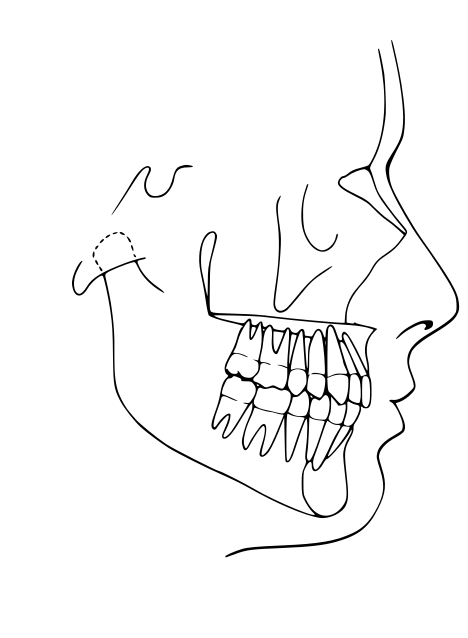
\includegraphics[width=\textwidth]{./images/face.pdf}
% \caption{Punti di repere cefalometrici}
%\end{figure}

%\begin{refsegment}
\normalsize
\printbibliography
%\end{refsegment}

\end{document}
